%% fig_mumford.tex   (generated by make_mumford.py; do not edit by hand)
%% The weight two cohomology of a Mumford fourfold over the triangle of the three factors, with the map mu, the Galois arcs and the K3 surface above.
\documentclass[tikz,border=8pt]{standalone}
\usepackage{amsmath,amssymb}
\usetikzlibrary{arrows.meta,calc}
%% palette.tex -- shared colour definitions for the figures
\definecolor{PInk}{RGB}{26,32,44}
\definecolor{PBlue}{RGB}{37,82,139}
\definecolor{PTeal}{RGB}{23,127,125}
\definecolor{POchre}{RGB}{193,138,44}
\definecolor{PClay}{RGB}{178,74,58}
\definecolor{PSlate}{RGB}{108,122,137}
\definecolor{PViolet}{RGB}{110,86,150}
\definecolor{WBlue}{RGB}{223,234,246}
\definecolor{WTeal}{RGB}{220,238,236}
\definecolor{WOchre}{RGB}{250,240,218}
\definecolor{WClay}{RGB}{247,229,224}
\definecolor{WSlate}{RGB}{238,241,244}
\definecolor{PMag}{RGB}{158,58,110}
\definecolor{PGrass}{RGB}{62,124,66}
\definecolor{PAmber}{RGB}{214,112,38}
\definecolor{PIndigo}{RGB}{58,64,140}
\definecolor{PRule}{RGB}{176,186,197}

%% shared macros so the standalone figures match the paper
\providecommand{\QQ}{\mathbb{Q}}
\providecommand{\ZZ}{\mathbb{Z}}
\providecommand{\RR}{\mathbb{R}}
\providecommand{\CC}{\mathbb{C}}
\providecommand{\PP}{\mathbb{P}}
\providecommand{\Kx}{K^{\times}}
\providecommand{\HW}{W}
\providecommand{\Nm}{\mathrm{N}}
\providecommand{\Hdg}{\mathrm{Hdg}}
\providecommand{\NS}{\mathrm{NS}}
\providecommand{\cA}{\mathcal{A}}
\providecommand{\cD}{\mathcal{D}}
\providecommand{\cF}{\mathcal{F}}
\providecommand{\cP}{\mathcal{P}}
\providecommand{\cO}{\mathcal{O}}
\providecommand{\cQ}{\mathcal{Q}}
\providecommand{\bbar}[1]{\overline{#1}}
\providecommand{\ch}{\operatorname{ch}}
\providecommand{\End}{\mathrm{End}}

\begin{document}
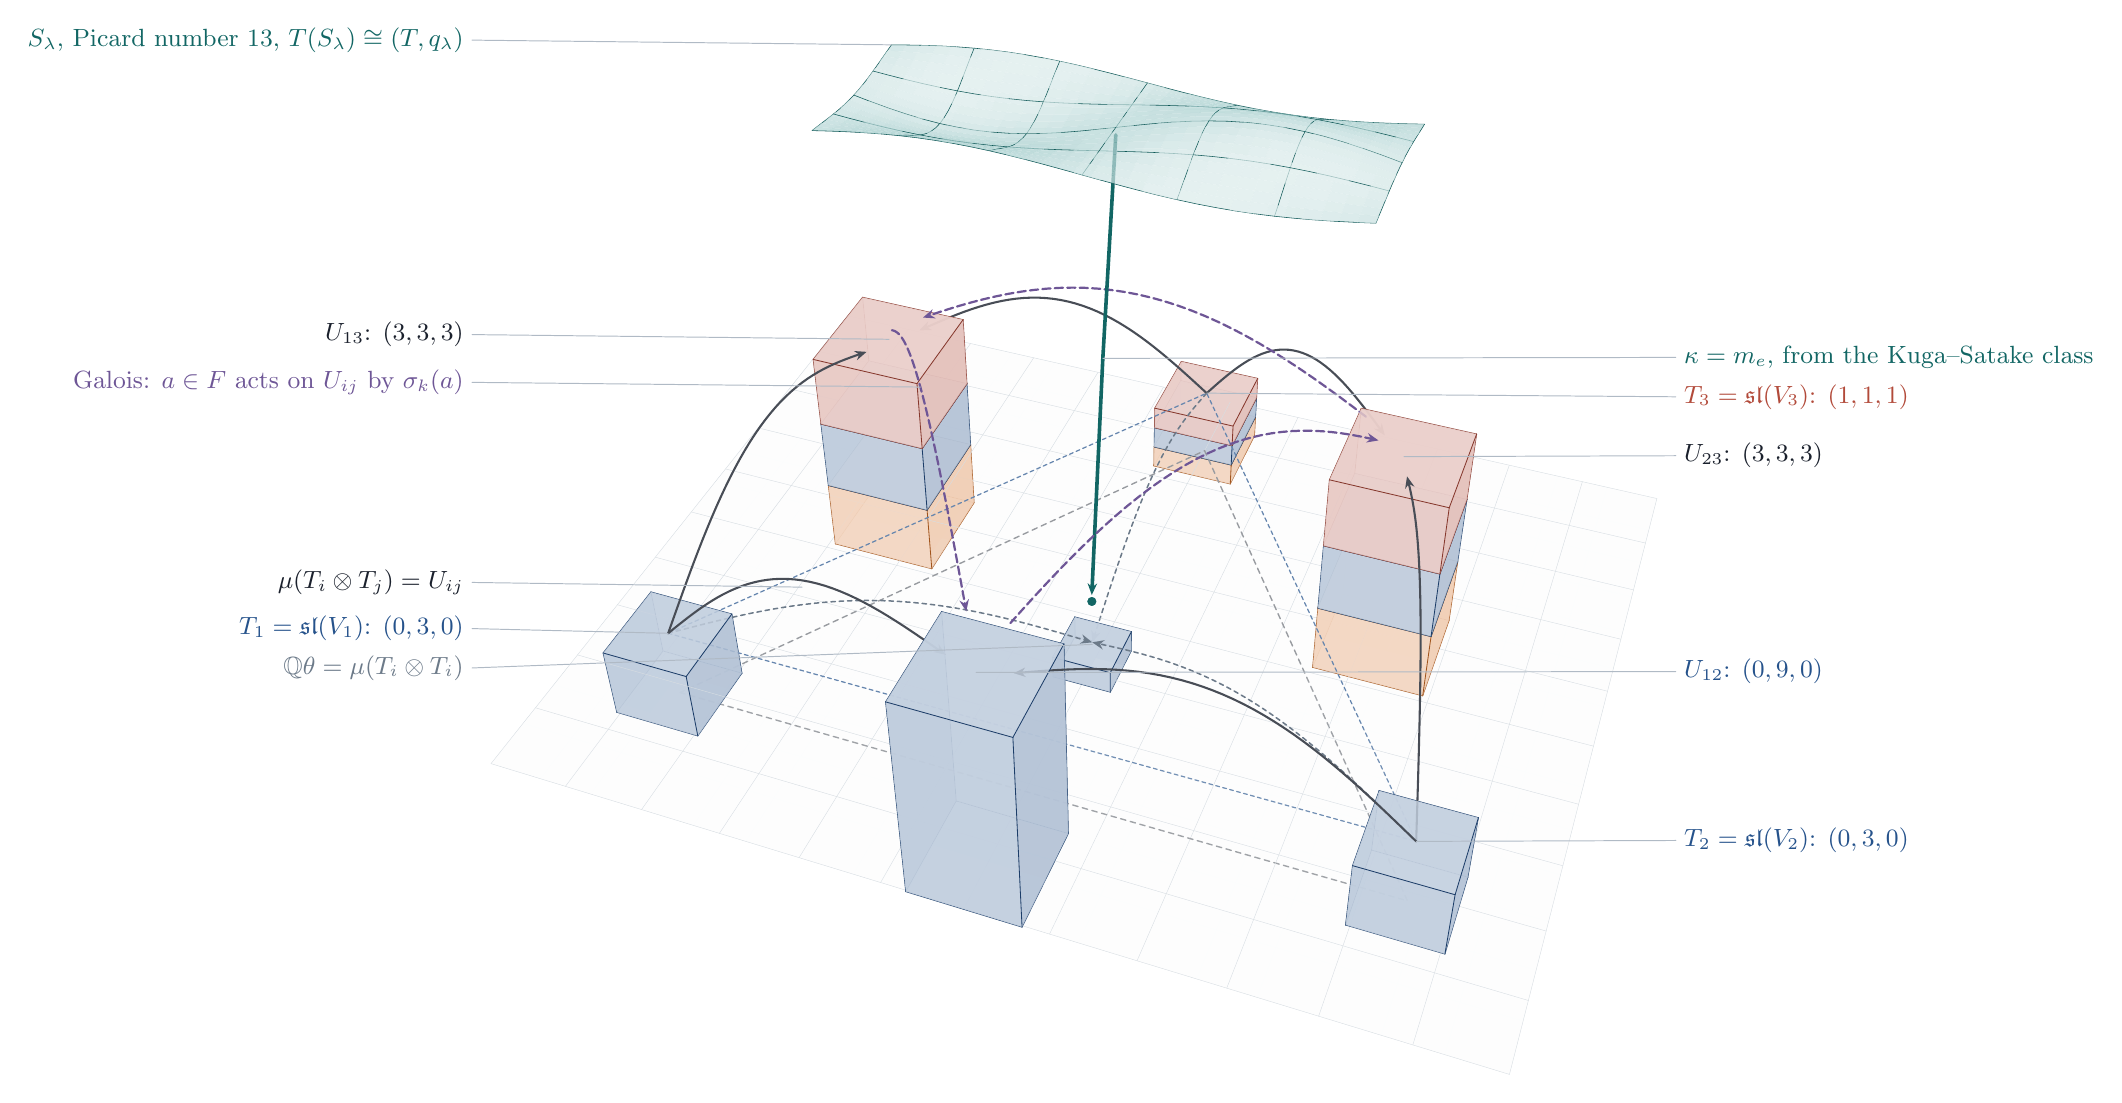
\begin{tikzpicture}[x=1cm,y=1cm,line join=round,line cap=round,
  font=\small,text=PInk]
  \path[draw=none,fill opacity=0.10,fill=PSlate!16!white] (-3.6640,1.7715) -- (-3.1422,1.6514) -- (-2.8928,1.9771) -- (-3.4078,2.0934) -- cycle;
  \path[draw=none,fill opacity=0.10,fill=PSlate!16!white] (-3.1422,1.6514) -- (-2.6142,1.5299) -- (-2.3717,1.8594) -- (-2.8928,1.9771) -- cycle;
  \path[draw=none,fill opacity=0.10,fill=PSlate!16!white] (-2.6142,1.5299) -- (-2.0800,1.4070) -- (-1.8446,1.7404) -- (-2.3717,1.8594) -- cycle;
  \path[draw=none,fill opacity=0.10,fill=PSlate!16!white] (-3.9285,1.4391) -- (-3.3998,1.3151) -- (-3.1422,1.6514) -- (-3.6640,1.7715) -- cycle;
  \path[draw=none,fill opacity=0.10,fill=PSlate!16!white] (-2.0800,1.4070) -- (-1.5394,1.2826) -- (-1.3113,1.6199) -- (-1.8446,1.7404) -- cycle;
  \path[draw=none,fill opacity=0.10,fill=PSlate!16!white] (-3.3998,1.3151) -- (-2.8647,1.1896) -- (-2.6142,1.5299) -- (-3.1422,1.6514) -- cycle;
  \path[draw=none,fill opacity=0.10,fill=PSlate!16!white] (-1.5394,1.2826) -- (-0.9922,1.1567) -- (-0.7717,1.4981) -- (-1.3113,1.6199) -- cycle;
  \path[draw=none,fill opacity=0.10,fill=PSlate!16!white] (-2.8647,1.1896) -- (-2.3231,1.0626) -- (-2.0800,1.4070) -- (-2.6142,1.5299) -- cycle;
  \path[draw=none,fill opacity=0.10,fill=PSlate!16!white] (-0.9922,1.1567) -- (-0.4385,1.0292) -- (-0.2257,1.3747) -- (-0.7717,1.4981) -- cycle;
  \path[draw=none,fill opacity=0.10,fill=PSlate!16!white] (-4.2018,1.0958) -- (-3.6659,0.9676) -- (-3.3998,1.3151) -- (-3.9285,1.4391) -- cycle;
  \path[draw=none,fill opacity=0.10,fill=PSlate!16!white] (-2.3231,1.0626) -- (-1.7750,0.9340) -- (-1.5394,1.2826) -- (-2.0800,1.4070) -- cycle;
  \path[draw=none,fill opacity=0.10,fill=PSlate!16!white] (-0.4385,1.0292) -- (0.1219,0.9002) -- (0.3268,1.2499) -- (-0.2257,1.3747) -- cycle;
  \path[draw=none,fill opacity=0.10,fill=PSlate!16!white] (-3.6659,0.9676) -- (-3.1235,0.8379) -- (-2.8647,1.1896) -- (-3.3998,1.3151) -- cycle;
  \path[draw=none,fill opacity=0.10,fill=PSlate!16!white] (-1.7750,0.9340) -- (-1.2201,0.8038) -- (-0.9922,1.1567) -- (-1.5394,1.2826) -- cycle;
  \path[draw=none,fill opacity=0.10,fill=PSlate!16!white] (0.1219,0.9002) -- (0.6893,0.7697) -- (0.8860,1.1236) -- (0.3268,1.2499) -- cycle;
  \draw[PRule!50,line width=0.15pt] (-3.4078,2.0934) -- (6.8719,-0.2284);
  \path[draw=none,fill opacity=0.10,fill=PSlate!16!white] (-3.1235,0.8379) -- (-2.5744,0.7065) -- (-2.3231,1.0626) -- (-2.8647,1.1896) -- cycle;
  \path[draw=none,fill opacity=0.10,fill=PSlate!16!white] (-1.2201,0.8038) -- (-0.6585,0.6721) -- (-0.4385,1.0292) -- (-0.9922,1.1567) -- cycle;
  \path[draw=none,fill opacity=0.10,fill=PSlate!16!white] (0.6893,0.7697) -- (1.2636,0.6375) -- (1.4520,0.9958) -- (0.8860,1.1236) -- cycle;
  \path[draw=none,fill opacity=0.10,fill=PSlate!16!white] (-4.4842,0.7409) -- (-3.9410,0.6084) -- (-3.6659,0.9676) -- (-4.2018,1.0958) -- cycle;
  \path[draw=none,fill opacity=0.10,fill=PSlate!16!white] (-2.5744,0.7065) -- (-2.0185,0.5736) -- (-1.7750,0.9340) -- (-2.3231,1.0626) -- cycle;
  \path[draw=none,fill opacity=0.10,fill=PSlate!16!white] (-0.6585,0.6721) -- (-0.0899,0.5387) -- (0.1219,0.9002) -- (-0.4385,1.0292) -- cycle;
  \path[draw=none,fill opacity=0.10,fill=PSlate!16!white] (1.2636,0.6375) -- (1.8450,0.5037) -- (2.0249,0.8664) -- (1.4520,0.9958) -- cycle;
  \path[draw=none,fill opacity=0.10,fill=PSlate!16!white] (-3.9410,0.6084) -- (-3.3911,0.4742) -- (-3.1235,0.8379) -- (-3.6659,0.9676) -- cycle;
  \draw[PAmber!75!black,line width=0.3pt] (0.8136,0.7858) -- (0.8199,1.0241);
  \path[draw=none,fill opacity=0.10,fill=PSlate!16!white] (-2.0185,0.5736) -- (-1.4558,0.4390) -- (-1.2201,0.8038) -- (-1.7750,0.9340) -- cycle;
  \draw[PAmber!75!black,line width=0.3pt] (0.8136,0.7858) -- (1.7605,0.5684);
  \path[draw=none,fill opacity=0.10,fill=PSlate!16!white] (-0.0899,0.5387) -- (0.4858,0.4037) -- (0.6893,0.7697) -- (0.1219,0.9002) -- cycle;
  \path[draw=none,fill opacity=0.10,fill=PSlate!16!white] (1.8450,0.5037) -- (2.4337,0.3682) -- (2.6048,0.7354) -- (2.0249,0.8664) -- cycle;
  \path[draw=none,fill opacity=0.80,fill=PAmber!28!white] (0.8136,0.7858) -- (1.7605,0.5684) -- (1.7741,0.8074) -- (0.8199,1.0241) -- cycle;
  \path[draw=none,fill opacity=0.10,fill=PSlate!16!white] (-3.3911,0.4742) -- (-2.8343,0.3384) -- (-2.5744,0.7065) -- (-3.1235,0.8379) -- cycle;
  \path[draw=none,fill opacity=0.10,fill=PSlate!16!white] (-1.4558,0.4390) -- (-0.8860,0.3027) -- (-0.6585,0.6721) -- (-1.2201,0.8038) -- cycle;
  \draw[PBlue!75!black,line width=0.3pt] (0.8199,1.0241) -- (0.8262,1.2661);
  \path[draw=none,fill opacity=0.10,fill=PSlate!16!white] (0.4858,0.4037) -- (1.0687,0.2670) -- (1.2636,0.6375) -- (0.6893,0.7697) -- cycle;
  \draw[PAmber!75!black,line width=0.3pt] (0.8199,1.0241) -- (1.7741,0.8074);
  \draw[PBlue!75!black,line width=0.3pt] (0.8199,1.0241) -- (1.7741,0.8074);
  \path[draw=none,fill opacity=0.10,fill=PSlate!16!white] (-4.7763,0.3739) -- (-4.2256,0.2368) -- (-3.9410,0.6084) -- (-4.4842,0.7409) -- cycle;
  \draw[PRule!50,line width=0.15pt] (-3.7688,1.6398) -- (6.7271,-0.7940);
  \draw[PAmber!75!black,line width=0.3pt] (0.4837,0.1865) -- (0.8136,0.7858);
  \path[draw=none,fill opacity=0.10,fill=PSlate!16!white] (2.4337,0.3682) -- (3.0297,0.2311) -- (3.1918,0.6028) -- (2.6048,0.7354) -- cycle;
  \draw[PAmber!75!black,line width=0.3pt] (1.7605,0.5684) -- (1.7741,0.8074);
  \path[draw=none,fill opacity=0.10,fill=PSlate!16!white] (-2.8343,0.3384) -- (-2.2705,0.2008) -- (-2.0185,0.5736) -- (-2.5744,0.7065) -- cycle;
  \path[draw=none,fill opacity=0.80,fill=PBlue!28!white] (0.8199,1.0241) -- (1.7741,0.8074) -- (1.7879,1.0503) -- (0.8262,1.2661) -- cycle;
  \path[draw=none,fill opacity=0.10,fill=PSlate!16!white] (-0.8860,0.3027) -- (-0.3090,0.1647) -- (-0.0899,0.5387) -- (-0.6585,0.6721) -- cycle;
  \path[draw=none,fill opacity=0.80,fill=PAmber!35!white] (0.4837,0.1865) -- (0.8136,0.7858) -- (0.8199,1.0241) -- (0.4875,0.4268) -- cycle;
  \path[draw=none,fill opacity=0.10,fill=PSlate!16!white] (1.0687,0.2670) -- (1.6589,0.1285) -- (1.8450,0.5037) -- (1.2636,0.6375) -- cycle;
  \path[draw=none,fill opacity=0.80,fill=PAmber!26!white] (0.4837,0.1865) -- (1.4538,-0.0433) -- (1.7605,0.5684) -- (0.8136,0.7858) -- cycle;
  \draw[PClay!75!black,line width=0.3pt] (0.8262,1.2661) -- (0.8326,1.5119);
  \path[draw=none,fill opacity=0.10,fill=PSlate!16!white] (-4.2256,0.2368) -- (-3.6679,0.0980) -- (-3.3911,0.4742) -- (-3.9410,0.6084) -- cycle;
  \path[draw=none,fill opacity=0.10,fill=PSlate!16!white] (3.0297,0.2311) -- (3.6333,0.0922) -- (3.7861,0.4686) -- (3.1918,0.6028) -- cycle;
  \draw[PBlue!75!black,line width=0.3pt] (0.8262,1.2661) -- (1.7879,1.0503);
  \draw[PClay!75!black,line width=0.3pt] (0.8262,1.2661) -- (1.7879,1.0503);
  \draw[PAmber!75!black,line width=0.3pt] (0.4875,0.4268) -- (0.8199,1.0241);
  \draw[PBlue!75!black,line width=0.3pt] (0.4875,0.4268) -- (0.8199,1.0241);
  \path[draw=none,fill opacity=0.10,fill=PSlate!16!white] (-2.2705,0.2008) -- (-1.6996,0.0615) -- (-1.4558,0.4390) -- (-2.0185,0.5736) -- cycle;
  \draw[PBlue!75!black,line width=0.3pt] (1.7741,0.8074) -- (1.7879,1.0503);
  \path[draw=none,fill opacity=0.10,fill=PSlate!16!white] (-0.3090,0.1647) -- (0.2753,0.0250) -- (0.4858,0.4037) -- (-0.0899,0.5387) -- cycle;
  \draw[PAmber!75!black,line width=0.3pt] (1.4538,-0.0433) -- (1.7605,0.5684);
  \path[draw=none,fill opacity=0.80,fill=PClay!28!white] (0.8262,1.2661) -- (1.7879,1.0503) -- (1.8020,1.2969) -- (0.8326,1.5119) -- cycle;
  \path[draw=none,fill opacity=0.10,fill=PSlate!16!white] (1.6589,0.1285) -- (2.2566,-0.0117) -- (2.4337,0.3682) -- (1.8450,0.5037) -- cycle;
  \path[draw=none,fill opacity=0.80,fill=PBlue!35!white] (0.4875,0.4268) -- (0.8199,1.0241) -- (0.8262,1.2661) -- (0.4914,0.6710) -- cycle;
  \path[draw=none,fill opacity=0.10,fill=PSlate!16!white] (-3.6679,0.0980) -- (-3.1032,-0.0426) -- (-2.8343,0.3384) -- (-3.3911,0.4742) -- cycle;
  \path[draw=none,fill opacity=0.10,fill=PSlate!16!white] (3.6333,0.0922) -- (4.2445,-0.0485) -- (4.3879,0.3327) -- (3.7861,0.4686) -- cycle;
  \path[draw=none,fill opacity=0.80,fill=PAmber!26!white] (0.4875,0.4268) -- (1.4654,0.1977) -- (1.7741,0.8074) -- (0.8199,1.0241) -- cycle;
  \path[draw=none,fill opacity=0.80,fill=PBlue!26!white] (0.4875,0.4268) -- (1.4654,0.1977) -- (1.7741,0.8074) -- (0.8199,1.0241) -- cycle;
  \path[draw=none,fill opacity=0.10,fill=PSlate!16!white] (-1.6996,0.0615) -- (-1.1214,-0.0795) -- (-0.8860,0.3027) -- (-1.4558,0.4390) -- cycle;
  \path[draw=none,fill opacity=0.80,fill=PAmber!35!white] (1.4538,-0.0433) -- (1.7605,0.5684) -- (1.7741,0.8074) -- (1.4654,0.1977) -- cycle;
  \draw[PClay!75!black,line width=0.3pt] (0.8326,1.5119) -- (1.8020,1.2969);
  \draw[PBlue!75!black,line width=0.3pt] (0.4914,0.6710) -- (0.8262,1.2661);
  \draw[PClay!75!black,line width=0.3pt] (0.4914,0.6710) -- (0.8262,1.2661);
  \path[draw=none,fill opacity=0.10,fill=PSlate!16!white] (0.2753,0.0250) -- (0.8670,-0.1166) -- (1.0687,0.2670) -- (0.4858,0.4037) -- cycle;
  \draw[PClay!75!black,line width=0.3pt] (1.7879,1.0503) -- (1.8020,1.2969);
  \path[draw=none,fill opacity=0.10,fill=PSlate!16!white] (-5.0785,-0.0058) -- (-4.5201,-0.1478) -- (-4.2256,0.2368) -- (-4.7763,0.3739) -- cycle;
  \path[draw=none,fill opacity=0.10,fill=PSlate!16!white] (2.2566,-0.0117) -- (2.8620,-0.1537) -- (3.0297,0.2311) -- (2.4337,0.3682) -- cycle;
  \draw[PAmber!75!black,line width=0.3pt] (0.4837,0.1865) -- (0.4875,0.4268);
  \draw[PAmber!75!black,line width=0.3pt] (1.4654,0.1977) -- (1.7741,0.8074);
  \draw[PBlue!75!black,line width=0.3pt] (1.4654,0.1977) -- (1.7741,0.8074);
  \path[draw=none,fill opacity=0.10,fill=PSlate!16!white] (-3.1032,-0.0426) -- (-2.5313,-0.1850) -- (-2.2705,0.2008) -- (-2.8343,0.3384) -- cycle;
  \path[draw=none,fill opacity=0.10,fill=PSlate!16!white] (4.2445,-0.0485) -- (4.8636,-0.1910) -- (4.9972,0.1951) -- (4.3879,0.3327) -- cycle;
  \draw[PAmber!75!black,line width=0.3pt] (0.4837,0.1865) -- (1.4538,-0.0433);
  \path[draw=none,fill opacity=0.80,fill=PClay!35!white] (0.4914,0.6710) -- (0.8262,1.2661) -- (0.8326,1.5119) -- (0.4953,0.9190) -- cycle;
  \path[draw=none,fill opacity=0.10,fill=PSlate!16!white] (-1.1214,-0.0795) -- (-0.5358,-0.2224) -- (-0.3090,0.1647) -- (-0.8860,0.3027) -- cycle;
  \path[draw=none,fill opacity=0.80,fill=PBlue!26!white] (0.4914,0.6710) -- (1.4771,0.4426) -- (1.7879,1.0503) -- (0.8262,1.2661) -- cycle;
  \path[draw=none,fill opacity=0.80,fill=PClay!26!white] (0.4914,0.6710) -- (1.4771,0.4426) -- (1.7879,1.0503) -- (0.8262,1.2661) -- cycle;
  \path[draw=none,fill opacity=0.80,fill=PBlue!35!white] (1.4654,0.1977) -- (1.7741,0.8074) -- (1.7879,1.0503) -- (1.4771,0.4426) -- cycle;
  \path[draw=none,fill opacity=0.10,fill=PSlate!16!white] (0.8670,-0.1166) -- (1.4663,-0.2599) -- (1.6589,0.1285) -- (1.0687,0.2670) -- cycle;
  \path[draw=none,fill opacity=0.80,fill=PAmber!28!white] (0.4837,0.1865) -- (1.4538,-0.0433) -- (1.4654,0.1977) -- (0.4875,0.4268) -- cycle;
  \path[draw=none,fill opacity=0.10,fill=PSlate!16!white] (-4.5201,-0.1478) -- (-3.9545,-0.2915) -- (-3.6679,0.0980) -- (-4.2256,0.2368) -- cycle;
  \draw[PClay!75!black,line width=0.3pt] (0.4953,0.9190) -- (0.8326,1.5119);
  \path[draw=none,fill opacity=0.10,fill=PSlate!16!white] (2.8620,-0.1537) -- (3.4751,-0.2975) -- (3.6333,0.0922) -- (3.0297,0.2311) -- cycle;
  \draw[PRule!50,line width=0.15pt] (-4.1464,1.1654) -- (6.5748,-1.3889);
  \path[draw=none,fill opacity=0.10,fill=PSlate!16!white] (-2.5313,-0.1850) -- (-1.9520,-0.3292) -- (-1.6996,0.0615) -- (-2.2705,0.2008) -- cycle;
  \path[draw=none,fill opacity=0.10,fill=PSlate!16!white] (4.8636,-0.1910) -- (5.4906,-0.3353) -- (5.6142,0.0557) -- (4.9972,0.1951) -- cycle;
  \draw[PBlue!75!black,line width=0.3pt] (0.4875,0.4268) -- (0.4914,0.6710);
  \draw[PBlue!75!black,line width=0.3pt] (1.4771,0.4426) -- (1.7879,1.0503);
  \draw[PClay!75!black,line width=0.3pt] (1.4771,0.4426) -- (1.7879,1.0503);
  \path[draw=none,fill opacity=0.10,fill=PSlate!16!white] (-0.5358,-0.2224) -- (0.0573,-0.3671) -- (0.2753,0.0250) -- (-0.3090,0.1647) -- cycle;
  \draw[PAmber!75!black,line width=0.3pt] (0.4875,0.4268) -- (1.4654,0.1977);
  \draw[PBlue!75!black,line width=0.3pt] (0.4875,0.4268) -- (1.4654,0.1977);
  \draw[PAmber!75!black,line width=0.3pt] (1.4538,-0.0433) -- (1.4654,0.1977);
  \draw[PAmber!75!black,line width=0.3pt] (-2.9874,0.0126) -- (-1.7999,-0.2819);
  \path[draw=none,fill opacity=0.10,fill=PSlate!16!white] (1.4663,-0.2599) -- (2.0733,-0.4051) -- (2.2566,-0.0117) -- (1.6589,0.1285) -- cycle;
  \path[draw=none,fill opacity=0.80,fill=PClay!26!white] (0.4953,0.9190) -- (1.4891,0.6915) -- (1.8020,1.2969) -- (0.8326,1.5119) -- cycle;
  \path[draw=none,fill opacity=0.10,fill=PSlate!16!white] (-3.9545,-0.2915) -- (-3.3817,-0.4371) -- (-3.1032,-0.0426) -- (-3.6679,0.0980) -- cycle;
  \path[draw=none,fill opacity=0.80,fill=PClay!35!white] (1.4771,0.4426) -- (1.7879,1.0503) -- (1.8020,1.2969) -- (1.4891,0.6915) -- cycle;
  \path[draw=none,fill opacity=0.10,fill=PSlate!16!white] (3.4751,-0.2975) -- (4.0961,-0.4432) -- (4.2445,-0.0485) -- (3.6333,0.0922) -- cycle;
  \path[draw=none,fill opacity=0.80,fill=PBlue!28!white] (0.4875,0.4268) -- (1.4654,0.1977) -- (1.4771,0.4426) -- (0.4914,0.6710) -- cycle;
  \path[draw=none,fill opacity=0.10,fill=PSlate!16!white] (-1.9520,-0.3292) -- (-1.3652,-0.4753) -- (-1.1214,-0.0795) -- (-1.6996,0.0615) -- cycle;
  \path[draw=none,fill opacity=0.10,fill=PSlate!16!white] (5.4906,-0.3353) -- (6.1258,-0.4814) -- (6.2390,-0.0854) -- (5.6142,0.0557) -- cycle;
  \path[draw=none,fill opacity=0.10,fill=PSlate!16!white] (0.0573,-0.3671) -- (0.6581,-0.5137) -- (0.8670,-0.1166) -- (0.2753,0.0250) -- cycle;
  \draw[PClay!75!black,line width=0.3pt] (0.4914,0.6710) -- (0.4953,0.9190);
  \draw[PAmber!75!black,line width=0.3pt] (-2.9874,0.0126) -- (-3.0597,0.7468);
  \draw[PClay!75!black,line width=0.3pt] (1.4891,0.6915) -- (1.8020,1.2969);
  \path[draw=none,fill opacity=0.10,fill=PSlate!16!white] (-5.3914,-0.3990) -- (-4.8251,-0.5460) -- (-4.5201,-0.1478) -- (-5.0785,-0.0058) -- cycle;
  \path[draw=none,fill opacity=0.10,fill=PSlate!16!white] (2.0733,-0.4051) -- (2.6883,-0.5522) -- (2.8620,-0.1537) -- (2.2566,-0.0117) -- cycle;
  \draw[PBlue!75!black,line width=0.3pt] (0.4914,0.6710) -- (1.4771,0.4426);
  \draw[PClay!75!black,line width=0.3pt] (0.4914,0.6710) -- (1.4771,0.4426);
  \path[draw=none,fill opacity=0.10,fill=PSlate!16!white] (-3.3817,-0.4371) -- (-2.8013,-0.5846) -- (-2.5313,-0.1850) -- (-3.1032,-0.0426) -- cycle;
  \draw[PBlue!75!black,line width=0.3pt] (1.4654,0.1977) -- (1.4771,0.4426);
  \path[draw=none,fill opacity=0.10,fill=PSlate!16!white] (4.0961,-0.4432) -- (4.7253,-0.5908) -- (4.8636,-0.1910) -- (4.2445,-0.0485) -- cycle;
  \path[draw=none,fill opacity=0.10,fill=PSlate!16!white] (-1.3652,-0.4753) -- (-0.7707,-0.6233) -- (-0.5358,-0.2224) -- (-1.1214,-0.0795) -- cycle;
  \path[draw=none,fill opacity=0.10,fill=PSlate!16!white] (6.1258,-0.4814) -- (6.7692,-0.6295) -- (6.8719,-0.2284) -- (6.2390,-0.0854) -- cycle;
  \path[draw=none,fill opacity=0.80,fill=PClay!28!white] (0.4914,0.6710) -- (1.4771,0.4426) -- (1.4891,0.6915) -- (0.4953,0.9190) -- cycle;
  \path[draw=none,fill opacity=0.10,fill=PSlate!16!white] (0.6581,-0.5137) -- (1.2668,-0.6622) -- (1.4663,-0.2599) -- (0.8670,-0.1166) -- cycle;
  \draw[PAmber!75!black,line width=0.3pt] (-3.5607,-0.8036) -- (-2.9874,0.0126);
  \draw[PRule!50,line width=0.15pt] (-7.9351,-3.5953) -- (-3.4078,2.0934);
  \path[draw=none,fill opacity=0.80,fill=PAmber!28!white] (-2.9874,0.0126) -- (-1.7999,-0.2819) -- (-1.8440,0.4551) -- (-3.0597,0.7468) -- cycle;
  \path[draw=none,fill opacity=0.10,fill=PSlate!16!white] (-4.8251,-0.5460) -- (-4.2514,-0.6949) -- (-3.9545,-0.2915) -- (-4.5201,-0.1478) -- cycle;
  \path[draw=none,fill opacity=0.10,fill=PSlate!16!white] (2.6883,-0.5522) -- (3.3112,-0.7012) -- (3.4751,-0.2975) -- (2.8620,-0.1537) -- cycle;
  \path[draw=none,fill opacity=0.10,fill=PSlate!16!white] (-2.8013,-0.5846) -- (-2.2134,-0.7340) -- (-1.9520,-0.3292) -- (-2.5313,-0.1850) -- cycle;
  \path[draw=none,fill opacity=0.10,fill=PSlate!16!white] (4.7253,-0.5908) -- (5.3626,-0.7403) -- (5.4906,-0.3353) -- (4.8636,-0.1910) -- cycle;
  \draw[PClay!75!black,line width=0.3pt] (0.4953,0.9190) -- (1.4891,0.6915);
  \draw[PClay!75!black,line width=0.3pt] (1.4771,0.4426) -- (1.4891,0.6915);
  \path[draw=none,fill opacity=0.10,fill=PSlate!16!white] (-0.7707,-0.6233) -- (-0.1685,-0.7733) -- (0.0573,-0.3671) -- (-0.5358,-0.2224) -- cycle;
  \path[draw=none,fill opacity=0.10,fill=PSlate!16!white] (1.2668,-0.6622) -- (1.8834,-0.8126) -- (2.0733,-0.4051) -- (1.4663,-0.2599) -- cycle;
  \path[draw=none,fill opacity=0.80,fill=PAmber!26!white] (-3.5607,-0.8036) -- (-2.3369,-1.1203) -- (-1.7999,-0.2819) -- (-2.9874,0.0126) -- cycle;
  \draw[PAmber!75!black,line width=0.3pt] (-1.7999,-0.2819) -- (-1.8440,0.4551);
  \path[draw=none,fill opacity=0.10,fill=PSlate!16!white] (-4.2514,-0.6949) -- (-3.6701,-0.8458) -- (-3.3817,-0.4371) -- (-3.9545,-0.2915) -- cycle;
  \path[draw=none,fill opacity=0.10,fill=PSlate!16!white] (3.3112,-0.7012) -- (3.9424,-0.8521) -- (4.0961,-0.4432) -- (3.4751,-0.2975) -- cycle;
  \draw[PRule!50,line width=0.15pt] (-4.5418,0.6685) -- (6.4144,-2.0153);
  \path[draw=none,fill opacity=0.10,fill=PSlate!16!white] (-2.2134,-0.7340) -- (-1.6177,-0.8854) -- (-1.3652,-0.4753) -- (-1.9520,-0.3292) -- cycle;
  \path[draw=none,fill opacity=0.10,fill=PSlate!16!white] (5.3626,-0.7403) -- (6.0084,-0.8918) -- (6.1258,-0.4814) -- (5.4906,-0.3353) -- cycle;
  \draw[PRule!50,line width=0.15pt] (-6.9896,-3.8838) -- (-2.6330,1.9184);
  \path[draw=none,fill opacity=0.10,fill=PSlate!16!white] (-0.1685,-0.7733) -- (0.4417,-0.9252) -- (0.6581,-0.5137) -- (0.0573,-0.3671) -- cycle;
  \path[draw=none,fill opacity=0.80,fill=PAmber!35!white] (-3.5607,-0.8036) -- (-2.9874,0.0126) -- (-3.0597,0.7468) -- (-3.6501,-0.0622) -- cycle;
  \path[draw=none,fill opacity=0.10,fill=PSlate!16!white] (-5.7155,-0.8063) -- (-5.1411,-0.9587) -- (-4.8251,-0.5460) -- (-5.3914,-0.3990) -- cycle;
  \draw[PAmber!75!black,line width=0.3pt] (-3.0597,0.7468) -- (-1.8440,0.4551);
  \draw[PBlue!75!black,line width=0.3pt] (-3.0597,0.7468) -- (-1.8440,0.4551);
  \path[draw=none,fill opacity=0.10,fill=PSlate!16!white] (1.8834,-0.8126) -- (2.5082,-0.9651) -- (2.6883,-0.5522) -- (2.0733,-0.4051) -- cycle;
  \draw[PAmber!75!black,line width=0.3pt] (-2.3369,-1.1203) -- (-1.7999,-0.2819);
  \path[draw=none,fill opacity=0.10,fill=PSlate!16!white] (-3.6701,-0.8458) -- (-3.0812,-0.9987) -- (-2.8013,-0.5846) -- (-3.3817,-0.4371) -- cycle;
  \path[draw=none,fill opacity=0.10,fill=PSlate!16!white] (3.9424,-0.8521) -- (4.5819,-1.0051) -- (4.7253,-0.5908) -- (4.0961,-0.4432) -- cycle;
  \path[draw=none,fill opacity=0.10,fill=PSlate!16!white] (-1.6177,-0.8854) -- (-1.0142,-1.0388) -- (-0.7707,-0.6233) -- (-1.3652,-0.4753) -- cycle;
  \path[draw=none,fill opacity=0.10,fill=PSlate!16!white] (6.0084,-0.8918) -- (6.6628,-1.0452) -- (6.7692,-0.6295) -- (6.1258,-0.4814) -- cycle;
  \path[draw=none,fill opacity=0.10,fill=PSlate!16!white] (0.4417,-0.9252) -- (1.0600,-1.0791) -- (1.2668,-0.6622) -- (0.6581,-0.5137) -- cycle;
  \draw[PBlue!75!black,line width=0.3pt] (-3.0597,0.7468) -- (-3.1356,1.5175);
  \path[draw=none,fill opacity=0.10,fill=PSlate!16!white] (-5.1411,-0.9587) -- (-4.5591,-1.1131) -- (-4.2514,-0.6949) -- (-4.8251,-0.5460) -- cycle;
  \path[draw=none,fill opacity=0.10,fill=PSlate!16!white] (2.5082,-0.9651) -- (3.1414,-1.1195) -- (3.3112,-0.7012) -- (2.6883,-0.5522) -- cycle;
  \draw[PRule!50,line width=0.15pt] (-6.0228,-4.1788) -- (-1.8446,1.7404);
  \path[draw=none,fill opacity=0.10,fill=PSlate!16!white] (-3.0812,-0.9987) -- (-2.4844,-1.1536) -- (-2.2134,-0.7340) -- (-2.8013,-0.5846) -- cycle;
  \path[draw=none,fill opacity=0.10,fill=PSlate!16!white] (4.5819,-1.0051) -- (5.2300,-1.1601) -- (5.3626,-0.7403) -- (4.7253,-0.5908) -- cycle;
  \path[draw=none,fill opacity=0.10,fill=PSlate!16!white] (-1.0142,-1.0388) -- (-0.4025,-1.1943) -- (-0.1685,-0.7733) -- (-0.7707,-0.6233) -- cycle;
  \path[draw=none,fill opacity=0.10,fill=PSlate!16!white] (1.0600,-1.0791) -- (1.6866,-1.2351) -- (1.8834,-0.8126) -- (1.2668,-0.6622) -- cycle;
  \draw[PAmber!75!black,line width=0.3pt] (-3.6501,-0.0622) -- (-3.0597,0.7468);
  \draw[PBlue!75!black,line width=0.3pt] (-3.6501,-0.0622) -- (-3.0597,0.7468);
  \draw[PAmber!75!black,line width=0.3pt] (-3.5607,-0.8036) -- (-2.3369,-1.1203);
  \path[draw=none,fill opacity=0.80,fill=PBlue!28!white] (-3.0597,0.7468) -- (-1.8440,0.4551) -- (-1.8904,1.2291) -- (-3.1356,1.5175) -- cycle;
  \path[draw=none,fill opacity=0.80,fill=PAmber!35!white] (-2.3369,-1.1203) -- (-1.7999,-0.2819) -- (-1.8440,0.4551) -- (-2.3964,-0.3765) -- cycle;
  \path[draw=none,fill opacity=0.10,fill=PSlate!16!white] (-4.5591,-1.1131) -- (-3.9692,-1.2695) -- (-3.6701,-0.8458) -- (-4.2514,-0.6949) -- cycle;
  \path[draw=none,fill opacity=0.10,fill=PSlate!16!white] (3.1414,-1.1195) -- (3.7830,-1.2761) -- (3.9424,-0.8521) -- (3.3112,-0.7012) -- cycle;
  \path[draw=none,fill opacity=0.10,fill=PSlate!16!white] (-2.4844,-1.1536) -- (-1.8796,-1.3106) -- (-1.6177,-0.8854) -- (-2.2134,-0.7340) -- cycle;
  \path[draw=none,fill opacity=0.10,fill=PSlate!16!white] (5.2300,-1.1601) -- (5.8867,-1.3172) -- (6.0084,-0.8918) -- (5.3626,-0.7403) -- cycle;
  \path[draw=none,fill opacity=0.10,fill=PSlate!16!white] (-0.4025,-1.1943) -- (0.2173,-1.3518) -- (0.4417,-0.9252) -- (-0.1685,-0.7733) -- cycle;
  \draw[PRule!50,line width=0.15pt] (-5.0339,-4.4806) -- (-1.0423,1.5592);
  \draw[PAmber!75!black,line width=0.3pt] (-3.5607,-0.8036) -- (-3.6501,-0.0622);
  \path[draw=none,fill opacity=0.10,fill=PSlate!16!white] (-6.0516,-1.2286) -- (-5.4688,-1.3866) -- (-5.1411,-0.9587) -- (-5.7155,-0.8063) -- cycle;
  \path[draw=none,fill opacity=0.10,fill=PSlate!16!white] (1.6866,-1.2351) -- (2.3216,-1.3932) -- (2.5082,-0.9651) -- (1.8834,-0.8126) -- cycle;
  \path[draw=none,fill opacity=0.80,fill=PAmber!26!white] (-3.6501,-0.0622) -- (-2.3964,-0.3765) -- (-1.8440,0.4551) -- (-3.0597,0.7468) -- cycle;
  \path[draw=none,fill opacity=0.80,fill=PBlue!26!white] (-3.6501,-0.0622) -- (-2.3964,-0.3765) -- (-1.8440,0.4551) -- (-3.0597,0.7468) -- cycle;
  \draw[PBlue!75!black,line width=0.3pt] (-1.8440,0.4551) -- (-1.8904,1.2291);
  \path[draw=none,fill opacity=0.10,fill=PSlate!16!white] (-3.9692,-1.2695) -- (-3.3714,-1.4281) -- (-3.0812,-0.9987) -- (-3.6701,-0.8458) -- cycle;
  \path[draw=none,fill opacity=0.10,fill=PSlate!16!white] (3.7830,-1.2761) -- (4.4333,-1.4347) -- (4.5819,-1.0051) -- (3.9424,-0.8521) -- cycle;
  \path[draw=none,fill opacity=0.10,fill=PSlate!16!white] (-1.8796,-1.3106) -- (-1.2666,-1.4697) -- (-1.0142,-1.0388) -- (-1.6177,-0.8854) -- cycle;
  \draw[PRule!50,line width=0.15pt] (-4.9563,0.1476) -- (6.2453,-2.6758);
  \path[draw=none,fill opacity=0.10,fill=PSlate!16!white] (5.8867,-1.3172) -- (6.5524,-1.4764) -- (6.6628,-1.0452) -- (6.0084,-0.8918) -- cycle;
  \path[draw=none,fill opacity=0.10,fill=PSlate!16!white] (0.2173,-1.3518) -- (0.8456,-1.5115) -- (1.0600,-1.0791) -- (0.4417,-0.9252) -- cycle;
  \path[draw=none,fill opacity=0.80,fill=PBlue!35!white] (-3.6501,-0.0622) -- (-3.0597,0.7468) -- (-3.1356,1.5175) -- (-3.7441,0.7174) -- cycle;
  \path[draw=none,fill opacity=0.10,fill=PSlate!16!white] (-5.4688,-1.3866) -- (-4.8782,-1.5467) -- (-4.5591,-1.1131) -- (-5.1411,-0.9587) -- cycle;
  \path[draw=none,fill opacity=0.80,fill=PAmber!28!white] (-3.5607,-0.8036) -- (-2.3369,-1.1203) -- (-2.3964,-0.3765) -- (-3.6501,-0.0622) -- cycle;
  \draw[PBlue!75!black,line width=0.3pt] (-3.1356,1.5175) -- (-1.8904,1.2291);
  \draw[PClay!75!black,line width=0.3pt] (-3.1356,1.5175) -- (-1.8904,1.2291);
  \path[draw=none,fill opacity=0.10,fill=PSlate!16!white] (2.3216,-1.3932) -- (2.9652,-1.5534) -- (3.1414,-1.1195) -- (2.5082,-0.9651) -- cycle;
  \draw[PAmber!75!black,line width=0.3pt] (-2.3964,-0.3765) -- (-1.8440,0.4551);
  \draw[PBlue!75!black,line width=0.3pt] (-2.3964,-0.3765) -- (-1.8440,0.4551);
  \path[draw=none,fill opacity=0.10,fill=PSlate!16!white] (-3.3714,-1.4281) -- (-2.7655,-1.5888) -- (-2.4844,-1.1536) -- (-3.0812,-0.9987) -- cycle;
  \path[draw=none,fill opacity=0.10,fill=PSlate!16!white] (4.4333,-1.4347) -- (5.0924,-1.5955) -- (5.2300,-1.1601) -- (4.5819,-1.0051) -- cycle;
  \draw[PRule!50,line width=0.15pt] (-4.0221,-4.7893) -- (-0.2257,1.3747);
  \path[draw=none,fill opacity=0.10,fill=PSlate!16!white] (-1.2666,-1.4697) -- (-0.6453,-1.6310) -- (-0.4025,-1.1943) -- (-1.0142,-1.0388) -- cycle;
  \path[draw=none,fill opacity=0.10,fill=PSlate!16!white] (0.8456,-1.5115) -- (1.4824,-1.6734) -- (1.6866,-1.2351) -- (1.0600,-1.0791) -- cycle;
  \draw[PClay!75!black,line width=0.3pt] (-3.1356,1.5175) -- (-3.2153,2.3273);
  \path[draw=none,fill opacity=0.10,fill=PSlate!16!white] (-4.8782,-1.5467) -- (-4.2795,-1.7091) -- (-3.9692,-1.2695) -- (-4.5591,-1.1131) -- cycle;
  \path[draw=none,fill opacity=0.10,fill=PSlate!16!white] (2.9652,-1.5534) -- (3.6176,-1.7159) -- (3.7830,-1.2761) -- (3.1414,-1.1195) -- cycle;
  \draw[PAmber!75!black,line width=0.3pt] (-2.3369,-1.1203) -- (-2.3964,-0.3765);
  \path[draw=none,fill opacity=0.10,fill=PSlate!16!white] (-2.7655,-1.5888) -- (-2.1513,-1.7517) -- (-1.8796,-1.3106) -- (-2.4844,-1.1536) -- cycle;
  \path[draw=none,fill opacity=0.10,fill=PSlate!16!white] (5.0924,-1.5955) -- (5.7605,-1.7585) -- (5.8867,-1.3172) -- (5.2300,-1.1601) -- cycle;
  \path[draw=none,fill opacity=0.10,fill=PSlate!16!white] (-0.6453,-1.6310) -- (-0.0155,-1.7945) -- (0.2173,-1.3518) -- (-0.4025,-1.1943) -- cycle;
  \draw[PInk!80,line width=0.75pt,-{Stealth[length=4.2pt,width=3.4pt]}] (1.1545,1.1097) -- (1.0729,1.1848) -- (0.9906,1.2602) -- (0.9076,1.3355) -- (0.8240,1.4103) -- (0.7396,1.4843) -- (0.6546,1.5571) -- (0.5688,1.6283) -- (0.4824,1.6977) -- (0.3953,1.7648) -- (0.3075,1.8293) -- (0.2190,1.8910) -- (0.1299,1.9494) -- (0.0402,2.0044) -- (-0.0501,2.0556) -- (-0.1410,2.1028) -- (-0.2324,2.1458) -- (-0.3243,2.1844) -- (-0.4166,2.2185) -- (-0.5094,2.2478) -- (-0.6025,2.2724) -- (-0.6960,2.2922) -- (-0.7897,2.3071) -- (-0.8838,2.3171) -- (-0.9780,2.3224) -- (-1.0725,2.3228) -- (-1.1670,2.3187) -- (-1.2617,2.3101) -- (-1.3565,2.2972) -- (-1.4513,2.2802) -- (-1.5462,2.2594) -- (-1.6411,2.2349) -- (-1.7359,2.2072) -- (-1.8308,2.1765) -- (-1.9256,2.1431) -- (-2.0204,2.1074) -- (-2.1152,2.0697) -- (-2.2100,2.0305) -- (-2.3048,1.9900) -- (-2.3996,1.9487) -- (-2.4945,1.9070);
  \draw[PSlate,line width=0.55pt,dash pattern=on 1.6pt off 1.4pt,-{Stealth[length=4.2pt,width=3.4pt]}] (1.1545,1.1097) -- (1.1229,1.0742) -- (1.0911,1.0382) -- (1.0591,1.0015) -- (1.0268,0.9639) -- (0.9942,0.9252) -- (0.9614,0.8850) -- (0.9283,0.8433) -- (0.8949,0.7998) -- (0.8612,0.7542) -- (0.8273,0.7065) -- (0.7931,0.6564) -- (0.7585,0.6037) -- (0.7237,0.5484) -- (0.6887,0.4902) -- (0.6533,0.4290) -- (0.6177,0.3648) -- (0.5818,0.2974) -- (0.5456,0.2267) -- (0.5092,0.1528) -- (0.4726,0.0755) -- (0.4357,-0.0051) -- (0.3985,-0.0890) -- (0.3612,-0.1762) -- (0.3236,-0.2667) -- (0.2859,-0.3604) -- (0.2480,-0.4572) -- (0.2098,-0.5570) -- (0.1715,-0.6596) -- (0.1331,-0.7650) -- (0.0945,-0.8731) -- (0.0557,-0.9835) -- (0.0169,-1.0963) -- (-0.0222,-1.2110) -- (-0.0613,-1.3277) -- (-0.1006,-1.4461) -- (-0.1399,-1.5658) -- (-0.1794,-1.6869) -- (-0.2190,-1.8089) -- (-0.2587,-1.9318) -- (-0.2986,-2.0552);
  \path[draw=none,fill opacity=0.10,fill=PSlate!16!white] (-6.4001,-1.6666) -- (-5.8088,-1.8306) -- (-5.4688,-1.3866) -- (-6.0516,-1.2286) -- cycle;
  \draw[PBlue!75!black,line width=0.3pt] (-3.7441,0.7174) -- (-3.1356,1.5175);
  \draw[PClay!75!black,line width=0.3pt] (-3.7441,0.7174) -- (-3.1356,1.5175);
  \path[draw=none,fill opacity=0.10,fill=PSlate!16!white] (1.4824,-1.6734) -- (2.1279,-1.8374) -- (2.3216,-1.3932) -- (1.6866,-1.2351) -- cycle;
  \draw[PAmber!75!black,line width=0.3pt] (-3.6501,-0.0622) -- (-2.3964,-0.3765);
  \draw[PBlue!75!black,line width=0.3pt] (-3.6501,-0.0622) -- (-2.3964,-0.3765);
  \path[draw=none,fill opacity=0.80,fill=PClay!28!white] (-3.1356,1.5175) -- (-1.8904,1.2291) -- (-1.9392,2.0431) -- (-3.2153,2.3273) -- cycle;
  \draw[PRule!50,line width=0.15pt] (-2.9867,-5.1052) -- (0.6056,1.1870);
  \path[draw=none,fill opacity=0.80,fill=PBlue!35!white] (-2.3964,-0.3765) -- (-1.8440,0.4551) -- (-1.8904,1.2291) -- (-2.4590,0.4061) -- cycle;
  \path[draw=none,fill opacity=0.10,fill=PSlate!16!white] (-4.2795,-1.7091) -- (-3.6726,-1.8736) -- (-3.3714,-1.4281) -- (-3.9692,-1.2695) -- cycle;
  \path[draw=none,fill opacity=0.10,fill=PSlate!16!white] (3.6176,-1.7159) -- (4.2790,-1.8805) -- (4.4333,-1.4347) -- (3.7830,-1.2761) -- cycle;
  \draw[PAmber!75!black,line width=0.3pt] (2.8822,-1.4432) -- (4.2316,-1.7779);
  \path[draw=none,fill opacity=0.10,fill=PSlate!16!white] (-2.1513,-1.7517) -- (-1.5286,-1.9169) -- (-1.2666,-1.4697) -- (-1.8796,-1.3106) -- cycle;
  \path[draw=none,fill opacity=0.10,fill=PSlate!16!white] (5.7605,-1.7585) -- (6.4378,-1.9238) -- (6.5524,-1.4764) -- (5.8867,-1.3172) -- cycle;
  \path[draw=none,fill opacity=0.10,fill=PSlate!16!white] (-0.0155,-1.7945) -- (0.6230,-1.9602) -- (0.8456,-1.5115) -- (0.2173,-1.3518) -- cycle;
  \draw[PBlue!75!black,line width=0.3pt] (-3.6501,-0.0622) -- (-3.7441,0.7174);
  \path[draw=none,fill opacity=0.10,fill=PSlate!16!white] (-5.8088,-1.8306) -- (-5.2094,-1.9968) -- (-4.8782,-1.5467) -- (-5.4688,-1.3866) -- cycle;
  \path[draw=none,fill opacity=0.10,fill=PSlate!16!white] (2.1279,-1.8374) -- (2.7824,-2.0038) -- (2.9652,-1.5534) -- (2.3216,-1.3932) -- cycle;
  \path[draw=none,fill opacity=0.80,fill=PBlue!26!white] (-3.7441,0.7174) -- (-2.4590,0.4061) -- (-1.8904,1.2291) -- (-3.1356,1.5175) -- cycle;
  \path[draw=none,fill opacity=0.80,fill=PClay!26!white] (-3.7441,0.7174) -- (-2.4590,0.4061) -- (-1.8904,1.2291) -- (-3.1356,1.5175) -- cycle;
  \draw[PClay!75!black,line width=0.3pt] (-1.8904,1.2291) -- (-1.9392,2.0431);
  \path[draw=none,fill opacity=0.10,fill=PSlate!16!white] (-3.6726,-1.8736) -- (-3.0572,-2.0405) -- (-2.7655,-1.5888) -- (-3.3714,-1.4281) -- cycle;
  \path[draw=none,fill opacity=0.10,fill=PSlate!16!white] (4.2790,-1.8805) -- (4.9496,-2.0475) -- (5.0924,-1.5955) -- (4.4333,-1.4347) -- cycle;
  \draw[PAmber!75!black,line width=0.3pt] (2.8822,-1.4432) -- (2.9566,-0.6972);
  \path[draw=none,fill opacity=0.10,fill=PSlate!16!white] (-1.5286,-1.9169) -- (-0.8973,-2.0843) -- (-0.6453,-1.6310) -- (-1.2666,-1.4697) -- cycle;
  \draw[PRule!50,line width=0.15pt] (-1.9268,-5.4286) -- (1.4520,0.9958);
  \draw[PRule!50,line width=0.15pt] (-5.3914,-0.3990) -- (6.0667,-3.3733);
  \path[draw=none,fill opacity=0.10,fill=PSlate!16!white] (0.6230,-1.9602) -- (1.2704,-2.1283) -- (1.4824,-1.6734) -- (0.8456,-1.5115) -- cycle;
  \path[draw=none,fill opacity=0.80,fill=PClay!35!white] (-3.7441,0.7174) -- (-3.1356,1.5175) -- (-3.2153,2.3273) -- (-3.8431,1.5382) -- cycle;
  \path[draw=none,fill opacity=0.80,fill=PBlue!28!white] (-3.6501,-0.0622) -- (-2.3964,-0.3765) -- (-2.4590,0.4061) -- (-3.7441,0.7174) -- cycle;
  \path[draw=none,fill opacity=0.10,fill=PSlate!16!white] (-5.2094,-1.9968) -- (-4.6016,-2.1654) -- (-4.2795,-1.7091) -- (-4.8782,-1.5467) -- cycle;
  \draw[PClay!75!black,line width=0.3pt] (-3.2153,2.3273) -- (-1.9392,2.0431);
  \path[draw=none,fill opacity=0.10,fill=PSlate!16!white] (2.7824,-2.0038) -- (3.4460,-2.1724) -- (3.6176,-1.7159) -- (2.9652,-1.5534) -- cycle;
  \draw[PBlue!75!black,line width=0.3pt] (-2.4590,0.4061) -- (-1.8904,1.2291);
  \draw[PClay!75!black,line width=0.3pt] (-2.4590,0.4061) -- (-1.8904,1.2291);
  \path[draw=none,fill opacity=0.10,fill=PSlate!16!white] (-3.0572,-2.0405) -- (-2.4333,-2.2097) -- (-2.1513,-1.7517) -- (-2.7655,-1.5888) -- cycle;
  \draw[PAmber!75!black,line width=0.3pt] (2.5001,-2.3720) -- (2.8822,-1.4432);
  \path[draw=none,fill opacity=0.10,fill=PSlate!16!white] (4.9496,-2.0475) -- (5.6294,-2.2167) -- (5.7605,-1.7585) -- (5.0924,-1.5955) -- cycle;
  \path[draw=none,fill opacity=0.80,fill=PAmber!28!white] (2.8822,-1.4432) -- (4.2316,-1.7779) -- (4.3424,-1.0298) -- (2.9566,-0.6972) -- cycle;
  \path[draw=none,fill opacity=0.10,fill=PSlate!16!white] (-0.8973,-2.0843) -- (-0.2572,-2.2541) -- (-0.0155,-1.7945) -- (-0.6453,-1.6310) -- cycle;
  \path[draw=none,fill opacity=0.10,fill=PSlate!16!white] (-6.7620,-2.1213) -- (-6.1619,-2.2916) -- (-5.8088,-1.8306) -- (-6.4001,-1.6666) -- cycle;
  \path[draw=none,fill opacity=0.10,fill=PSlate!16!white] (1.2704,-2.1283) -- (1.9268,-2.2987) -- (2.1279,-1.8374) -- (1.4824,-1.6734) -- cycle;
  \path[draw=none,fill opacity=0.10,fill=PSlate!16!white] (-4.6016,-2.1654) -- (-3.9853,-2.3363) -- (-3.6726,-1.8736) -- (-4.2795,-1.7091) -- cycle;
  \draw[PBlue!75!black,line width=0.3pt] (-2.3964,-0.3765) -- (-2.4590,0.4061);
  \path[draw=none,fill opacity=0.10,fill=PSlate!16!white] (3.4460,-2.1724) -- (4.1188,-2.3434) -- (4.2790,-1.8805) -- (3.6176,-1.7159) -- cycle;
  \draw[PRule!50,line width=0.15pt] (-0.8415,-5.7598) -- (2.3139,0.8011);
  \path[draw=none,fill opacity=0.10,fill=PSlate!16!white] (-2.4333,-2.2097) -- (-1.8007,-2.3812) -- (-1.5286,-1.9169) -- (-2.1513,-1.7517) -- cycle;
  \path[draw=none,fill opacity=0.10,fill=PSlate!16!white] (5.6294,-2.2167) -- (6.3189,-2.3884) -- (6.4378,-1.9238) -- (5.7605,-1.7585) -- cycle;
  \draw[PBlue!75!black,line width=0.3pt] (-0.5156,-1.9778) -- (0.1964,-2.1650);
  \path[draw=none,fill opacity=0.80,fill=PAmber!26!white] (2.5001,-2.3720) -- (3.8976,-2.7337) -- (4.2316,-1.7779) -- (2.8822,-1.4432) -- cycle;
  \draw[PBlue!75!black,line width=0.3pt] (-0.5156,-1.9778) -- (-0.5200,-1.7324);
  \draw[PAmber!75!black,line width=0.3pt] (4.2316,-1.7779) -- (4.3424,-1.0298);
  \path[draw=none,fill opacity=0.10,fill=PSlate!16!white] (-0.2572,-2.2541) -- (0.3919,-2.4263) -- (0.6230,-1.9602) -- (-0.0155,-1.7945) -- cycle;
  \path[draw=none,fill opacity=0.10,fill=PSlate!16!white] (-6.1619,-2.2916) -- (-5.5533,-2.4643) -- (-5.2094,-1.9968) -- (-5.8088,-1.8306) -- cycle;
  \draw[PClay!75!black,line width=0.3pt] (-3.8431,1.5382) -- (-3.2153,2.3273);
  \path[draw=none,fill opacity=0.10,fill=PSlate!16!white] (1.9268,-2.2987) -- (2.5925,-2.4715) -- (2.7824,-2.0038) -- (2.1279,-1.8374) -- cycle;
  \draw[PBlue!75!black,line width=0.3pt] (-3.7441,0.7174) -- (-2.4590,0.4061);
  \draw[PClay!75!black,line width=0.3pt] (-3.7441,0.7174) -- (-2.4590,0.4061);
  \path[draw=none,fill opacity=0.80,fill=PBlue!28!white] (-0.5156,-1.9778) -- (0.1964,-2.1650) -- (0.1982,-1.9193) -- (-0.5200,-1.7324) -- cycle;
  \path[draw=none,fill opacity=0.80,fill=PClay!35!white] (-2.4590,0.4061) -- (-1.8904,1.2291) -- (-1.9392,2.0431) -- (-2.5250,1.2307) -- cycle;
  \path[draw=none,fill opacity=0.10,fill=PSlate!16!white] (-3.9853,-2.3363) -- (-3.3602,-2.5096) -- (-3.0572,-2.0405) -- (-3.6726,-1.8736) -- cycle;
  \path[draw=none,fill opacity=0.10,fill=PSlate!16!white] (4.1188,-2.3434) -- (4.8012,-2.5169) -- (4.9496,-2.0475) -- (4.2790,-1.8805) -- cycle;
  \path[draw=none,fill opacity=0.80,fill=PAmber!35!white] (2.5001,-2.3720) -- (2.8822,-1.4432) -- (2.9566,-0.6972) -- (2.5673,-1.6210) -- cycle;
  \draw[PAmber!75!black,line width=0.3pt] (2.9566,-0.6972) -- (4.3424,-1.0298);
  \draw[PBlue!75!black,line width=0.3pt] (2.9566,-0.6972) -- (4.3424,-1.0298);
  \draw[PInk!80,line width=0.75pt,-{Stealth[length=4.2pt,width=3.4pt]}] (1.1545,1.1097) -- (1.2054,1.1550) -- (1.2568,1.2005) -- (1.3087,1.2458) -- (1.3611,1.2905) -- (1.4141,1.3343) -- (1.4675,1.3768) -- (1.5214,1.4176) -- (1.5758,1.4564) -- (1.6306,1.4928) -- (1.6859,1.5265) -- (1.7415,1.5572) -- (1.7974,1.5846) -- (1.8537,1.6083) -- (1.9103,1.6281) -- (1.9672,1.6437) -- (2.0243,1.6549) -- (2.0817,1.6615) -- (2.1392,1.6634) -- (2.1969,1.6604) -- (2.2547,1.6523) -- (2.3126,1.6392) -- (2.3706,1.6210) -- (2.4286,1.5976) -- (2.4867,1.5692) -- (2.5448,1.5358) -- (2.6029,1.4974) -- (2.6610,1.4542) -- (2.7191,1.4065) -- (2.7771,1.3543) -- (2.8351,1.2980) -- (2.8931,1.2378) -- (2.9511,1.1739) -- (3.0090,1.1068) -- (3.0670,1.0366) -- (3.1251,0.9638) -- (3.1831,0.8887) -- (3.2413,0.8117) -- (3.2996,0.7332) -- (3.3580,0.6536) -- (3.4167,0.5732);
  \path[draw=none,fill opacity=0.10,fill=PSlate!16!white] (-1.8007,-2.3812) -- (-1.1591,-2.5552) -- (-0.8973,-2.0843) -- (-1.5286,-1.9169) -- cycle;
  \draw[PBlue!75!black,line width=0.3pt] (-0.7944,-2.4917) -- (-0.5156,-1.9778);
  \draw[PAmber!75!black,line width=0.3pt] (3.8976,-2.7337) -- (4.2316,-1.7779);
  \draw[PBlue!75!black,line width=0.3pt] (0.1964,-2.1650) -- (0.1982,-1.9193);
  \path[draw=none,fill opacity=0.10,fill=PSlate!16!white] (0.3919,-2.4263) -- (1.0502,-2.6009) -- (1.2704,-2.1283) -- (0.6230,-1.9602) -- cycle;
  \draw[PBlue!75!black,line width=0.3pt] (-0.5200,-1.7324) -- (0.1982,-1.9193);
  \draw[PRule!50,line width=0.15pt] (0.2700,-6.0990) -- (3.1918,0.6028);
  \draw[PBlue!75!black,line width=0.3pt] (-5.7505,-2.1648) -- (-4.7478,-2.4465);
  \draw[PClay!75!black,line width=0.3pt] (-3.7441,0.7174) -- (-3.8431,1.5382);
  \path[draw=none,fill opacity=0.10,fill=PSlate!16!white] (-5.5533,-2.4643) -- (-4.9362,-2.6394) -- (-4.6016,-2.1654) -- (-5.2094,-1.9968) -- cycle;
  \path[draw=none,fill opacity=0.10,fill=PSlate!16!white] (2.5925,-2.4715) -- (3.2676,-2.6467) -- (3.4460,-2.1724) -- (2.7824,-2.0038) -- cycle;
  \path[draw=none,fill opacity=0.80,fill=PClay!26!white] (-3.8431,1.5382) -- (-2.5250,1.2307) -- (-1.9392,2.0431) -- (-3.2153,2.3273) -- cycle;
  \path[draw=none,fill opacity=0.80,fill=PBlue!26!white] (-0.7944,-2.4917) -- (-0.0694,-2.6870) -- (0.1964,-2.1650) -- (-0.5156,-1.9778) -- cycle;
  \path[draw=none,fill opacity=0.80,fill=PBlue!35!white] (-0.7944,-2.4917) -- (-0.5156,-1.9778) -- (-0.5200,-1.7324) -- (-0.8014,-2.2456) -- cycle;
  \path[draw=none,fill opacity=0.10,fill=PSlate!16!white] (-3.3602,-2.5096) -- (-2.7264,-2.6854) -- (-2.4333,-2.2097) -- (-3.0572,-2.0405) -- cycle;
  \path[draw=none,fill opacity=0.10,fill=PSlate!16!white] (4.8012,-2.5169) -- (5.4933,-2.6928) -- (5.6294,-2.2167) -- (4.9496,-2.0475) -- cycle;
  \draw[PBlue!75!black,line width=0.3pt] (2.9566,-0.6972) -- (3.0350,0.0883);
  \path[draw=none,fill opacity=0.10,fill=PSlate!16!white] (-1.1591,-2.5552) -- (-0.5084,-2.7316) -- (-0.2572,-2.2541) -- (-0.8973,-2.0843) -- cycle;
  \draw[PInk!45,line width=0.5pt,dash pattern=on 2pt off 1.6pt] (-5.5343,-2.6924) -- (3.7031,-5.3375) -- (1.1277,0.3791) -- (-5.5343,-2.6924);
  \draw[PBlue!75!black,line width=0.3pt] (-0.0694,-2.6870) -- (0.1964,-2.1650);
  \path[draw=none,fill opacity=0.10,fill=PSlate!16!white] (-7.1378,-2.5936) -- (-6.5287,-2.7706) -- (-6.1619,-2.2916) -- (-6.7620,-2.1213) -- cycle;
  \draw[PRule!50,line width=0.15pt] (-5.8485,-0.9734) -- (5.8778,-4.1110);
  \draw[PBlue!75!black,line width=0.3pt] (-0.8014,-2.2456) -- (-0.5200,-1.7324);
  \path[draw=none,fill opacity=0.10,fill=PSlate!16!white] (1.0502,-2.6009) -- (1.7179,-2.7780) -- (1.9268,-2.2987) -- (1.2704,-2.1283) -- cycle;
  \path[draw=none,fill opacity=0.80,fill=PClay!28!white] (-3.7441,0.7174) -- (-2.4590,0.4061) -- (-2.5250,1.2307) -- (-3.8431,1.5382) -- cycle;
  \draw[PBlue!75!black,line width=0.3pt] (-5.7505,-2.1648) -- (-5.9037,-1.4147);
  \path[draw=none,fill opacity=0.10,fill=PSlate!16!white] (-4.9362,-2.6394) -- (-4.3102,-2.8171) -- (-3.9853,-2.3363) -- (-4.6016,-2.1654) -- cycle;
  \path[draw=none,fill opacity=0.10,fill=PSlate!16!white] (3.2676,-2.6467) -- (3.9524,-2.8245) -- (4.1188,-2.3434) -- (3.4460,-2.1724) -- cycle;
  \draw[PClay!75!black,line width=0.3pt] (-2.5250,1.2307) -- (-1.9392,2.0431);
  \path[draw=none,fill opacity=0.80,fill=PBlue!35!white] (-0.0694,-2.6870) -- (0.1964,-2.1650) -- (0.1982,-1.9193) -- (-0.0700,-2.4407) -- cycle;
  \path[draw=none,fill opacity=0.10,fill=PSlate!16!white] (-2.7264,-2.6854) -- (-2.0834,-2.8637) -- (-1.8007,-2.3812) -- (-2.4333,-2.2097) -- cycle;
  \draw[PAmber!75!black,line width=0.3pt] (2.5673,-1.6210) -- (2.9566,-0.6972);
  \draw[PBlue!75!black,line width=0.3pt] (2.5673,-1.6210) -- (2.9566,-0.6972);
  \path[draw=none,fill opacity=0.10,fill=PSlate!16!white] (5.4933,-2.6928) -- (6.1953,-2.8712) -- (6.3189,-2.3884) -- (5.6294,-2.2167) -- cycle;
  \path[draw=none,fill opacity=0.80,fill=PBlue!26!white] (-0.8014,-2.2456) -- (-0.0700,-2.4407) -- (0.1982,-1.9193) -- (-0.5200,-1.7324) -- cycle;
  \draw[PBlue!75!black,line width=0.3pt] (-6.3367,-2.9432) -- (-5.7505,-2.1648);
  \draw[PAmber!75!black,line width=0.3pt] (2.5001,-2.3720) -- (3.8976,-2.7337);
  \path[draw=none,fill opacity=0.80,fill=PBlue!28!white] (2.9566,-0.6972) -- (4.3424,-1.0298) -- (4.4593,-0.2416) -- (3.0350,0.0883) -- cycle;
  \draw[PRule!50,line width=0.15pt] (1.4089,-6.4465) -- (4.0861,0.4009);
  \path[draw=none,fill opacity=0.80,fill=PAmber!35!white] (3.8976,-2.7337) -- (4.2316,-1.7779) -- (4.3424,-1.0298) -- (4.0038,-1.9811) -- cycle;
  \path[draw=none,fill opacity=0.10,fill=PSlate!16!white] (-0.5084,-2.7316) -- (0.1517,-2.9106) -- (0.3919,-2.4263) -- (-0.2572,-2.2541) -- cycle;
  \draw[PBlue!75!black,line width=0.3pt] (-0.7944,-2.4917) -- (-0.0694,-2.6870);
  \draw[PBlue!75!black,line width=0.3pt] (-0.7944,-2.4917) -- (-0.8014,-2.2456);
  \path[draw=none,fill opacity=0.10,fill=PSlate!16!white] (-6.5287,-2.7706) -- (-5.9108,-2.9501) -- (-5.5533,-2.4643) -- (-6.1619,-2.2916) -- cycle;
  \path[draw=none,fill opacity=0.10,fill=PSlate!16!white] (1.7179,-2.7780) -- (2.3952,-2.9576) -- (2.5925,-2.4715) -- (1.9268,-2.2987) -- cycle;
  \path[draw=none,fill opacity=0.80,fill=PBlue!28!white] (-5.7505,-2.1648) -- (-4.7478,-2.4465) -- (-4.8757,-1.6951) -- (-5.9037,-1.4147) -- cycle;
  \draw[PBlue!75!black,line width=0.3pt] (-0.0700,-2.4407) -- (0.1982,-1.9193);
  \path[draw=none,fill opacity=0.10,fill=PSlate!16!white] (-4.3102,-2.8171) -- (-3.6752,-2.9973) -- (-3.3602,-2.5096) -- (-3.9853,-2.3363) -- cycle;
  \draw[PClay!75!black,line width=0.3pt] (-2.4590,0.4061) -- (-2.5250,1.2307);
  \path[draw=none,fill opacity=0.10,fill=PSlate!16!white] (3.9524,-2.8245) -- (4.6470,-3.0048) -- (4.8012,-2.5169) -- (4.1188,-2.3434) -- cycle;
  \path[draw=none,fill opacity=0.80,fill=PBlue!26!white] (-6.3367,-2.9432) -- (-5.3085,-3.2433) -- (-4.7478,-2.4465) -- (-5.7505,-2.1648) -- cycle;
  \draw[PAmber!75!black,line width=0.3pt] (2.5001,-2.3720) -- (2.5673,-1.6210);
  \path[draw=none,fill opacity=0.80,fill=PBlue!28!white] (-0.7944,-2.4917) -- (-0.0694,-2.6870) -- (-0.0700,-2.4407) -- (-0.8014,-2.2456) -- cycle;
  \path[draw=none,fill opacity=0.10,fill=PSlate!16!white] (-2.0834,-2.8637) -- (-1.4312,-3.0446) -- (-1.1591,-2.5552) -- (-1.8007,-2.3812) -- cycle;
  \path[draw=none,fill opacity=0.80,fill=PAmber!26!white] (2.5673,-1.6210) -- (4.0038,-1.9811) -- (4.3424,-1.0298) -- (2.9566,-0.6972) -- cycle;
  \path[draw=none,fill opacity=0.80,fill=PBlue!26!white] (2.5673,-1.6210) -- (4.0038,-1.9811) -- (4.3424,-1.0298) -- (2.9566,-0.6972) -- cycle;
  \draw[PBlue!75!black,line width=0.3pt] (4.3424,-1.0298) -- (4.4593,-0.2416);
  \path[draw=none,fill opacity=0.10,fill=PSlate!16!white] (0.1517,-2.9106) -- (0.8213,-3.0921) -- (1.0502,-2.6009) -- (0.3919,-2.4263) -- cycle;
  \draw[PBlue!75!black,line width=0.3pt] (-4.7478,-2.4465) -- (-4.8757,-1.6951);
  \path[draw=none,fill opacity=0.10,fill=PSlate!16!white] (-5.9108,-2.9501) -- (-5.2840,-3.1322) -- (-4.9362,-2.6394) -- (-5.5533,-2.4643) -- cycle;
  \draw[PBlue!75!black,line width=0.3pt] (-0.0694,-2.6870) -- (-0.0700,-2.4407);
  \path[draw=none,fill opacity=0.10,fill=PSlate!16!white] (2.3952,-2.9576) -- (3.0822,-3.1398) -- (3.2676,-2.6467) -- (2.5925,-2.4715) -- cycle;
  \draw[PBlue!75!black,line width=0.3pt] (-0.8014,-2.2456) -- (-0.0700,-2.4407);
  \draw[PClay!75!black,line width=0.3pt] (-3.8431,1.5382) -- (-2.5250,1.2307);
  \draw[PRule!50,line width=0.15pt] (2.5760,-6.8026) -- (4.9972,0.1951);
  \draw[PBlue!75!black,line width=0.3pt] (-5.3085,-3.2433) -- (-4.7478,-2.4465);
  \path[draw=none,fill opacity=0.10,fill=PSlate!16!white] (-3.6752,-2.9973) -- (-3.0310,-3.1801) -- (-2.7264,-2.6854) -- (-3.3602,-2.5096) -- cycle;
  \path[draw=none,fill opacity=0.10,fill=PSlate!16!white] (4.6470,-3.0048) -- (5.3517,-3.1877) -- (5.4933,-2.6928) -- (4.8012,-2.5169) -- cycle;
  \path[draw=none,fill opacity=0.80,fill=PBlue!35!white] (2.5673,-1.6210) -- (2.9566,-0.6972) -- (3.0350,0.0883) -- (2.6382,-0.8284) -- cycle;
  \path[draw=none,fill opacity=0.80,fill=PBlue!35!white] (-6.3367,-2.9432) -- (-5.7505,-2.1648) -- (-5.9037,-1.4147) -- (-6.5110,-2.1900) -- cycle;
  \path[draw=none,fill opacity=0.80,fill=PAmber!28!white] (2.5001,-2.3720) -- (3.8976,-2.7337) -- (4.0038,-1.9811) -- (2.5673,-1.6210) -- cycle;
  \draw[PBlue!75!black,line width=0.3pt] (3.0350,0.0883) -- (4.4593,-0.2416);
  \draw[PClay!75!black,line width=0.3pt] (3.0350,0.0883) -- (4.4593,-0.2416);
  \path[draw=none,fill opacity=0.10,fill=PSlate!16!white] (-1.4312,-3.0446) -- (-0.7695,-3.2281) -- (-0.5084,-2.7316) -- (-1.1591,-2.5552) -- cycle;
  \draw[PAmber!75!black,line width=0.3pt] (4.0038,-1.9811) -- (4.3424,-1.0298);
  \draw[PBlue!75!black,line width=0.3pt] (4.0038,-1.9811) -- (4.3424,-1.0298);
  \path[draw=none,fill opacity=0.10,fill=PSlate!16!white] (-7.5286,-3.0845) -- (-6.9102,-3.2686) -- (-6.5287,-2.7706) -- (-7.1378,-2.5936) -- cycle;
  \path[draw=none,fill opacity=0.10,fill=PSlate!16!white] (0.8213,-3.0921) -- (1.5006,-3.2763) -- (1.7179,-2.7780) -- (1.0502,-2.6009) -- cycle;
  \draw[PBlue!75!black,line width=0.3pt] (-5.9037,-1.4147) -- (-4.8757,-1.6951);
  \path[draw=none,fill opacity=0.10,fill=PSlate!16!white] (-5.2840,-3.1322) -- (-4.6481,-3.3170) -- (-4.3102,-2.8171) -- (-4.9362,-2.6394) -- cycle;
  \path[draw=none,fill opacity=0.10,fill=PSlate!16!white] (3.0822,-3.1398) -- (3.7793,-3.3247) -- (3.9524,-2.8245) -- (3.2676,-2.6467) -- cycle;
  \path[draw=none,fill opacity=0.10,fill=PSlate!16!white] (-3.0310,-3.1801) -- (-2.3774,-3.3656) -- (-2.0834,-2.8637) -- (-2.7264,-2.6854) -- cycle;
  \node[circle,fill=PTeal!80!black,draw=white,line width=0.5pt,inner sep=1.4pt] at (-0.3041,-1.5358) {};
  \path[draw=none,fill opacity=0.10,fill=PSlate!16!white] (5.3517,-3.1877) -- (6.0667,-3.3733) -- (6.1953,-2.8712) -- (5.4933,-2.6928) -- cycle;
  \draw[PClay!75!black,line width=0.3pt] (3.0350,0.0883) -- (3.1177,0.9166);
  \path[draw=none,fill opacity=0.10,fill=PSlate!16!white] (-0.7695,-3.2281) -- (-0.0981,-3.4143) -- (0.1517,-2.9106) -- (-0.5084,-2.7316) -- cycle;
  \draw[PAmber!75!black,line width=0.3pt] (3.8976,-2.7337) -- (4.0038,-1.9811);
  \draw[PBlue!70,line width=0.45pt,dash pattern=on 1.4pt off 1.2pt] (-5.6850,-1.9400) -- (3.8150,-4.5828) -- (1.1545,1.1097) -- (-5.6850,-1.9400);
  \draw[PBlue!75!black,line width=0.3pt] (-6.3367,-2.9432) -- (-5.3085,-3.2433);
  \draw[PRule!50,line width=0.15pt] (3.7724,-7.1677) -- (5.9256,-0.0146);
  \path[draw=none,fill opacity=0.10,fill=PSlate!16!white] (-6.9102,-3.2686) -- (-6.2827,-3.4554) -- (-5.9108,-2.9501) -- (-6.5287,-2.7706) -- cycle;
  \path[draw=none,fill opacity=0.10,fill=PSlate!16!white] (1.5006,-3.2763) -- (2.1899,-3.4632) -- (2.3952,-2.9576) -- (1.7179,-2.7780) -- cycle;
  \draw[PRule!50,line width=0.15pt] (-6.3294,-1.5777) -- (5.6777,-4.8924);
  \path[draw=none,fill opacity=0.10,fill=PSlate!16!white] (-4.6481,-3.3170) -- (-4.0028,-3.5045) -- (-3.6752,-2.9973) -- (-4.3102,-2.8171) -- cycle;
  \path[draw=none,fill opacity=0.10,fill=PSlate!16!white] (3.7793,-3.3247) -- (4.4866,-3.5123) -- (4.6470,-3.0048) -- (3.9524,-2.8245) -- cycle;
  \path[draw=none,fill opacity=0.80,fill=PBlue!35!white] (-5.3085,-3.2433) -- (-4.7478,-2.4465) -- (-4.8757,-1.6951) -- (-5.4563,-2.4892) -- cycle;
  \path[draw=none,fill opacity=0.10,fill=PSlate!16!white] (-2.3774,-3.3656) -- (-1.7142,-3.5538) -- (-1.4312,-3.0446) -- (-2.0834,-2.8637) -- cycle;
  \draw[PBlue!75!black,line width=0.3pt] (2.6382,-0.8284) -- (3.0350,0.0883);
  \draw[PClay!75!black,line width=0.3pt] (2.6382,-0.8284) -- (3.0350,0.0883);
  \draw[PBlue!75!black,line width=0.3pt] (-6.5110,-2.1900) -- (-5.9037,-1.4147);
  \draw[PSlate,line width=0.55pt,dash pattern=on 1.6pt off 1.4pt,-{Stealth[length=4.2pt,width=3.4pt]}] (-5.6850,-1.9400) -- (-5.5533,-1.9057) -- (-5.4215,-1.8717) -- (-5.2895,-1.8380) -- (-5.1572,-1.8050) -- (-5.0246,-1.7729) -- (-4.8918,-1.7419) -- (-4.7586,-1.7122) -- (-4.6251,-1.6840) -- (-4.4912,-1.6576) -- (-4.3569,-1.6331) -- (-4.2224,-1.6106) -- (-4.0874,-1.5905) -- (-3.9522,-1.5727) -- (-3.8166,-1.5575) -- (-3.6807,-1.5449) -- (-3.5446,-1.5351) -- (-3.4083,-1.5281) -- (-3.2717,-1.5240) -- (-3.1349,-1.5229) -- (-2.9981,-1.5247) -- (-2.8611,-1.5295) -- (-2.7241,-1.5373) -- (-2.5871,-1.5479) -- (-2.4502,-1.5614) -- (-2.3133,-1.5777) -- (-2.1766,-1.5966) -- (-2.0401,-1.6181) -- (-1.9038,-1.6421) -- (-1.7677,-1.6683) -- (-1.6320,-1.6967) -- (-1.4966,-1.7271) -- (-1.3616,-1.7592) -- (-1.2270,-1.7929) -- (-1.0929,-1.8279) -- (-0.9592,-1.8642) -- (-0.8261,-1.9014) -- (-0.6934,-1.9393) -- (-0.5613,-1.9777) -- (-0.4296,-2.0165) -- (-0.2986,-2.0552);
  \draw[PAmber!75!black,line width=0.3pt] (2.5673,-1.6210) -- (4.0038,-1.9811);
  \draw[PBlue!75!black,line width=0.3pt] (2.5673,-1.6210) -- (4.0038,-1.9811);
  \path[draw=none,fill opacity=0.80,fill=PClay!28!white] (3.0350,0.0883) -- (4.4593,-0.2416) -- (4.5826,0.5903) -- (3.1177,0.9166) -- cycle;
  \path[draw=none,fill opacity=0.80,fill=PBlue!35!white] (4.0038,-1.9811) -- (4.3424,-1.0298) -- (4.4593,-0.2416) -- (4.1161,-1.1864) -- cycle;
  \path[draw=none,fill opacity=0.10,fill=PSlate!16!white] (-0.0981,-3.4143) -- (0.5831,-3.6032) -- (0.8213,-3.0921) -- (0.1517,-2.9106) -- cycle;
  \draw[PBlue!75!black,line width=0.3pt] (-6.3367,-2.9432) -- (-6.5110,-2.1900);
  \path[draw=none,fill opacity=0.10,fill=PSlate!16!white] (-6.2827,-3.4554) -- (-5.6459,-3.6449) -- (-5.2840,-3.1322) -- (-5.9108,-2.9501) -- cycle;
  \path[draw=none,fill opacity=0.10,fill=PSlate!16!white] (2.1899,-3.4632) -- (2.8893,-3.6529) -- (3.0822,-3.1398) -- (2.3952,-2.9576) -- cycle;
  \path[draw=none,fill opacity=0.10,fill=PSlate!16!white] (-4.0028,-3.5045) -- (-3.3480,-3.6948) -- (-3.0310,-3.1801) -- (-3.6752,-2.9973) -- cycle;
  \path[draw=none,fill opacity=0.10,fill=PSlate!16!white] (4.4866,-3.5123) -- (5.2044,-3.7027) -- (5.3517,-3.1877) -- (4.6470,-3.0048) -- cycle;
  \path[draw=none,fill opacity=0.80,fill=PBlue!26!white] (-6.5110,-2.1900) -- (-5.4563,-2.4892) -- (-4.8757,-1.6951) -- (-5.9037,-1.4147) -- cycle;
  \draw[PRule!50,line width=0.15pt] (4.9994,-7.5420) -- (6.8719,-0.2284);
  \draw[PBlue!75!black,line width=0.3pt] (2.5673,-1.6210) -- (2.6382,-0.8284);
  \draw[PInk!80,line width=0.75pt,-{Stealth[length=4.2pt,width=3.4pt]}] (-5.6850,-1.9400) -- (-5.6316,-1.7891) -- (-5.5780,-1.6381) -- (-5.5241,-1.4875) -- (-5.4699,-1.3377) -- (-5.4153,-1.1889) -- (-5.3602,-1.0417) -- (-5.3046,-0.8963) -- (-5.2485,-0.7531) -- (-5.1917,-0.6126) -- (-5.1343,-0.4749) -- (-5.0763,-0.3406) -- (-5.0175,-0.2098) -- (-4.9581,-0.0829) -- (-4.8979,0.0398) -- (-4.8369,0.1581) -- (-4.7753,0.2718) -- (-4.7129,0.3807) -- (-4.6498,0.4846) -- (-4.5860,0.5834) -- (-4.5216,0.6771) -- (-4.4565,0.7655) -- (-4.3908,0.8487) -- (-4.3246,0.9267) -- (-4.2578,0.9996) -- (-4.1906,1.0674) -- (-4.1230,1.1302) -- (-4.0550,1.1883) -- (-3.9867,1.2419) -- (-3.9181,1.2911) -- (-3.8494,1.3362) -- (-3.7805,1.3775) -- (-3.7116,1.4153) -- (-3.6427,1.4500) -- (-3.5738,1.4818) -- (-3.5050,1.5112) -- (-3.4363,1.5384) -- (-3.3679,1.5640) -- (-3.2997,1.5883) -- (-3.2318,1.6116) -- (-3.1642,1.6344);
  \path[draw=none,fill opacity=0.10,fill=PSlate!16!white] (-1.7142,-3.5538) -- (-1.0412,-3.7448) -- (-0.7695,-3.2281) -- (-1.4312,-3.0446) -- cycle;
  \path[draw=none,fill opacity=0.80,fill=PBlue!26!white] (2.6382,-0.8284) -- (4.1161,-1.1864) -- (4.4593,-0.2416) -- (3.0350,0.0883) -- cycle;
  \path[draw=none,fill opacity=0.80,fill=PClay!26!white] (2.6382,-0.8284) -- (4.1161,-1.1864) -- (4.4593,-0.2416) -- (3.0350,0.0883) -- cycle;
  \draw[PClay!75!black,line width=0.3pt] (4.4593,-0.2416) -- (4.5826,0.5903);
  \path[draw=none,fill opacity=0.10,fill=PSlate!16!white] (-7.9351,-3.5953) -- (-7.3071,-3.7869) -- (-6.9102,-3.2686) -- (-7.5286,-3.0845) -- cycle;
  \path[draw=none,fill opacity=0.80,fill=PBlue!28!white] (-6.3367,-2.9432) -- (-5.3085,-3.2433) -- (-5.4563,-2.4892) -- (-6.5110,-2.1900) -- cycle;
  \path[draw=none,fill opacity=0.10,fill=PSlate!16!white] (0.5831,-3.6032) -- (1.2745,-3.7950) -- (1.5006,-3.2763) -- (0.8213,-3.0921) -- cycle;
  \path[draw=none,fill opacity=0.10,fill=PSlate!16!white] (-5.6459,-3.6449) -- (-4.9997,-3.8373) -- (-4.6481,-3.3170) -- (-5.2840,-3.1322) -- cycle;
  \path[draw=none,fill opacity=0.10,fill=PSlate!16!white] (2.8893,-3.6529) -- (3.5992,-3.8453) -- (3.7793,-3.3247) -- (3.0822,-3.1398) -- cycle;
  \draw[PBlue!75!black,line width=0.3pt] (-5.4563,-2.4892) -- (-4.8757,-1.6951);
  \path[draw=none,fill opacity=0.10,fill=PSlate!16!white] (-3.3480,-3.6948) -- (-2.6834,-3.8879) -- (-2.3774,-3.3656) -- (-3.0310,-3.1801) -- cycle;
  \path[draw=none,fill opacity=0.10,fill=PSlate!16!white] (5.2044,-3.7027) -- (5.9329,-3.8959) -- (6.0667,-3.3733) -- (5.3517,-3.1877) -- cycle;
  \path[draw=none,fill opacity=0.80,fill=PClay!35!white] (2.6382,-0.8284) -- (3.0350,0.0883) -- (3.1177,0.9166) -- (2.7131,0.0091) -- cycle;
  \path[draw=none,fill opacity=0.80,fill=PBlue!28!white] (2.5673,-1.6210) -- (4.0038,-1.9811) -- (4.1161,-1.1864) -- (2.6382,-0.8284) -- cycle;
  \draw[PClay!75!black,line width=0.3pt] (3.1177,0.9166) -- (4.5826,0.5903);
  \path[draw=none,fill opacity=0.10,fill=PSlate!16!white] (-1.0412,-3.7448) -- (-0.3581,-3.9386) -- (-0.0981,-3.4143) -- (-0.7695,-3.2281) -- cycle;
  \draw[PBlue!75!black,line width=0.3pt] (4.1161,-1.1864) -- (4.4593,-0.2416);
  \draw[PClay!75!black,line width=0.3pt] (4.1161,-1.1864) -- (4.4593,-0.2416);
  \draw[PBlue!75!black,line width=0.3pt] (-5.3085,-3.2433) -- (-5.4563,-2.4892);
  \path[draw=none,fill opacity=0.10,fill=PSlate!16!white] (-7.3071,-3.7869) -- (-6.6697,-3.9814) -- (-6.2827,-3.4554) -- (-6.9102,-3.2686) -- cycle;
  \path[draw=none,fill opacity=0.10,fill=PSlate!16!white] (1.2745,-3.7950) -- (1.9762,-3.9896) -- (2.1899,-3.4632) -- (1.5006,-3.2763) -- cycle;
  \path[draw=none,fill opacity=0.10,fill=PSlate!16!white] (-4.9997,-3.8373) -- (-4.3439,-4.0325) -- (-4.0028,-3.5045) -- (-4.6481,-3.3170) -- cycle;
  \path[draw=none,fill opacity=0.10,fill=PSlate!16!white] (3.5992,-3.8453) -- (4.3197,-4.0407) -- (4.4866,-3.5123) -- (3.7793,-3.3247) -- cycle;
  \path[draw=none,fill opacity=0.10,fill=PSlate!16!white] (-2.6834,-3.8879) -- (-2.0089,-4.0838) -- (-1.7142,-3.5538) -- (-2.3774,-3.3656) -- cycle;
  \draw[PBlue!75!black,line width=0.3pt] (4.0038,-1.9811) -- (4.1161,-1.1864);
  \path[draw=none,fill opacity=0.10,fill=PSlate!16!white] (-0.3581,-3.9386) -- (0.3352,-4.1354) -- (0.5831,-3.6032) -- (-0.0981,-3.4143) -- cycle;
  \draw[PBlue!75!black,line width=0.3pt] (-6.5110,-2.1900) -- (-5.4563,-2.4892);
  \path[draw=none,fill opacity=0.10,fill=PSlate!16!white] (-6.6697,-3.9814) -- (-6.0228,-4.1788) -- (-5.6459,-3.6449) -- (-6.2827,-3.4554) -- cycle;
  \path[draw=none,fill opacity=0.10,fill=PSlate!16!white] (1.9762,-3.9896) -- (2.6885,-4.1871) -- (2.8893,-3.6529) -- (2.1899,-3.4632) -- cycle;
  \draw[PRule!50,line width=0.15pt] (-6.8360,-2.2143) -- (5.4654,-5.7217);
  \path[draw=none,fill opacity=0.10,fill=PSlate!16!white] (-4.3439,-4.0325) -- (-3.6781,-4.2307) -- (-3.3480,-3.6948) -- (-4.0028,-3.5045) -- cycle;
  \path[draw=none,fill opacity=0.10,fill=PSlate!16!white] (4.3197,-4.0407) -- (5.0510,-4.2390) -- (5.2044,-3.7027) -- (4.4866,-3.5123) -- cycle;
  \draw[PClay!75!black,line width=0.3pt] (2.7131,0.0091) -- (3.1177,0.9166);
  \path[draw=none,fill opacity=0.10,fill=PSlate!16!white] (-2.0089,-4.0838) -- (-1.3242,-4.2828) -- (-1.0412,-3.7448) -- (-1.7142,-3.5538) -- cycle;
  \draw[PBlue!75!black,line width=0.3pt] (2.6382,-0.8284) -- (4.1161,-1.1864);
  \draw[PClay!75!black,line width=0.3pt] (2.6382,-0.8284) -- (4.1161,-1.1864);
  \path[draw=none,fill opacity=0.80,fill=PClay!35!white] (4.1161,-1.1864) -- (4.4593,-0.2416) -- (4.5826,0.5903) -- (4.2348,-0.3458) -- cycle;
  \draw[PViolet,line width=0.8pt,dash pattern=on 3pt off 1.5pt,-{Stealth[length=4.2pt,width=3.4pt]}] (3.1764,0.8111) -- (3.0094,0.9379) -- (2.8419,1.0627) -- (2.6738,1.1850) -- (2.5052,1.3042) -- (2.3360,1.4197) -- (2.1664,1.5311) -- (1.9963,1.6378) -- (1.8258,1.7394) -- (1.6550,1.8353) -- (1.4839,1.9253) -- (1.3127,2.0088) -- (1.1413,2.0857) -- (0.9699,2.1556) -- (0.7987,2.2183) -- (0.6277,2.2735) -- (0.4570,2.3213) -- (0.2867,2.3615) -- (0.1170,2.3941) -- (-0.0520,2.4191) -- (-0.2203,2.4367) -- (-0.3877,2.4470) -- (-0.5540,2.4502) -- (-0.7193,2.4466) -- (-0.8835,2.4364) -- (-1.0464,2.4201) -- (-1.2079,2.3980) -- (-1.3682,2.3705) -- (-1.5270,2.3381) -- (-1.6843,2.3014) -- (-1.8401,2.2607) -- (-1.9945,2.2166) -- (-2.1474,2.1697) -- (-2.2988,2.1205) -- (-2.4487,2.0695);
  \path[draw=none,fill opacity=0.10,fill=PSlate!16!white] (0.3352,-4.1354) -- (1.0390,-4.3351) -- (1.2745,-3.7950) -- (0.5831,-3.6032) -- cycle;
  \path[draw=none,fill opacity=0.10,fill=PSlate!16!white] (-6.0228,-4.1788) -- (-5.3660,-4.3792) -- (-4.9997,-3.8373) -- (-5.6459,-3.6449) -- cycle;
  \path[draw=none,fill opacity=0.10,fill=PSlate!16!white] (2.6885,-4.1871) -- (3.4116,-4.3876) -- (3.5992,-3.8453) -- (2.8893,-3.6529) -- cycle;
  \path[draw=none,fill opacity=0.10,fill=PSlate!16!white] (-3.6781,-4.2307) -- (-3.0022,-4.4319) -- (-2.6834,-3.8879) -- (-3.3480,-3.6948) -- cycle;
  \path[draw=none,fill opacity=0.10,fill=PSlate!16!white] (5.0510,-4.2390) -- (5.7935,-4.4403) -- (5.9329,-3.8959) -- (5.2044,-3.7027) -- cycle;
  \draw[PClay!75!black,line width=0.3pt] (2.6382,-0.8284) -- (2.7131,0.0091);
  \path[draw=none,fill opacity=0.10,fill=PSlate!16!white] (-1.3242,-4.2828) -- (-0.6290,-4.4848) -- (-0.3581,-3.9386) -- (-1.0412,-3.7448) -- cycle;
  \path[draw=none,fill opacity=0.80,fill=PClay!26!white] (2.7131,0.0091) -- (4.2348,-0.3458) -- (4.5826,0.5903) -- (3.1177,0.9166) -- cycle;
  \path[draw=none,fill opacity=0.10,fill=PSlate!16!white] (1.0390,-4.3351) -- (1.7536,-4.5379) -- (1.9762,-3.9896) -- (1.2745,-3.7950) -- cycle;
  \path[draw=none,fill opacity=0.10,fill=PSlate!16!white] (-5.3660,-4.3792) -- (-4.6992,-4.5827) -- (-4.3439,-4.0325) -- (-4.9997,-3.8373) -- cycle;
  \path[draw=none,fill opacity=0.10,fill=PSlate!16!white] (3.4116,-4.3876) -- (4.1457,-4.5912) -- (4.3197,-4.0407) -- (3.5992,-3.8453) -- cycle;
  \path[draw=none,fill opacity=0.10,fill=PSlate!16!white] (-3.0022,-4.4319) -- (-2.3160,-4.6362) -- (-2.0089,-4.0838) -- (-2.6834,-3.8879) -- cycle;
  \draw[PBlue!75!black,line width=0.3pt] (-2.0264,-4.0694) -- (-0.6022,-4.4830);
  \path[draw=none,fill opacity=0.80,fill=PClay!28!white] (2.6382,-0.8284) -- (4.1161,-1.1864) -- (4.2348,-0.3458) -- (2.7131,0.0091) -- cycle;
  \path[draw=none,fill opacity=0.10,fill=PSlate!16!white] (-0.6290,-4.4848) -- (0.0768,-4.6899) -- (0.3352,-4.1354) -- (-0.3581,-3.9386) -- cycle;
  \draw[PClay!75!black,line width=0.3pt] (4.2348,-0.3458) -- (4.5826,0.5903);
  \path[draw=none,fill opacity=0.10,fill=PSlate!16!white] (1.7536,-4.5379) -- (2.4792,-4.7438) -- (2.6885,-4.1871) -- (1.9762,-3.9896) -- cycle;
  \path[draw=none,fill opacity=0.10,fill=PSlate!16!white] (-4.6992,-4.5827) -- (-4.0221,-4.7893) -- (-3.6781,-4.2307) -- (-4.3439,-4.0325) -- cycle;
  \path[draw=none,fill opacity=0.10,fill=PSlate!16!white] (4.1457,-4.5912) -- (4.8912,-4.7979) -- (5.0510,-4.2390) -- (4.3197,-4.0407) -- cycle;
  \path[draw=none,fill opacity=0.10,fill=PSlate!16!white] (-2.3160,-4.6362) -- (-1.6191,-4.8436) -- (-1.3242,-4.2828) -- (-2.0089,-4.0838) -- cycle;
  \draw[PClay!75!black,line width=0.3pt] (4.1161,-1.1864) -- (4.2348,-0.3458);
  \path[draw=none,fill opacity=0.10,fill=PSlate!16!white] (0.0768,-4.6899) -- (0.7936,-4.8981) -- (1.0390,-4.3351) -- (0.3352,-4.1354) -- cycle;
  \draw[PSlate,line width=0.55pt,dash pattern=on 1.6pt off 1.4pt,-{Stealth[length=4.2pt,width=3.4pt]}] (3.8150,-4.5828) -- (3.7030,-4.4732) -- (3.5914,-4.3643) -- (3.4803,-4.2564) -- (3.3696,-4.1496) -- (3.2593,-4.0442) -- (3.1493,-3.9404) -- (3.0397,-3.8384) -- (2.9304,-3.7385) -- (2.8214,-3.6408) -- (2.7128,-3.5456) -- (2.6045,-3.4529) -- (2.4965,-3.3630) -- (2.3889,-3.2759) -- (2.2817,-3.1920) -- (2.1749,-3.1111) -- (2.0684,-3.0335) -- (1.9625,-2.9592) -- (1.8569,-2.8883) -- (1.7519,-2.8208) -- (1.6474,-2.7568) -- (1.5434,-2.6961) -- (1.4399,-2.6388) -- (1.3371,-2.5849) -- (1.2349,-2.5343) -- (1.1334,-2.4869) -- (1.0325,-2.4425) -- (0.9323,-2.4012) -- (0.8329,-2.3627) -- (0.7342,-2.3268) -- (0.6363,-2.2935) -- (0.5391,-2.2626) -- (0.4428,-2.2338) -- (0.3472,-2.2069) -- (0.2525,-2.1818) -- (0.1586,-2.1582) -- (0.0655,-2.1359) -- (-0.0267,-2.1147) -- (-0.1181,-2.0943) -- (-0.2088,-2.0746) -- (-0.2986,-2.0552);
  \path[draw=none,fill opacity=0.10,fill=PSlate!16!white] (2.4792,-4.7438) -- (3.2160,-4.9529) -- (3.4116,-4.3876) -- (2.6885,-4.1871) -- cycle;
  \path[draw=none,fill opacity=0.10,fill=PSlate!16!white] (-4.0221,-4.7893) -- (-3.3345,-4.9991) -- (-3.0022,-4.4319) -- (-3.6781,-4.2307) -- cycle;
  \draw[PRule!50,line width=0.15pt] (-7.3704,-2.8858) -- (5.2397,-6.6032);
  \path[draw=none,fill opacity=0.10,fill=PSlate!16!white] (4.8912,-4.7979) -- (5.6482,-5.0079) -- (5.7935,-4.4403) -- (5.0510,-4.2390) -- cycle;
  \draw[PBlue!75!black,line width=0.3pt] (-2.6675,-5.2206) -- (-2.0264,-4.0694);
  \path[draw=none,fill opacity=0.10,fill=PSlate!16!white] (-1.6191,-4.8436) -- (-0.9114,-5.0543) -- (-0.6290,-4.4848) -- (-1.3242,-4.2828) -- cycle;
  \draw[PClay!75!black,line width=0.3pt] (2.7131,0.0091) -- (4.2348,-0.3458);
  \path[draw=none,fill opacity=0.10,fill=PSlate!16!white] (0.7936,-4.8981) -- (1.5215,-5.1097) -- (1.7536,-4.5379) -- (1.0390,-4.3351) -- cycle;
  \path[draw=none,fill opacity=0.10,fill=PSlate!16!white] (3.2160,-4.9529) -- (3.9643,-5.1653) -- (4.1457,-4.5912) -- (3.4116,-4.3876) -- cycle;
  \path[draw=none,fill opacity=0.10,fill=PSlate!16!white] (-3.3345,-4.9991) -- (-2.6362,-5.2122) -- (-2.3160,-4.6362) -- (-3.0022,-4.4319) -- cycle;
  \path[draw=none,fill opacity=0.80,fill=PBlue!26!white] (-2.6675,-5.2206) -- (-1.1905,-5.6716) -- (-0.6022,-4.4830) -- (-2.0264,-4.0694) -- cycle;
  \draw[PBlue!75!black,line width=0.3pt] (3.2487,-4.6934) -- (4.4715,-5.0370);
  \path[draw=none,fill opacity=0.10,fill=PSlate!16!white] (-0.9114,-5.0543) -- (-0.1927,-5.2682) -- (0.0768,-4.6899) -- (-0.6290,-4.4848) -- cycle;
  \path[draw=none,fill opacity=0.10,fill=PSlate!16!white] (1.5215,-5.1097) -- (2.2608,-5.3245) -- (2.4792,-4.7438) -- (1.7536,-4.5379) -- cycle;
  \draw[PTeal!80!black,line width=1.3pt,-{Stealth[length=4.2pt,width=3.4pt]}] (0.0000,4.3897) -- (-0.1647,1.5519) -- (-0.3049,-1.4542);
  \path[draw=none,fill opacity=0.10,fill=PSlate!16!white] (3.9643,-5.1653) -- (4.7244,-5.3810) -- (4.8912,-4.7979) -- (4.1457,-4.5912) -- cycle;
  \path[draw=none,fill opacity=0.10,fill=PSlate!16!white] (-2.6362,-5.2122) -- (-1.9268,-5.4286) -- (-1.6191,-4.8436) -- (-2.3160,-4.6362) -- cycle;
  \draw[PBlue!75!black,line width=0.3pt] (-1.1905,-5.6716) -- (-0.6022,-4.4830);
  \path[draw=none,fill opacity=0.10,fill=PSlate!16!white] (-0.1927,-5.2682) -- (0.5375,-5.4856) -- (0.7936,-4.8981) -- (0.0768,-4.6899) -- cycle;
  \path[draw=none,fill opacity=0.70,fill=PTeal!25!white] (-2.9002,5.4609) -- (-2.7111,5.4487) -- (-2.6607,5.5317) -- (-2.8487,5.5334) -- cycle;
  \draw[PBlue!75!black,line width=0.3pt] (3.2487,-4.6934) -- (3.3445,-3.9379);
  \draw[PTeal!70!black,line width=0.2pt] (-3.0040,5.3120) -- (-2.9520,5.3868) -- (-2.9002,5.4609) -- (-2.8487,5.5334);
  \path[draw=none,fill opacity=0.10,fill=PSlate!16!white] (2.2608,-5.3245) -- (3.0119,-5.5427) -- (3.2160,-4.9529) -- (2.4792,-4.7438) -- cycle;
  \path[draw=none,fill opacity=0.70,fill=PTeal!23!white] (-2.9520,5.3868) -- (-2.7616,5.3633) -- (-2.7111,5.4487) -- (-2.9002,5.4609) -- cycle;
  \draw[PBlue!75!black,line width=0.3pt] (2.9176,-5.6447) -- (3.2487,-4.6934);
  \path[draw=none,fill opacity=0.70,fill=PTeal!22!white] (-2.7111,5.4487) -- (-2.5208,5.4353) -- (-2.4715,5.5281) -- (-2.6607,5.5317) -- cycle;
  \draw[PTeal!70!black,line width=0.2pt] (-2.8487,5.5334) -- (-2.6419,5.5315) -- (-2.4335,5.5271) -- (-2.2236,5.5195) -- (-2.0120,5.5077);
  \path[draw=none,fill opacity=0.10,fill=PSlate!16!white] (4.7244,-5.3810) -- (5.4966,-5.6001) -- (5.6482,-5.0079) -- (4.8912,-4.7979) -- cycle;
  \draw[PBlue!75!black,line width=0.3pt] (-2.0264,-4.0694) -- (-2.2120,-1.6645);
  \path[draw=none,fill opacity=0.70,fill=PTeal!21!white] (-2.7616,5.3633) -- (-2.5702,5.3394) -- (-2.5208,5.4353) -- (-2.7111,5.4487) -- cycle;
  \path[draw=none,fill opacity=0.70,fill=PTeal!22!white] (-3.0040,5.3120) -- (-2.8123,5.2770) -- (-2.7616,5.3633) -- (-2.9520,5.3868) -- cycle;
  \path[draw=none,fill opacity=0.10,fill=PSlate!16!white] (-1.9268,-5.4286) -- (-1.2062,-5.6485) -- (-0.9114,-5.0543) -- (-1.6191,-4.8436) -- cycle;
  \path[draw=none,fill opacity=0.70,fill=PTeal!21!white] (-2.5208,5.4353) -- (-2.3294,5.4204) -- (-2.2810,5.5219) -- (-2.4715,5.5281) -- cycle;
  \path[draw=none,fill opacity=0.80,fill=PBlue!28!white] (3.2487,-4.6934) -- (4.4715,-5.0370) -- (4.6051,-4.2818) -- (3.3445,-3.9379) -- cycle;
  \path[draw=none,fill opacity=0.10,fill=PSlate!16!white] (0.5375,-5.4856) -- (1.2792,-5.7064) -- (1.5215,-5.1097) -- (0.7936,-4.8981) -- cycle;
  \path[draw=none,fill opacity=0.70,fill=PTeal!20!white] (-2.8123,5.2770) -- (-2.6198,5.2425) -- (-2.5702,5.3394) -- (-2.7616,5.3633) -- cycle;
  \path[draw=none,fill opacity=0.70,fill=PTeal!19!white] (-2.5702,5.3394) -- (-2.3779,5.3151) -- (-2.3294,5.4204) -- (-2.5208,5.4353) -- cycle;
  \path[draw=none,fill opacity=0.70,fill=PTeal!21!white] (-3.0565,5.2375) -- (-2.8634,5.1914) -- (-2.8123,5.2770) -- (-3.0040,5.3120) -- cycle;
  \path[draw=none,fill opacity=0.70,fill=PTeal!19!white] (-2.3294,5.4204) -- (-2.1369,5.4035) -- (-2.0891,5.5125) -- (-2.2810,5.5219) -- cycle;
  \path[draw=none,fill opacity=0.80,fill=PBlue!26!white] (2.9176,-5.6447) -- (4.1798,-6.0132) -- (4.4715,-5.0370) -- (3.2487,-4.6934) -- cycle;
  \path[draw=none,fill opacity=0.10,fill=PSlate!16!white] (3.0119,-5.5427) -- (3.7749,-5.7644) -- (3.9643,-5.1653) -- (3.2160,-4.9529) -- cycle;
  \path[draw=none,fill opacity=0.70,fill=PTeal!18!white] (-2.6198,5.2425) -- (-2.4265,5.2087) -- (-2.3779,5.3151) -- (-2.5702,5.3394) -- cycle;
  \draw[PTeal!70!black,line width=0.2pt] (-3.1627,5.0925) -- (-3.1093,5.1640) -- (-3.0565,5.2375) -- (-3.0040,5.3120);
  \path[draw=none,fill opacity=0.70,fill=PTeal!19!white] (-2.8634,5.1914) -- (-2.6698,5.1466) -- (-2.6198,5.2425) -- (-2.8123,5.2770) -- cycle;
  \path[draw=none,fill opacity=0.70,fill=PTeal!18!white] (-2.3779,5.3151) -- (-2.1846,5.2902) -- (-2.1369,5.4035) -- (-2.3294,5.4204) -- cycle;
  \path[draw=none,fill opacity=0.70,fill=PTeal!20!white] (-3.1093,5.1640) -- (-2.9150,5.1079) -- (-2.8634,5.1914) -- (-3.0565,5.2375) -- cycle;
  \path[draw=none,fill opacity=0.70,fill=PTeal!18!white] (-2.1369,5.4035) -- (-1.9432,5.3844) -- (-1.8960,5.4993) -- (-2.0891,5.5125) -- cycle;
  \path[draw=none,fill opacity=0.70,fill=PTeal!18!white] (-2.6698,5.1466) -- (-2.4755,5.1037) -- (-2.4265,5.2087) -- (-2.6198,5.2425) -- cycle;
  \draw[PRule!50,line width=0.15pt] (-7.9351,-3.5953) -- (4.9994,-7.5420);
  \path[draw=none,fill opacity=0.70,fill=PTeal!17!white] (-2.4265,5.2087) -- (-2.2324,5.1757) -- (-2.1846,5.2902) -- (-2.3779,5.3151) -- cycle;
  \draw[PBlue!75!black,line width=0.3pt] (4.4715,-5.0370) -- (4.6051,-4.2818);
  \path[draw=none,fill opacity=0.70,fill=PTeal!19!white] (-2.9150,5.1079) -- (-2.7202,5.0539) -- (-2.6698,5.1466) -- (-2.8634,5.1914) -- cycle;
  \draw[PBlue!75!black,line width=0.3pt] (-2.6675,-5.2206) -- (-1.1905,-5.6716);
  \path[draw=none,fill opacity=0.80,fill=PBlue!28!white] (-2.0264,-4.0694) -- (-0.6022,-4.4830) -- (-0.6583,-2.0753) -- (-2.2120,-1.6645) -- cycle;
  \path[draw=none,fill opacity=0.70,fill=PTeal!17!white] (-2.1846,5.2902) -- (-1.9903,5.2648) -- (-1.9432,5.3844) -- (-2.1369,5.4035) -- cycle;
  \path[draw=none,fill opacity=0.10,fill=PSlate!16!white] (-1.2062,-5.6485) -- (-0.4740,-5.8719) -- (-0.1927,-5.2682) -- (-0.9114,-5.0543) -- cycle;
  \path[draw=none,fill opacity=0.70,fill=PTeal!18!white] (-1.9432,5.3844) -- (-1.7483,5.3628) -- (-1.7015,5.4819) -- (-1.8960,5.4993) -- cycle;
  \path[draw=none,fill opacity=0.70,fill=PTeal!20!white] (-3.1627,5.0925) -- (-2.9672,5.0279) -- (-2.9150,5.1079) -- (-3.1093,5.1640) -- cycle;
  \draw[PTeal!70!black,line width=0.2pt] (-3.0828,5.2006) -- (-2.8697,5.1443) -- (-2.6560,5.0901) -- (-2.4416,5.0389) -- (-2.2266,4.9915);
  \draw[PViolet,line width=0.8pt,dash pattern=on 3pt off 1.5pt,-{Stealth[length=4.2pt,width=3.4pt]}] (-2.8435,1.9090) -- (-2.8273,1.9054) -- (-2.8107,1.8996) -- (-2.7936,1.8910) -- (-2.7760,1.8790) -- (-2.7579,1.8630) -- (-2.7391,1.8426) -- (-2.7196,1.8170) -- (-2.6995,1.7860) -- (-2.6786,1.7488) -- (-2.6569,1.7052) -- (-2.6345,1.6547) -- (-2.6112,1.5968) -- (-2.5870,1.5312) -- (-2.5620,1.4577) -- (-2.5362,1.3759) -- (-2.5094,1.2858) -- (-2.4818,1.1871) -- (-2.4533,1.0798) -- (-2.4239,0.9638) -- (-2.3937,0.8393) -- (-2.3626,0.7062) -- (-2.3308,0.5647) -- (-2.2981,0.4151) -- (-2.2647,0.2576) -- (-2.2306,0.0925) -- (-2.1959,-0.0798) -- (-2.1605,-0.2589) -- (-2.1245,-0.4443) -- (-2.0880,-0.6357) -- (-2.0510,-0.8325) -- (-2.0136,-1.0341) -- (-1.9757,-1.2399) -- (-1.9375,-1.4496) -- (-1.8990,-1.6623);
  \path[draw=none,fill opacity=0.70,fill=PTeal!17!white] (-2.4755,5.1037) -- (-2.2806,5.0630) -- (-2.2324,5.1757) -- (-2.4265,5.2087) -- cycle;
  \path[draw=none,fill opacity=0.70,fill=PTeal!17!white] (-2.7202,5.0539) -- (-2.5250,5.0026) -- (-2.4755,5.1037) -- (-2.6698,5.1466) -- cycle;
  \path[draw=none,fill opacity=0.70,fill=PTeal!17!white] (-2.2324,5.1757) -- (-2.0375,5.1439) -- (-1.9903,5.2648) -- (-2.1846,5.2902) -- cycle;
  \path[draw=none,fill opacity=0.10,fill=PSlate!16!white] (1.2792,-5.7064) -- (2.0329,-5.9307) -- (2.2608,-5.3245) -- (1.5215,-5.1097) -- cycle;
  \draw[PTeal!70!black,line width=0.2pt] (-1.9398,5.1285) -- (-1.8928,5.2519) -- (-1.8459,5.3739) -- (-1.7989,5.4912);
  \draw[PBlue!75!black,line width=0.3pt] (4.1798,-6.0132) -- (4.4715,-5.0370);
  \path[draw=none,fill opacity=0.70,fill=PTeal!17!white] (-1.9903,5.2648) -- (-1.7950,5.2388) -- (-1.7483,5.3628) -- (-1.9432,5.3844) -- cycle;
  \path[draw=none,fill opacity=0.70,fill=PTeal!19!white] (-2.9672,5.0279) -- (-2.7713,4.9660) -- (-2.7202,5.0539) -- (-2.9150,5.1079) -- cycle;
  \draw[PTeal!70!black,line width=0.2pt] (-2.0120,5.5077) -- (-1.7989,5.4912) -- (-1.5843,5.4693) -- (-1.3682,5.4419) -- (-1.1508,5.4087);
  \path[draw=none,fill opacity=0.70,fill=PTeal!17!white] (-1.7483,5.3628) -- (-1.5523,5.3385) -- (-1.5059,5.4600) -- (-1.7015,5.4819) -- cycle;
  \path[draw=none,fill opacity=0.70,fill=PTeal!17!white] (-2.5250,5.0026) -- (-2.3293,4.9549) -- (-2.2806,5.0630) -- (-2.4755,5.1037) -- cycle;
  \path[draw=none,fill opacity=0.70,fill=PTeal!16!white] (-2.2806,5.0630) -- (-2.0851,5.0251) -- (-2.0375,5.1439) -- (-2.2324,5.1757) -- cycle;
  \path[draw=none,fill opacity=0.70,fill=PTeal!20!white] (-3.2167,5.0235) -- (-3.0201,4.9524) -- (-2.9672,5.0279) -- (-3.1627,5.0925) -- cycle;
  \path[draw=none,fill opacity=0.70,fill=PTeal!18!white] (-2.7713,4.9660) -- (-2.5752,4.9077) -- (-2.5250,5.0026) -- (-2.7202,5.0539) -- cycle;
  \path[draw=none,fill opacity=0.70,fill=PTeal!16!white] (-2.0375,5.1439) -- (-1.8418,5.1134) -- (-1.7950,5.2388) -- (-1.9903,5.2648) -- cycle;
  \path[draw=none,fill opacity=0.80,fill=PBlue!35!white] (2.9176,-5.6447) -- (3.2487,-4.6934) -- (3.3445,-3.9379) -- (3.0067,-4.8907) -- cycle;
  \path[draw=none,fill opacity=0.10,fill=PSlate!16!white] (3.7749,-5.7644) -- (4.5503,-5.9897) -- (4.7244,-5.3810) -- (3.9643,-5.1653) -- cycle;
  \path[draw=none,fill opacity=0.70,fill=PTeal!17!white] (-1.7950,5.2388) -- (-1.5987,5.2120) -- (-1.5523,5.3385) -- (-1.7483,5.3628) -- cycle;
  \path[draw=none,fill opacity=0.70,fill=PTeal!19!white] (-3.0201,4.9524) -- (-2.8233,4.8845) -- (-2.7713,4.9660) -- (-2.9672,5.0279) -- cycle;
  \path[draw=none,fill opacity=0.70,fill=PTeal!16!white] (-2.3293,4.9549) -- (-2.1332,4.9114) -- (-2.0851,5.0251) -- (-2.2806,5.0630) -- cycle;
  \path[draw=none,fill opacity=0.70,fill=PTeal!17!white] (-1.5523,5.3385) -- (-1.3553,5.3115) -- (-1.3091,5.4334) -- (-1.5059,5.4600) -- cycle;
  \path[draw=none,fill opacity=0.70,fill=PTeal!17!white] (-2.5752,4.9077) -- (-2.3787,4.8541) -- (-2.3293,4.9549) -- (-2.5250,5.0026) -- cycle;
  \path[draw=none,fill opacity=0.70,fill=PTeal!16!white] (-2.0851,5.0251) -- (-1.8889,4.9902) -- (-1.8418,5.1134) -- (-2.0375,5.1439) -- cycle;
  \path[draw=none,fill opacity=0.70,fill=PTeal!16!white] (-1.8418,5.1134) -- (-1.6453,5.0841) -- (-1.5987,5.2120) -- (-1.7950,5.2388) -- cycle;
  \draw[PTeal!70!black,line width=0.2pt] (-3.3268,4.8952) -- (-3.2714,4.9577) -- (-3.2167,5.0235) -- (-3.1627,5.0925);
  \path[draw=none,fill opacity=0.70,fill=PTeal!18!white] (-2.8233,4.8845) -- (-2.6263,4.8209) -- (-2.5752,4.9077) -- (-2.7713,4.9660) -- cycle;
  \draw[PInk!80,line width=0.75pt,-{Stealth[length=4.2pt,width=3.4pt]}] (-5.6850,-1.9400) -- (-5.6198,-1.8872) -- (-5.5538,-1.8341) -- (-5.4869,-1.7812) -- (-5.4191,-1.7288) -- (-5.3503,-1.6774) -- (-5.2805,-1.6272) -- (-5.2095,-1.5787) -- (-5.1373,-1.5322) -- (-5.0638,-1.4881) -- (-4.9890,-1.4468) -- (-4.9129,-1.4085) -- (-4.8354,-1.3737) -- (-4.7565,-1.3426) -- (-4.6761,-1.3155) -- (-4.5943,-1.2926) -- (-4.5110,-1.2743) -- (-4.4262,-1.2607) -- (-4.3400,-1.2520) -- (-4.2524,-1.2483) -- (-4.1633,-1.2497) -- (-4.0729,-1.2564) -- (-3.9811,-1.2683) -- (-3.8880,-1.2855) -- (-3.7936,-1.3078) -- (-3.6981,-1.3353) -- (-3.6014,-1.3678) -- (-3.5036,-1.4052) -- (-3.4047,-1.4473) -- (-3.3050,-1.4938) -- (-3.2043,-1.5446) -- (-3.1028,-1.5992) -- (-3.0005,-1.6576) -- (-2.8975,-1.7192) -- (-2.7940,-1.7839) -- (-2.6898,-1.8511) -- (-2.5851,-1.9205) -- (-2.4800,-1.9918) -- (-2.3744,-2.0645) -- (-2.2685,-2.1383) -- (-2.1623,-2.2127);
  \path[draw=none,fill opacity=0.70,fill=PTeal!21!white] (-3.2714,4.9577) -- (-3.0739,4.8824) -- (-3.0201,4.9524) -- (-3.2167,5.0235) -- cycle;
  \path[draw=none,fill opacity=0.70,fill=PTeal!16!white] (-1.5987,5.2120) -- (-1.4015,5.1846) -- (-1.3553,5.3115) -- (-1.5523,5.3385) -- cycle;
  \path[draw=none,fill opacity=0.70,fill=PTeal!16!white] (-2.1332,4.9114) -- (-1.9365,4.8726) -- (-1.8889,4.9902) -- (-2.0851,5.0251) -- cycle;
  \path[draw=none,fill opacity=0.70,fill=PTeal!17!white] (-2.3787,4.8541) -- (-2.1820,4.8059) -- (-2.1332,4.9114) -- (-2.3293,4.9549) -- cycle;
  \draw[PTeal!70!black,line width=0.2pt] (-2.0834,4.7840) -- (-2.0349,4.8914) -- (-1.9871,5.0072) -- (-1.9398,5.1285);
  \draw[PBlue!75!black,line width=0.3pt] (3.3445,-3.9379) -- (4.6051,-4.2818);
  \draw[PBlue!75!black,line width=0.3pt] (-0.6022,-4.4830) -- (-0.6583,-2.0753);
  \path[draw=none,fill opacity=0.70,fill=PTeal!16!white] (-1.3553,5.3115) -- (-1.1572,5.2817) -- (-1.1111,5.4021) -- (-1.3091,5.4334) -- cycle;
  \path[draw=none,fill opacity=0.70,fill=PTeal!16!white] (-1.8889,4.9902) -- (-1.6920,4.9585) -- (-1.6453,5.0841) -- (-1.8418,5.1134) -- cycle;
  \path[draw=none,fill opacity=0.10,fill=PSlate!16!white] (-0.4740,-5.8719) -- (0.2700,-6.0990) -- (0.5375,-5.4856) -- (-0.1927,-5.2682) -- cycle;
  \path[draw=none,fill opacity=0.70,fill=PTeal!18!white] (-2.6263,4.8209) -- (-2.4291,4.7627) -- (-2.3787,4.8541) -- (-2.5752,4.9077) -- cycle;
  \path[draw=none,fill opacity=0.70,fill=PTeal!20!white] (-3.0739,4.8824) -- (-2.8762,4.8105) -- (-2.8233,4.8845) -- (-3.0201,4.9524) -- cycle;
  \path[draw=none,fill opacity=0.70,fill=PTeal!16!white] (-1.6453,5.0841) -- (-1.4478,5.0563) -- (-1.4015,5.1846) -- (-1.5987,5.2120) -- cycle;
  \path[draw=none,fill opacity=0.70,fill=PTeal!17!white] (-2.1820,4.8059) -- (-1.9848,4.7637) -- (-1.9365,4.8726) -- (-2.1332,4.9114) -- cycle;
  \path[draw=none,fill opacity=0.70,fill=PTeal!20!white] (-2.8762,4.8105) -- (-2.6784,4.7435) -- (-2.6263,4.8209) -- (-2.8233,4.8845) -- cycle;
  \path[draw=none,fill opacity=0.70,fill=PTeal!16!white] (-1.4015,5.1846) -- (-1.2032,5.1565) -- (-1.1572,5.2817) -- (-1.3553,5.3115) -- cycle;
  \path[draw=none,fill opacity=0.70,fill=PTeal!17!white] (-1.9365,4.8726) -- (-1.7393,4.8387) -- (-1.6920,4.9585) -- (-1.8889,4.9902) -- cycle;
  \path[draw=none,fill opacity=0.70,fill=PTeal!18!white] (-2.4291,4.7627) -- (-2.2317,4.7108) -- (-2.1820,4.8059) -- (-2.3787,4.8541) -- cycle;
  \draw[PTeal!70!black,line width=0.2pt] (-2.2266,4.9915) -- (-2.0109,4.9484) -- (-1.7945,4.9103) -- (-1.5772,4.8773) -- (-1.3590,4.8496);
  \path[draw=none,fill opacity=0.10,fill=PSlate!16!white] (2.0329,-5.9307) -- (2.7988,-6.1587) -- (3.0119,-5.5427) -- (2.2608,-5.3245) -- cycle;
  \path[draw=none,fill opacity=0.70,fill=PTeal!16!white] (-1.1572,5.2817) -- (-0.9581,5.2493) -- (-0.9122,5.3661) -- (-1.1111,5.4021) -- cycle;
  \path[draw=none,fill opacity=0.70,fill=PTeal!21!white] (-3.3268,4.8952) -- (-3.1285,4.8183) -- (-3.0739,4.8824) -- (-3.2714,4.9577) -- cycle;
  \path[draw=none,fill opacity=0.70,fill=PTeal!17!white] (-1.6920,4.9585) -- (-1.4944,4.9302) -- (-1.4478,5.0563) -- (-1.6453,5.0841) -- cycle;
  \path[draw=none,fill opacity=0.70,fill=PTeal!20!white] (-2.6784,4.7435) -- (-2.4805,4.6823) -- (-2.4291,4.7627) -- (-2.6263,4.8209) -- cycle;
  \path[draw=none,fill opacity=0.70,fill=PTeal!17!white] (-1.4478,5.0563) -- (-1.2494,5.0298) -- (-1.2032,5.1565) -- (-1.4015,5.1846) -- cycle;
  \path[draw=none,fill opacity=0.70,fill=PTeal!21!white] (-3.1285,4.8183) -- (-2.9301,4.7449) -- (-2.8762,4.8105) -- (-3.0739,4.8824) -- cycle;
  \path[draw=none,fill opacity=0.70,fill=PTeal!17!white] (-1.9848,4.7637) -- (-1.7872,4.7279) -- (-1.7393,4.8387) -- (-1.9365,4.8726) -- cycle;
  \path[draw=none,fill opacity=0.70,fill=PTeal!18!white] (-2.2317,4.7108) -- (-2.0340,4.6660) -- (-1.9848,4.7637) -- (-2.1820,4.8059) -- cycle;
  \path[draw=none,fill opacity=0.70,fill=PTeal!16!white] (-1.2032,5.1565) -- (-1.0040,5.1277) -- (-0.9581,5.2493) -- (-1.1572,5.2817) -- cycle;
  \draw[PInk!80,line width=0.75pt,-{Stealth[length=4.2pt,width=3.4pt]}] (3.8150,-4.5828) -- (3.8206,-4.4005) -- (3.8262,-4.2184) -- (3.8317,-4.0368) -- (3.8370,-3.8560) -- (3.8421,-3.6765) -- (3.8470,-3.4987) -- (3.8515,-3.3228) -- (3.8557,-3.1494) -- (3.8595,-2.9788) -- (3.8629,-2.8114) -- (3.8657,-2.6474) -- (3.8680,-2.4873) -- (3.8698,-2.3313) -- (3.8709,-2.1798) -- (3.8714,-2.0329) -- (3.8713,-1.8909) -- (3.8705,-1.7541) -- (3.8691,-1.6225) -- (3.8670,-1.4964) -- (3.8641,-1.3757) -- (3.8606,-1.2607) -- (3.8565,-1.1512) -- (3.8516,-1.0472) -- (3.8461,-0.9488) -- (3.8400,-0.8557) -- (3.8333,-0.7679) -- (3.8260,-0.6853) -- (3.8182,-0.6075) -- (3.8099,-0.5344) -- (3.8011,-0.4657) -- (3.7920,-0.4011) -- (3.7824,-0.3403) -- (3.7725,-0.2829) -- (3.7624,-0.2287) -- (3.7520,-0.1771) -- (3.7415,-0.1280) -- (3.7308,-0.0807) -- (3.7201,-0.0350) -- (3.7093,0.0095) -- (3.6986,0.0534);
  \path[draw=none,fill opacity=0.70,fill=PTeal!17!white] (-1.7393,4.8387) -- (-1.5414,4.8101) -- (-1.4944,4.9302) -- (-1.6920,4.9585) -- cycle;
  \path[draw=none,fill opacity=0.10,fill=PSlate!16!white] (4.5503,-5.9897) -- (5.3382,-6.2187) -- (5.4966,-5.6001) -- (4.7244,-5.3810) -- cycle;
  \draw[PTeal!70!black,line width=0.2pt] (-1.1508,5.4087) -- (-0.9321,5.3699) -- (-0.7122,5.3259) -- (-0.4913,5.2770) -- (-0.2694,5.2241);
  \path[draw=none,fill opacity=0.70,fill=PTeal!16!white] (-0.9581,5.2493) -- (-0.7580,5.2142) -- (-0.7122,5.3259) -- (-0.9122,5.3661) -- cycle;
  \path[draw=none,fill opacity=0.70,fill=PTeal!20!white] (-2.4805,4.6823) -- (-2.2825,4.6281) -- (-2.2317,4.7108) -- (-2.4291,4.7627) -- cycle;
  \path[draw=none,fill opacity=0.70,fill=PTeal!22!white] (-2.9301,4.7449) -- (-2.7317,4.6765) -- (-2.6784,4.7435) -- (-2.8762,4.8105) -- cycle;
  \path[draw=none,fill opacity=0.70,fill=PTeal!17!white] (-1.4944,4.9302) -- (-1.2959,4.9054) -- (-1.2494,5.0298) -- (-1.4478,5.0563) -- cycle;
  \draw[PBlue!75!black,line width=0.3pt] (2.9176,-5.6447) -- (4.1798,-6.0132);
  \path[draw=none,fill opacity=0.80,fill=PBlue!35!white] (-2.6675,-5.2206) -- (-2.0264,-4.0694) -- (-2.2120,-1.6645) -- (-2.9235,-2.8109) -- cycle;
  \path[draw=none,fill opacity=0.70,fill=PTeal!17!white] (-1.2494,5.0298) -- (-1.0501,5.0047) -- (-1.0040,5.1277) -- (-1.2032,5.1565) -- cycle;
  \path[draw=none,fill opacity=0.70,fill=PTeal!22!white] (-3.3830,4.8364) -- (-3.1842,4.7604) -- (-3.1285,4.8183) -- (-3.3268,4.8952) -- cycle;
  \path[draw=none,fill opacity=0.70,fill=PTeal!19!white] (-2.0340,4.6660) -- (-1.8359,4.6288) -- (-1.7872,4.7279) -- (-1.9848,4.7637) -- cycle;
  \path[draw=none,fill opacity=0.70,fill=PTeal!18!white] (-1.7872,4.7279) -- (-1.5890,4.6989) -- (-1.5414,4.8101) -- (-1.7393,4.8387) -- cycle;
  \path[draw=none,fill opacity=0.70,fill=PTeal!22!white] (-2.7317,4.6765) -- (-2.5331,4.6141) -- (-2.4805,4.6823) -- (-2.6784,4.7435) -- cycle;
  \draw[PTeal!70!black,line width=0.2pt] (-3.3268,4.8952) -- (-3.1087,4.8108) -- (-2.8905,4.7308) -- (-2.6721,4.6571) -- (-2.4537,4.5911);
  \path[draw=none,fill opacity=0.70,fill=PTeal!17!white] (-1.0040,5.1277) -- (-0.8038,5.0982) -- (-0.7580,5.2142) -- (-0.9581,5.2493) -- cycle;
  \path[draw=none,fill opacity=0.70,fill=PTeal!20!white] (-2.2825,4.6281) -- (-2.0842,4.5816) -- (-2.0340,4.6660) -- (-2.2317,4.7108) -- cycle;
  \path[draw=none,fill opacity=0.70,fill=PTeal!17!white] (-0.7580,5.2142) -- (-0.5569,5.1768) -- (-0.5114,5.2817) -- (-0.7122,5.3259) -- cycle;
  \path[draw=none,fill opacity=0.70,fill=PTeal!18!white] (-1.5414,4.8101) -- (-1.3427,4.7866) -- (-1.2959,4.9054) -- (-1.4944,4.9302) -- cycle;
  \draw[PTeal!70!black,line width=0.2pt] (-2.2351,4.5342) -- (-2.1834,4.6039) -- (-2.1329,4.6875) -- (-2.0834,4.7840);
  \path[draw=none,fill opacity=0.70,fill=PTeal!23!white] (-3.1842,4.7604) -- (-2.9853,4.6879) -- (-2.9301,4.7449) -- (-3.1285,4.8183) -- cycle;
  \path[draw=none,fill opacity=0.70,fill=PTeal!17!white] (-1.2959,4.9054) -- (-1.0964,4.8838) -- (-1.0501,5.0047) -- (-1.2494,5.0298) -- cycle;
  \draw[PTeal!70!black,line width=0.2pt] (-0.8498,4.9809) -- (-0.8038,5.0982) -- (-0.7580,5.2142) -- (-0.7122,5.3259);
  \path[draw=none,fill opacity=0.70,fill=PTeal!22!white] (-2.5331,4.6141) -- (-2.3345,4.5589) -- (-2.2825,4.6281) -- (-2.4805,4.6823) -- cycle;
  \path[draw=none,fill opacity=0.10,fill=PSlate!16!white] (0.2700,-6.0990) -- (1.0262,-6.3297) -- (1.2792,-5.7064) -- (0.5375,-5.4856) -- cycle;
  \path[draw=none,fill opacity=0.70,fill=PTeal!17!white] (-1.0501,5.0047) -- (-0.8498,4.9809) -- (-0.8038,5.0982) -- (-1.0040,5.1277) -- cycle;
  \path[draw=none,fill opacity=0.70,fill=PTeal!24!white] (-2.9853,4.6879) -- (-2.7862,4.6202) -- (-2.7317,4.6765) -- (-2.9301,4.7449) -- cycle;
  \path[draw=none,fill opacity=0.70,fill=PTeal!19!white] (-1.8359,4.6288) -- (-1.6373,4.5994) -- (-1.5890,4.6989) -- (-1.7872,4.7279) -- cycle;
  \path[draw=none,fill opacity=0.70,fill=PTeal!19!white] (-1.5890,4.6989) -- (-1.3900,4.6766) -- (-1.3427,4.7866) -- (-1.5414,4.8101) -- cycle;
  \path[draw=none,fill opacity=0.70,fill=PTeal!17!white] (-0.5569,5.1768) -- (-0.3550,5.1373) -- (-0.3098,5.2340) -- (-0.5114,5.2817) -- cycle;
  \path[draw=none,fill opacity=0.70,fill=PTeal!21!white] (-2.0842,4.5816) -- (-1.8856,4.5433) -- (-1.8359,4.6288) -- (-2.0340,4.6660) -- cycle;
  \path[draw=none,fill opacity=0.70,fill=PTeal!17!white] (-0.8038,5.0982) -- (-0.6026,5.0681) -- (-0.5569,5.1768) -- (-0.7580,5.2142) -- cycle;
  \draw[PTeal!70!black,line width=0.2pt] (-3.4977,4.7287) -- (-3.4400,4.7809) -- (-3.3830,4.8364) -- (-3.3268,4.8952);
  \path[draw=none,fill opacity=0.80,fill=PBlue!35!white] (4.1798,-6.0132) -- (4.4715,-5.0370) -- (4.6051,-4.2818) -- (4.3092,-5.2603) -- cycle;
  \path[draw=none,fill opacity=0.70,fill=PTeal!18!white] (-1.3427,4.7866) -- (-1.1431,4.7682) -- (-1.0964,4.8838) -- (-1.2959,4.9054) -- cycle;
  \path[draw=none,fill opacity=0.70,fill=PTeal!24!white] (-3.4400,4.7809) -- (-3.2409,4.7085) -- (-3.1842,4.7604) -- (-3.3830,4.8364) -- cycle;
  \path[draw=none,fill opacity=0.70,fill=PTeal!23!white] (-2.3345,4.5589) -- (-2.1357,4.5116) -- (-2.0842,4.5816) -- (-2.2825,4.6281) -- cycle;
  \path[draw=none,fill opacity=0.70,fill=PTeal!25!white] (-2.7862,4.6202) -- (-2.5871,4.5584) -- (-2.5331,4.6141) -- (-2.7317,4.6765) -- cycle;
  \path[draw=none,fill opacity=0.70,fill=PTeal!18!white] (-1.0964,4.8838) -- (-0.8960,4.8654) -- (-0.8498,4.9809) -- (-1.0501,5.0047) -- cycle;
  \path[draw=none,fill opacity=0.10,fill=PSlate!16!white] (2.7988,-6.1587) -- (3.5771,-6.3904) -- (3.7749,-5.7644) -- (3.0119,-5.5427) -- cycle;
  \path[draw=none,fill opacity=0.70,fill=PTeal!18!white] (-0.3550,5.1373) -- (-0.1522,5.0962) -- (-0.1074,5.1835) -- (-0.3098,5.2340) -- cycle;
  \path[draw=none,fill opacity=0.70,fill=PTeal!18!white] (-0.8498,4.9809) -- (-0.6485,4.9582) -- (-0.6026,5.0681) -- (-0.8038,5.0982) -- cycle;
  \path[draw=none,fill opacity=0.70,fill=PTeal!25!white] (-3.2409,4.7085) -- (-3.0415,4.6393) -- (-2.9853,4.6879) -- (-3.1842,4.7604) -- cycle;
  \path[draw=none,fill opacity=0.70,fill=PTeal!20!white] (-1.6373,4.5994) -- (-1.4381,4.5779) -- (-1.3900,4.6766) -- (-1.5890,4.6989) -- cycle;
  \draw[PBlue!75!black,line width=0.3pt] (3.0067,-4.8907) -- (3.3445,-3.9379);
  \path[draw=none,fill opacity=0.70,fill=PTeal!18!white] (-0.6026,5.0681) -- (-0.4005,5.0375) -- (-0.3550,5.1373) -- (-0.5569,5.1768) -- cycle;
  \path[draw=none,fill opacity=0.70,fill=PTeal!21!white] (-1.8856,4.5433) -- (-1.6866,4.5136) -- (-1.6373,4.5994) -- (-1.8359,4.6288) -- cycle;
  \path[draw=none,fill opacity=0.70,fill=PTeal!19!white] (-1.3900,4.6766) -- (-1.1903,4.6608) -- (-1.1431,4.7682) -- (-1.3427,4.7866) -- cycle;
  \path[draw=none,fill opacity=0.70,fill=PTeal!25!white] (-2.5871,4.5584) -- (-2.3878,4.5036) -- (-2.3345,4.5589) -- (-2.5331,4.6141) -- cycle;
  \path[draw=none,fill opacity=0.70,fill=PTeal!24!white] (-2.1357,4.5116) -- (-1.9365,4.4728) -- (-1.8856,4.5433) -- (-2.0842,4.5816) -- cycle;
  \path[draw=none,fill opacity=0.70,fill=PTeal!19!white] (-1.1431,4.7682) -- (-0.9426,4.7547) -- (-0.8960,4.8654) -- (-1.0964,4.8838) -- cycle;
  \path[draw=none,fill opacity=0.70,fill=PTeal!26!white] (-3.0415,4.6393) -- (-2.8420,4.5744) -- (-2.7862,4.6202) -- (-2.9853,4.6879) -- cycle;
  \path[draw=none,fill opacity=0.70,fill=PTeal!19!white] (-0.1522,5.0962) -- (0.0514,5.0537) -- (0.0958,5.1309) -- (-0.1074,5.1835) -- cycle;
  \draw[PTeal!70!black,line width=0.2pt] (-0.2694,5.2241) -- (-0.0465,5.1679) -- (0.1772,5.1094) -- (0.4018,5.0495) -- (0.6273,4.9895);
  \path[draw=none,fill opacity=0.70,fill=PTeal!19!white] (-0.8960,4.8654) -- (-0.6946,4.8498) -- (-0.6485,4.9582) -- (-0.8498,4.9809) -- cycle;
  \path[draw=none,fill opacity=0.70,fill=PTeal!26!white] (-2.3878,4.5036) -- (-2.1884,4.4565) -- (-2.1357,4.5116) -- (-2.3345,4.5589) -- cycle;
  \path[draw=none,fill opacity=0.70,fill=PTeal!19!white] (-0.4005,5.0375) -- (-0.1973,5.0064) -- (-0.1522,5.0962) -- (-0.3550,5.1373) -- cycle;
  \path[draw=none,fill opacity=0.70,fill=PTeal!19!white] (-0.6485,4.9582) -- (-0.4461,4.9366) -- (-0.4005,5.0375) -- (-0.6026,5.0681) -- cycle;
  \path[draw=none,fill opacity=0.70,fill=PTeal!25!white] (-3.4977,4.7287) -- (-3.2985,4.6622) -- (-3.2409,4.7085) -- (-3.4400,4.7809) -- cycle;
  \draw[PTeal!70!black,line width=0.2pt] (-0.9896,4.6513) -- (-0.9426,4.7547) -- (-0.8960,4.8654) -- (-0.8498,4.9809);
  \draw[PTeal!70!black,line width=0.2pt] (-1.3590,4.8496) -- (-1.1397,4.8270) -- (-0.9193,4.8093) -- (-0.6975,4.7960) -- (-0.4744,4.7864);
  \path[draw=none,fill opacity=0.70,fill=PTeal!22!white] (-1.6866,4.5136) -- (-1.4870,4.4925) -- (-1.4381,4.5779) -- (-1.6373,4.5994) -- cycle;
  \path[draw=none,fill opacity=0.70,fill=PTeal!28!white] (-2.8420,4.5744) -- (-2.6424,4.5150) -- (-2.5871,4.5584) -- (-2.7862,4.6202) -- cycle;
  \path[draw=none,fill opacity=0.70,fill=PTeal!21!white] (-1.4381,4.5779) -- (-1.2381,4.5640) -- (-1.1903,4.6608) -- (-1.3900,4.6766) -- cycle;
  \draw[PBlue!75!black,line width=0.3pt] (2.9176,-5.6447) -- (3.0067,-4.8907);
  \draw[PTeal!70!black,line width=0.2pt] (-2.4537,4.5911) -- (-2.2351,4.5342) -- (-2.0162,4.4873) -- (-1.7969,4.4509) -- (-1.5769,4.4252);
  \path[draw=none,fill opacity=0.70,fill=PTeal!24!white] (-1.9365,4.4728) -- (-1.7370,4.4428) -- (-1.6866,4.5136) -- (-1.8856,4.5433) -- cycle;
  \path[draw=none,fill opacity=0.70,fill=PTeal!20!white] (-1.1903,4.6608) -- (-0.9896,4.6513) -- (-0.9426,4.7547) -- (-1.1431,4.7682) -- cycle;
  \path[draw=none,fill opacity=0.70,fill=PTeal!21!white] (0.0514,5.0537) -- (0.2559,5.0104) -- (0.2996,5.0768) -- (0.0958,5.1309) -- cycle;
  \path[draw=none,fill opacity=0.70,fill=PTeal!27!white] (-3.2985,4.6622) -- (-3.0990,4.5984) -- (-3.0415,4.6393) -- (-3.2409,4.7085) -- cycle;
  \path[draw=none,fill opacity=0.70,fill=PTeal!20!white] (-0.9426,4.7547) -- (-0.7410,4.7455) -- (-0.6946,4.8498) -- (-0.8960,4.8654) -- cycle;
  \path[draw=none,fill opacity=0.70,fill=PTeal!29!white] (-2.6424,4.5150) -- (-2.4426,4.4620) -- (-2.3878,4.5036) -- (-2.5871,4.5584) -- cycle;
  \path[draw=none,fill opacity=0.70,fill=PTeal!27!white] (-2.1884,4.4565) -- (-1.9887,4.4177) -- (-1.9365,4.4728) -- (-2.1357,4.5116) -- cycle;
  \path[draw=none,fill opacity=0.70,fill=PTeal!20!white] (-0.1973,5.0064) -- (0.0068,4.9749) -- (0.0514,5.0537) -- (-0.1522,5.0962) -- cycle;
  \path[draw=none,fill opacity=0.70,fill=PTeal!20!white] (-0.6946,4.8498) -- (-0.4920,4.8367) -- (-0.4461,4.9366) -- (-0.6485,4.9582) -- cycle;
  \path[draw=none,fill opacity=0.70,fill=PTeal!20!white] (-0.4461,4.9366) -- (-0.2427,4.9156) -- (-0.1973,5.0064) -- (-0.4005,5.0375) -- cycle;
  \path[draw=none,fill opacity=0.10,fill=PSlate!16!white] (1.0262,-6.3297) -- (1.7947,-6.5642) -- (2.0329,-5.9307) -- (1.2792,-5.7064) -- cycle;
  \path[draw=none,fill opacity=0.70,fill=PTeal!29!white] (-3.0990,4.5984) -- (-2.8992,4.5383) -- (-2.8420,4.5744) -- (-3.0415,4.6393) -- cycle;
  \path[draw=none,fill opacity=0.70,fill=PTeal!23!white] (0.2559,5.0104) -- (0.4612,4.9666) -- (0.5042,5.0222) -- (0.2996,5.0768) -- cycle;
  \path[draw=none,fill opacity=0.70,fill=PTeal!24!white] (-1.4870,4.4925) -- (-1.2866,4.4798) -- (-1.2381,4.5640) -- (-1.4381,4.5779) -- cycle;
  \path[draw=none,fill opacity=0.70,fill=PTeal!25!white] (-1.7370,4.4428) -- (-1.5368,4.4217) -- (-1.4870,4.4925) -- (-1.6866,4.5136) -- cycle;
  \path[draw=none,fill opacity=0.70,fill=PTeal!22!white] (-1.2381,4.5640) -- (-1.0371,4.5575) -- (-0.9896,4.6513) -- (-1.1903,4.6608) -- cycle;
  \path[draw=none,fill opacity=0.70,fill=PTeal!30!white] (-2.4426,4.4620) -- (-2.2425,4.4160) -- (-2.1884,4.4565) -- (-2.3878,4.5036) -- cycle;
  \path[draw=none,fill opacity=0.70,fill=PTeal!22!white] (-0.9896,4.6513) -- (-0.7878,4.6474) -- (-0.7410,4.7455) -- (-0.9426,4.7547) -- cycle;
  \path[draw=none,fill opacity=0.70,fill=PTeal!27!white] (-3.5562,4.6791) -- (-3.3571,4.6206) -- (-3.2985,4.6622) -- (-3.4977,4.7287) -- cycle;
  \draw[PTeal!70!black,line width=0.2pt] (-2.3984,4.4102) -- (-2.3426,4.4381) -- (-2.2882,4.4791) -- (-2.2351,4.5342);
  \path[draw=none,fill opacity=0.80,fill=PBlue!26!white] (3.0067,-4.8907) -- (4.3092,-5.2603) -- (4.6051,-4.2818) -- (3.3445,-3.9379) -- cycle;
  \path[draw=none,fill opacity=0.70,fill=PTeal!28!white] (-1.9887,4.4177) -- (-1.7885,4.3875) -- (-1.7370,4.4428) -- (-1.9365,4.4728) -- cycle;
  \path[draw=none,fill opacity=0.70,fill=PTeal!22!white] (0.0068,4.9749) -- (0.2118,4.9431) -- (0.2559,5.0104) -- (0.0514,5.0537) -- cycle;
  \path[draw=none,fill opacity=0.70,fill=PTeal!31!white] (-2.8992,4.5383) -- (-2.6991,4.4829) -- (-2.6424,4.5150) -- (-2.8420,4.5744) -- cycle;
  \path[draw=none,fill opacity=0.70,fill=PTeal!21!white] (-0.7410,4.7455) -- (-0.5382,4.7401) -- (-0.4920,4.8367) -- (-0.6946,4.8498) -- cycle;
  \path[draw=none,fill opacity=0.10,fill=PSlate!16!white] (3.5771,-6.3904) -- (4.3683,-6.6259) -- (4.5503,-5.9897) -- (3.7749,-5.7644) -- cycle;
  \path[draw=none,fill opacity=0.70,fill=PTeal!26!white] (0.4612,4.9666) -- (0.6674,4.9230) -- (0.7095,4.9678) -- (0.5042,5.0222) -- cycle;
  \path[draw=none,fill opacity=0.70,fill=PTeal!21!white] (-0.2427,4.9156) -- (-0.0382,4.8953) -- (0.0068,4.9749) -- (-0.1973,5.0064) -- cycle;
  \path[draw=none,fill opacity=0.70,fill=PTeal!21!white] (-0.4920,4.8367) -- (-0.2883,4.8256) -- (-0.2427,4.9156) -- (-0.4461,4.9366) -- cycle;
  \path[draw=none,fill opacity=0.70,fill=PTeal!29!white] (-3.3571,4.6206) -- (-3.1575,4.5641) -- (-3.0990,4.5984) -- (-3.2985,4.6622) -- cycle;
  \path[draw=none,fill opacity=0.70,fill=PTeal!31!white] (-2.2425,4.4160) -- (-2.0421,4.3777) -- (-1.9887,4.4177) -- (-2.1884,4.4565) -- cycle;
  \path[draw=none,fill opacity=0.70,fill=PTeal!25!white] (-1.2866,4.4798) -- (-1.0852,4.4750) -- (-1.0371,4.5575) -- (-1.2381,4.5640) -- cycle;
  \path[draw=none,fill opacity=0.70,fill=PTeal!27!white] (-1.5368,4.4217) -- (-1.3359,4.4091) -- (-1.2866,4.4798) -- (-1.4870,4.4925) -- cycle;
  \path[draw=none,fill opacity=0.70,fill=PTeal!32!white] (-2.6991,4.4829) -- (-2.4987,4.4329) -- (-2.4426,4.4620) -- (-2.6424,4.5150) -- cycle;
  \path[draw=none,fill opacity=0.70,fill=PTeal!24!white] (-1.0371,4.5575) -- (-0.8350,4.5576) -- (-0.7878,4.6474) -- (-0.9896,4.6513) -- cycle;
  \path[draw=none,fill opacity=0.70,fill=PTeal!25!white] (0.2118,4.9431) -- (0.4179,4.9111) -- (0.4612,4.9666) -- (0.2559,5.0104) -- cycle;
  \draw[PTeal!70!black,line width=0.2pt] (0.2708,4.8652) -- (0.3148,4.9271) -- (0.3584,4.9885) -- (0.4018,5.0495);
  \path[draw=none,fill opacity=0.70,fill=PTeal!29!white] (0.6674,4.9230) -- (0.8744,4.8798) -- (0.9155,4.9144) -- (0.7095,4.9678) -- cycle;
  \path[draw=none,fill opacity=0.70,fill=PTeal!29!white] (-1.7885,4.3875) -- (-1.5877,4.3658) -- (-1.5368,4.4217) -- (-1.7370,4.4428) -- cycle;
  \path[draw=none,fill opacity=0.80,fill=PBlue!28!white] (2.9176,-5.6447) -- (4.1798,-6.0132) -- (4.3092,-5.2603) -- (3.0067,-4.8907) -- cycle;
  \path[draw=none,fill opacity=0.70,fill=PTeal!23!white] (-0.7878,4.6474) -- (-0.5847,4.6484) -- (-0.5382,4.7401) -- (-0.7410,4.7455) -- cycle;
  \draw[PTeal!70!black,line width=0.2pt] (-3.6753,4.5851) -- (-3.6154,4.6315) -- (-3.5562,4.6791) -- (-3.4977,4.7287);
  \draw[PTeal!70!black,line width=0.2pt] (0.6273,4.9895) -- (0.8536,4.9303) -- (1.0809,4.8729) -- (1.3092,4.8184) -- (1.5386,4.7676);
  \path[draw=none,fill opacity=0.70,fill=PTeal!31!white] (-3.1575,4.5641) -- (-2.9575,4.5105) -- (-2.8992,4.5383) -- (-3.0990,4.5984) -- cycle;
  \path[draw=none,fill opacity=0.70,fill=PTeal!23!white] (-0.0382,4.8953) -- (0.1675,4.8752) -- (0.2118,4.9431) -- (0.0068,4.9749) -- cycle;
  \path[draw=none,fill opacity=0.70,fill=PTeal!23!white] (-0.5382,4.7401) -- (-0.3342,4.7377) -- (-0.2883,4.8256) -- (-0.4920,4.8367) -- cycle;
  \path[draw=none,fill opacity=0.70,fill=PTeal!23!white] (-0.2883,4.8256) -- (-0.0834,4.8159) -- (-0.0382,4.8953) -- (-0.2427,4.9156) -- cycle;
  \draw[PTeal!70!black,line width=0.2pt] (-1.1340,4.4048) -- (-1.0852,4.4750) -- (-1.0371,4.5575) -- (-0.9896,4.6513);
  \path[draw=none,fill opacity=0.70,fill=PTeal!28!white] (-3.6154,4.6315) -- (-3.4166,4.5826) -- (-3.3571,4.6206) -- (-3.5562,4.6791) -- cycle;
  \path[draw=none,fill opacity=0.70,fill=PTeal!34!white] (-2.4987,4.4329) -- (-2.2980,4.3890) -- (-2.2425,4.4160) -- (-2.4426,4.4620) -- cycle;
  \path[draw=none,fill opacity=0.70,fill=PTeal!32!white] (-2.0421,4.3777) -- (-1.8412,4.3473) -- (-1.7885,4.3875) -- (-1.9887,4.4177) -- cycle;
  \path[draw=none,fill opacity=0.70,fill=PTeal!32!white] (0.8744,4.8798) -- (1.0824,4.8376) -- (1.1223,4.8628) -- (0.9155,4.9144) -- cycle;
  \path[draw=none,fill opacity=0.70,fill=PTeal!27!white] (0.4179,4.9111) -- (0.6250,4.8790) -- (0.6674,4.9230) -- (0.4612,4.9666) -- cycle;
  \path[draw=none,fill opacity=0.70,fill=PTeal!34!white] (-2.9575,4.5105) -- (-2.7571,4.4605) -- (-2.6991,4.4829) -- (-2.8992,4.5383) -- cycle;
  \path[draw=none,fill opacity=0.80,fill=PBlue!35!white] (-1.1905,-5.6716) -- (-0.6022,-4.4830) -- (-0.6583,-2.0753) -- (-1.3069,-3.2625) -- cycle;
  \path[draw=none,fill opacity=0.70,fill=PTeal!28!white] (-1.3359,4.4091) -- (-1.1340,4.4048) -- (-1.0852,4.4750) -- (-1.2866,4.4798) -- cycle;
  \path[draw=none,fill opacity=0.70,fill=PTeal!26!white] (-1.0852,4.4750) -- (-0.8827,4.4774) -- (-0.8350,4.5576) -- (-1.0371,4.5575) -- cycle;
  \path[draw=none,fill opacity=0.70,fill=PTeal!30!white] (-1.5877,4.3658) -- (-1.3861,4.3526) -- (-1.3359,4.4091) -- (-1.5368,4.4217) -- cycle;
  \path[draw=none,fill opacity=0.70,fill=PTeal!31!white] (-3.4166,4.5826) -- (-3.2171,4.5350) -- (-3.1575,4.5641) -- (-3.3571,4.6206) -- cycle;
  \path[draw=none,fill opacity=0.70,fill=PTeal!25!white] (-0.8350,4.5576) -- (-0.6316,4.5634) -- (-0.5847,4.6484) -- (-0.7878,4.6474) -- cycle;
  \path[draw=none,fill opacity=0.70,fill=PTeal!26!white] (0.1675,4.8752) -- (0.3743,4.8552) -- (0.4179,4.9111) -- (0.2118,4.9431) -- cycle;
  \path[draw=none,fill opacity=0.70,fill=PTeal!35!white] (-2.2980,4.3890) -- (-2.0968,4.3517) -- (-2.0421,4.3777) -- (-2.2425,4.4160) -- cycle;
  \path[draw=none,fill opacity=0.70,fill=PTeal!25!white] (-0.5847,4.6484) -- (-0.3804,4.6535) -- (-0.3342,4.7377) -- (-0.5382,4.7401) -- cycle;
  \path[draw=none,fill opacity=0.70,fill=PTeal!25!white] (-0.0834,4.8159) -- (0.1229,4.8071) -- (0.1675,4.8752) -- (-0.0382,4.8953) -- cycle;
  \path[draw=none,fill opacity=0.70,fill=PTeal!35!white] (1.0824,4.8376) -- (1.2912,4.7967) -- (1.3300,4.8136) -- (1.1223,4.8628) -- cycle;
  \path[draw=none,fill opacity=0.70,fill=PTeal!25!white] (-0.3342,4.7377) -- (-0.1288,4.7377) -- (-0.0834,4.8159) -- (-0.2883,4.8256) -- cycle;
  \path[draw=none,fill opacity=0.70,fill=PTeal!36!white] (-2.7571,4.4605) -- (-2.5562,4.4147) -- (-2.4987,4.4329) -- (-2.6991,4.4829) -- cycle;
  \path[draw=none,fill opacity=0.10,fill=PSlate!16!white] (1.7947,-6.5642) -- (2.5760,-6.8026) -- (2.7988,-6.1587) -- (2.0329,-5.9307) -- cycle;
  \draw[PBlue!75!black,line width=0.3pt] (4.3092,-5.2603) -- (4.6051,-4.2818);
  \path[draw=none,fill opacity=0.70,fill=PTeal!33!white] (-1.8412,4.3473) -- (-1.6397,4.3247) -- (-1.5877,4.3658) -- (-1.7885,4.3875) -- cycle;
  \path[draw=none,fill opacity=0.70,fill=PTeal!30!white] (0.6250,4.8790) -- (0.8330,4.8469) -- (0.8744,4.8798) -- (0.6674,4.9230) -- cycle;
  \draw[PTeal!70!black,line width=0.2pt] (-3.5857,4.6551) -- (-3.3668,4.5959) -- (-3.1472,4.5388) -- (-2.9270,4.4848) -- (-2.7061,4.4346);
  \path[draw=none,fill opacity=0.70,fill=PTeal!34!white] (-3.2171,4.5350) -- (-3.0170,4.4892) -- (-2.9575,4.5105) -- (-3.1575,4.5641) -- cycle;
  \path[draw=none,fill opacity=0.70,fill=PTeal!30!white] (-3.6753,4.5851) -- (-3.4768,4.5469) -- (-3.4166,4.5826) -- (-3.6154,4.6315) -- cycle;
  \path[draw=none,fill opacity=0.70,fill=PTeal!29!white] (-1.1340,4.4048) -- (-0.9311,4.4079) -- (-0.8827,4.4774) -- (-1.0852,4.4750) -- cycle;
  \path[draw=none,fill opacity=0.70,fill=PTeal!29!white] (0.3743,4.8552) -- (0.5822,4.8349) -- (0.6250,4.8790) -- (0.4179,4.9111) -- cycle;
  \path[draw=none,fill opacity=0.70,fill=PTeal!36!white] (-2.0968,4.3517) -- (-1.8951,4.3210) -- (-1.8412,4.3473) -- (-2.0421,4.3777) -- cycle;
  \draw[PTeal!70!black,line width=0.2pt] (-1.5769,4.4252) -- (-1.3560,4.4100) -- (-1.1340,4.4048) -- (-0.9107,4.4086) -- (-0.6858,4.4202);
  \path[draw=none,fill opacity=0.70,fill=PTeal!31!white] (-1.3861,4.3526) -- (-1.1837,4.3474) -- (-1.1340,4.4048) -- (-1.3359,4.4091) -- cycle;
  \path[draw=none,fill opacity=0.70,fill=PTeal!37!white] (1.2912,4.7967) -- (1.5011,4.7576) -- (1.5386,4.7676) -- (1.3300,4.8136) -- cycle;
  \path[draw=none,fill opacity=0.70,fill=PTeal!27!white] (-0.8827,4.4774) -- (-0.6790,4.4862) -- (-0.6316,4.5634) -- (-0.8350,4.5576) -- cycle;
  \path[draw=none,fill opacity=0.70,fill=PTeal!37!white] (-2.5562,4.4147) -- (-2.3548,4.3737) -- (-2.2980,4.3890) -- (-2.4987,4.4329) -- cycle;
  \path[draw=none,fill opacity=0.10,fill=PSlate!16!white] (4.3683,-6.6259) -- (5.1726,-6.8653) -- (5.3382,-6.2187) -- (4.5503,-5.9897) -- cycle;
  \path[draw=none,fill opacity=0.70,fill=PTeal!34!white] (0.8330,4.8469) -- (1.0421,4.8148) -- (1.0824,4.8376) -- (0.8744,4.8798) -- cycle;
  \path[draw=none,fill opacity=0.70,fill=PTeal!27!white] (-0.6316,4.5634) -- (-0.4269,4.5740) -- (-0.3804,4.6535) -- (-0.5847,4.6484) -- cycle;
  \path[draw=none,fill opacity=0.70,fill=PTeal!27!white] (0.1229,4.8071) -- (0.3303,4.7986) -- (0.3743,4.8552) -- (0.1675,4.8752) -- cycle;
  \draw[PTeal!70!black,line width=0.2pt] (-0.4744,4.7864) -- (-0.2498,4.7797) -- (-0.0236,4.7751) -- (0.2042,4.7716) -- (0.4336,4.7680);
  \path[draw=none,fill opacity=0.70,fill=PTeal!36!white] (-3.0170,4.4892) -- (-2.8162,4.4458) -- (-2.7571,4.4605) -- (-2.9575,4.5105) -- cycle;
  \path[draw=none,fill opacity=0.70,fill=PTeal!34!white] (-1.6397,4.3247) -- (-1.4374,4.3100) -- (-1.3861,4.3526) -- (-1.5877,4.3658) -- cycle;
  \draw[PBlue!75!black,line width=0.3pt] (4.1798,-6.0132) -- (4.3092,-5.2603);
  \path[draw=none,fill opacity=0.70,fill=PTeal!26!white] (-0.3804,4.6535) -- (-0.1746,4.6616) -- (-0.1288,4.7377) -- (-0.3342,4.7377) -- cycle;
  \path[draw=none,fill opacity=0.70,fill=PTeal!27!white] (-0.1288,4.7377) -- (0.0779,4.7392) -- (0.1229,4.8071) -- (-0.0834,4.8159) -- cycle;
  \path[draw=none,fill opacity=0.70,fill=PTeal!33!white] (-3.4768,4.5469) -- (-3.2775,4.5092) -- (-3.2171,4.5350) -- (-3.4166,4.5826) -- cycle;
  \draw[PBlue!75!black,line width=0.3pt] (-2.6675,-5.2206) -- (-2.9235,-2.8109);
  \path[draw=none,fill opacity=0.70,fill=PTeal!39!white] (1.5011,4.7576) -- (1.7120,4.7205) -- (1.7483,4.7251) -- (1.5386,4.7676) -- cycle;
  \path[draw=none,fill opacity=0.70,fill=PTeal!39!white] (-2.3548,4.3737) -- (-2.1529,4.3377) -- (-2.0968,4.3517) -- (-2.2980,4.3890) -- cycle;
  \path[draw=none,fill opacity=0.70,fill=PTeal!32!white] (0.5822,4.8349) -- (0.7913,4.8141) -- (0.8330,4.8469) -- (0.6250,4.8790) -- cycle;
  \path[draw=none,fill opacity=0.70,fill=PTeal!37!white] (-1.8951,4.3210) -- (-1.6928,4.2972) -- (-1.6397,4.3247) -- (-1.8412,4.3473) -- cycle;
  \path[draw=none,fill opacity=0.70,fill=PTeal!36!white] (1.0421,4.8148) -- (1.2522,4.7830) -- (1.2912,4.7967) -- (1.0824,4.8376) -- cycle;
  \path[draw=none,fill opacity=0.70,fill=PTeal!38!white] (-2.8162,4.4458) -- (-2.6149,4.4051) -- (-2.5562,4.4147) -- (-2.7571,4.4605) -- cycle;
  \path[draw=none,fill opacity=0.70,fill=PTeal!30!white] (-0.9311,4.4079) -- (-0.7268,4.4176) -- (-0.6790,4.4862) -- (-0.8827,4.4774) -- cycle;
  \path[draw=none,fill opacity=0.70,fill=PTeal!32!white] (-1.1837,4.3474) -- (-0.9801,4.3494) -- (-0.9311,4.4079) -- (-1.1340,4.4048) -- cycle;
  \draw[PTeal!70!black,line width=0.2pt] (1.5386,4.7676) -- (1.7693,4.7211) -- (2.0014,4.6795) -- (2.2349,4.6432) -- (2.4702,4.6124);
  \path[draw=none,fill opacity=0.70,fill=PTeal!31!white] (-3.7357,4.5390) -- (-3.5377,4.5120) -- (-3.4768,4.5469) -- (-3.6753,4.5851) -- cycle;
  \path[draw=none,fill opacity=0.70,fill=PTeal!35!white] (-3.2775,4.5092) -- (-3.0774,4.4722) -- (-3.0170,4.4892) -- (-3.2171,4.5350) -- cycle;
  \path[draw=none,fill opacity=0.70,fill=PTeal!29!white] (-0.6790,4.4862) -- (-0.4738,4.5002) -- (-0.4269,4.5740) -- (-0.6316,4.5634) -- cycle;
  \path[draw=none,fill opacity=0.70,fill=PTeal!30!white] (0.3303,4.7986) -- (0.5391,4.7897) -- (0.5822,4.8349) -- (0.3743,4.8552) -- cycle;
  \path[draw=none,fill opacity=0.70,fill=PTeal!34!white] (-1.4374,4.3100) -- (-1.2341,4.3025) -- (-1.1837,4.3474) -- (-1.3861,4.3526) -- cycle;
  \path[draw=none,fill opacity=0.70,fill=PTeal!28!white] (-0.4269,4.5740) -- (-0.2207,4.5882) -- (-0.1746,4.6616) -- (-0.3804,4.6535) -- cycle;
  \draw[PTeal!70!black,line width=0.2pt] (0.1368,4.6769) -- (0.1818,4.7401) -- (0.2264,4.8029) -- (0.2708,4.8652);
  \path[draw=none,fill opacity=0.70,fill=PTeal!29!white] (0.0779,4.7392) -- (0.2861,4.7411) -- (0.3303,4.7986) -- (0.1229,4.8071) -- cycle;
  \path[draw=none,fill opacity=0.70,fill=PTeal!41!white] (1.7120,4.7205) -- (1.9241,4.6857) -- (1.9590,4.6867) -- (1.7483,4.7251) -- cycle;
  \path[draw=none,fill opacity=0.70,fill=PTeal!28!white] (-0.1746,4.6616) -- (0.0326,4.6716) -- (0.0779,4.7392) -- (-0.1288,4.7377) -- cycle;
  \path[draw=none,fill opacity=0.70,fill=PTeal!40!white] (-2.1529,4.3377) -- (-1.9503,4.3069) -- (-1.8951,4.3210) -- (-2.0968,4.3517) -- cycle;
  \path[draw=none,fill opacity=0.70,fill=PTeal!35!white] (0.7913,4.8141) -- (1.0015,4.7925) -- (1.0421,4.8148) -- (0.8330,4.8469) -- cycle;
  \path[draw=none,fill opacity=0.70,fill=PTeal!39!white] (1.2522,4.7830) -- (1.4634,4.7514) -- (1.5011,4.7576) -- (1.2912,4.7967) -- cycle;
  \path[draw=none,fill opacity=0.70,fill=PTeal!40!white] (-2.6149,4.4051) -- (-2.4129,4.3675) -- (-2.3548,4.3737) -- (-2.5562,4.4147) -- cycle;
  \draw[PTeal!70!black,line width=0.2pt] (-2.5734,4.3841) -- (-2.5140,4.3859) -- (-2.4556,4.3936) -- (-2.3984,4.4102);
  \path[draw=none,fill opacity=0.70,fill=PTeal!37!white] (-1.6928,4.2972) -- (-1.4896,4.2800) -- (-1.4374,4.3100) -- (-1.6397,4.3247) -- cycle;
  \draw[PTeal!70!black,line width=0.2pt] (-1.2854,4.2691) -- (-1.2341,4.3025) -- (-1.1837,4.3474) -- (-1.1340,4.4048);
  \path[draw=none,fill opacity=0.70,fill=PTeal!38!white] (-3.0774,4.4722) -- (-2.8764,4.4361) -- (-2.8162,4.4458) -- (-3.0170,4.4892) -- cycle;
  \draw[PViolet,line width=0.8pt,dash pattern=on 3pt off 1.5pt,-{Stealth[length=4.2pt,width=3.4pt]}] (-1.3385,-1.8100) -- (-1.1905,-1.6447) -- (-1.0425,-1.4817) -- (-0.8943,-1.3216) -- (-0.7462,-1.1649) -- (-0.5980,-1.0123) -- (-0.4499,-0.8642) -- (-0.3019,-0.7212) -- (-0.1541,-0.5838) -- (-0.0066,-0.4525) -- (0.1406,-0.3277) -- (0.2873,-0.2097) -- (0.4335,-0.0990) -- (0.5791,0.0042) -- (0.7238,0.0997) -- (0.8678,0.1873) -- (1.0107,0.2667) -- (1.1526,0.3381) -- (1.2934,0.4014) -- (1.4329,0.4565) -- (1.5711,0.5038) -- (1.7078,0.5432) -- (1.8430,0.5750) -- (1.9767,0.5996) -- (2.1088,0.6172) -- (2.2392,0.6283) -- (2.3680,0.6331) -- (2.4950,0.6322) -- (2.6204,0.6261) -- (2.7440,0.6152) -- (2.8659,0.6002) -- (2.9861,0.5815) -- (3.1047,0.5597) -- (3.2216,0.5354) -- (3.3370,0.5091);
  \path[draw=none,fill opacity=0.70,fill=PTeal!34!white] (-3.5377,4.5120) -- (-3.3387,4.4847) -- (-3.2775,4.5092) -- (-3.4768,4.5469) -- cycle;
  \path[draw=none,fill opacity=0.10,fill=PSlate!16!white] (2.5760,-6.8026) -- (3.3703,-7.0450) -- (3.5771,-6.3904) -- (2.7988,-6.1587) -- cycle;
  \draw[PTeal!70!black,line width=0.2pt] (1.4253,4.7460) -- (1.4634,4.7514) -- (1.5011,4.7576) -- (1.5386,4.7676);
  \draw[PTeal!70!black,line width=0.2pt] (-3.8578,4.4440) -- (-3.7965,4.4923) -- (-3.7357,4.5390) -- (-3.6753,4.5851);
  \path[draw=none,fill opacity=0.70,fill=PTeal!33!white] (0.5391,4.7897) -- (0.7492,4.7798) -- (0.7913,4.8141) -- (0.5822,4.8349) -- cycle;
  \path[draw=none,fill opacity=0.70,fill=PTeal!42!white] (1.9241,4.6857) -- (2.1373,4.6533) -- (2.1711,4.6526) -- (1.9590,4.6867) -- cycle;
  \path[draw=none,fill opacity=0.70,fill=PTeal!32!white] (-0.9801,4.3494) -- (-0.7752,4.3578) -- (-0.7268,4.4176) -- (-0.9311,4.4079) -- cycle;
  \path[draw=none,fill opacity=0.70,fill=PTeal!31!white] (-0.7268,4.4176) -- (-0.5212,4.4326) -- (-0.4738,4.5002) -- (-0.6790,4.4862) -- cycle;
  \path[draw=none,fill opacity=0.70,fill=PTeal!35!white] (-1.2341,4.3025) -- (-1.0298,4.3017) -- (-0.9801,4.3494) -- (-1.1837,4.3474) -- cycle;
  \path[draw=none,fill opacity=0.70,fill=PTeal!40!white] (-1.9503,4.3069) -- (-1.7470,4.2814) -- (-1.6928,4.2972) -- (-1.8951,4.3210) -- cycle;
  \path[draw=none,fill opacity=0.70,fill=PTeal!41!white] (1.4634,4.7514) -- (1.6756,4.7201) -- (1.7120,4.7205) -- (1.5011,4.7576) -- cycle;
  \path[draw=none,fill opacity=0.70,fill=PTeal!30!white] (-0.4738,4.5002) -- (-0.2671,4.5181) -- (-0.2207,4.5882) -- (-0.4269,4.5740) -- cycle;
  \path[draw=none,fill opacity=0.70,fill=PTeal!41!white] (-2.4129,4.3675) -- (-2.2101,4.3332) -- (-2.1529,4.3377) -- (-2.3548,4.3737) -- cycle;
  \path[draw=none,fill opacity=0.70,fill=PTeal!37!white] (1.0015,4.7925) -- (1.2129,4.7699) -- (1.2522,4.7830) -- (1.0421,4.8148) -- cycle;
  \path[draw=none,fill opacity=0.70,fill=PTeal!31!white] (0.2861,4.7411) -- (0.4956,4.7425) -- (0.5391,4.7897) -- (0.3303,4.7986) -- cycle;
  \draw[PTeal!70!black,line width=0.2pt] (-2.7061,4.4346) -- (-2.4846,4.3888) -- (-2.2624,4.3480) -- (-2.0393,4.3124) -- (-1.8153,4.2821);
  \path[draw=none,fill opacity=0.70,fill=PTeal!32!white] (-3.7965,4.4923) -- (-3.5991,4.4765) -- (-3.5377,4.5120) -- (-3.7357,4.5390) -- cycle;
  \path[draw=none,fill opacity=0.70,fill=PTeal!30!white] (-0.2207,4.5882) -- (-0.0129,4.6046) -- (0.0326,4.6716) -- (-0.1746,4.6616) -- cycle;
  \path[draw=none,fill opacity=0.70,fill=PTeal!30!white] (0.0326,4.6716) -- (0.2414,4.6822) -- (0.2861,4.7411) -- (0.0779,4.7392) -- cycle;
  \path[draw=none,fill opacity=0.70,fill=PTeal!40!white] (-2.8764,4.4361) -- (-2.6746,4.4011) -- (-2.6149,4.4051) -- (-2.8162,4.4458) -- cycle;
  \path[draw=none,fill opacity=0.70,fill=PTeal!37!white] (-1.4896,4.2800) -- (-1.2854,4.2691) -- (-1.2341,4.3025) -- (-1.4374,4.3100) -- cycle;
  \path[draw=none,fill opacity=0.70,fill=PTeal!37!white] (-3.3387,4.4847) -- (-3.1386,4.4569) -- (-3.0774,4.4722) -- (-3.2775,4.5092) -- cycle;
  \path[draw=none,fill opacity=0.70,fill=PTeal!43!white] (2.1373,4.6533) -- (2.3517,4.6234) -- (2.3844,4.6230) -- (2.1711,4.6526) -- cycle;
  \draw[PBlue!75!black,line width=0.3pt] (3.0067,-4.8907) -- (4.3092,-5.2603);
  \path[draw=none,fill opacity=0.70,fill=PTeal!36!white] (0.7492,4.7798) -- (0.9605,4.7683) -- (1.0015,4.7925) -- (0.7913,4.8141) -- cycle;
  \path[draw=none,fill opacity=0.70,fill=PTeal!42!white] (1.6756,4.7201) -- (1.8889,4.6892) -- (1.9241,4.6857) -- (1.7120,4.7205) -- cycle;
  \path[draw=none,fill opacity=0.70,fill=PTeal!42!white] (-2.2101,4.3332) -- (-2.0066,4.3023) -- (-1.9503,4.3069) -- (-2.1529,4.3377) -- cycle;
  \path[draw=none,fill opacity=0.70,fill=PTeal!40!white] (-1.7470,4.2814) -- (-1.5428,4.2611) -- (-1.4896,4.2800) -- (-1.6928,4.2972) -- cycle;
  \path[draw=none,fill opacity=0.70,fill=PTeal!40!white] (1.2129,4.7699) -- (1.4253,4.7460) -- (1.4634,4.7514) -- (1.2522,4.7830) -- cycle;
  \path[draw=none,fill opacity=0.70,fill=PTeal!42!white] (-2.6746,4.4011) -- (-2.4719,4.3674) -- (-2.4129,4.3675) -- (-2.6149,4.4051) -- cycle;
  \path[draw=none,fill opacity=0.70,fill=PTeal!35!white] (-3.5991,4.4765) -- (-3.4004,4.4595) -- (-3.3387,4.4847) -- (-3.5377,4.5120) -- cycle;
  \path[draw=none,fill opacity=0.80,fill=PBlue!28!white] (-2.6675,-5.2206) -- (-1.1905,-5.6716) -- (-1.3069,-3.2625) -- (-2.9235,-2.8109) -- cycle;
  \path[draw=none,fill opacity=0.70,fill=PTeal!33!white] (-0.7752,4.3578) -- (-0.5689,4.3714) -- (-0.5212,4.4326) -- (-0.7268,4.4176) -- cycle;
  \draw[PBlue!75!black,line width=0.3pt] (-2.2120,-1.6645) -- (-0.6583,-2.0753);
  \path[draw=none,fill opacity=0.70,fill=PTeal!35!white] (-1.0298,4.3017) -- (-0.8242,4.3067) -- (-0.7752,4.3578) -- (-0.9801,4.3494) -- cycle;
  \path[draw=none,fill opacity=0.70,fill=PTeal!32!white] (-0.5212,4.4326) -- (-0.3139,4.4516) -- (-0.2671,4.5181) -- (-0.4738,4.5002) -- cycle;
  \path[draw=none,fill opacity=0.70,fill=PTeal!34!white] (0.4956,4.7425) -- (0.7066,4.7425) -- (0.7492,4.7798) -- (0.5391,4.7897) -- cycle;
  \path[draw=none,fill opacity=0.70,fill=PTeal!39!white] (-3.1386,4.4569) -- (-2.9375,4.4286) -- (-2.8764,4.4361) -- (-3.0774,4.4722) -- cycle;
  \path[draw=none,fill opacity=0.70,fill=PTeal!31!white] (-0.2671,4.5181) -- (-0.0588,4.5384) -- (-0.0129,4.6046) -- (-0.2207,4.5882) -- cycle;
  \path[draw=none,fill opacity=0.70,fill=PTeal!32!white] (0.2414,4.6822) -- (0.4518,4.6924) -- (0.4956,4.7425) -- (0.2861,4.7411) -- cycle;
  \path[draw=none,fill opacity=0.70,fill=PTeal!37!white] (-1.2854,4.2691) -- (-1.0802,4.2639) -- (-1.0298,4.3017) -- (-1.2341,4.3025) -- cycle;
  \path[draw=none,fill opacity=0.70,fill=PTeal!31!white] (-0.0129,4.6046) -- (0.1965,4.6219) -- (0.2414,4.6822) -- (0.0326,4.6716) -- cycle;
  \path[draw=none,fill opacity=0.70,fill=PTeal!43!white] (2.3517,4.6234) -- (2.5674,4.5961) -- (2.5992,4.5979) -- (2.3844,4.6230) -- cycle;
  \path[draw=none,fill opacity=0.70,fill=PTeal!33!white] (-3.8578,4.4440) -- (-3.6608,4.4386) -- (-3.5991,4.4765) -- (-3.7965,4.4923) -- cycle;
  \path[draw=none,fill opacity=0.70,fill=PTeal!43!white] (1.8889,4.6892) -- (2.1034,4.6587) -- (2.1373,4.6533) -- (1.9241,4.6857) -- cycle;
  \path[draw=none,fill opacity=0.70,fill=PTeal!38!white] (0.9605,4.7683) -- (1.1730,4.7546) -- (1.2129,4.7699) -- (1.0015,4.7925) -- cycle;
  \path[draw=none,fill opacity=0.70,fill=PTeal!42!white] (-2.0066,4.3023) -- (-1.8022,4.2749) -- (-1.7470,4.2814) -- (-1.9503,4.3069) -- cycle;
  \path[draw=none,fill opacity=0.70,fill=PTeal!42!white] (1.4253,4.7460) -- (1.6389,4.7207) -- (1.6756,4.7201) -- (1.4634,4.7514) -- cycle;
  \path[draw=none,fill opacity=0.70,fill=PTeal!43!white] (-2.4719,4.3674) -- (-2.2684,4.3350) -- (-2.2101,4.3332) -- (-2.4129,4.3675) -- cycle;
  \path[draw=none,fill opacity=0.70,fill=PTeal!40!white] (-1.5428,4.2611) -- (-1.3376,4.2456) -- (-1.2854,4.2691) -- (-1.4896,4.2800) -- cycle;
  \path[draw=none,fill opacity=0.70,fill=PTeal!38!white] (-3.4004,4.4595) -- (-3.2004,4.4408) -- (-3.1386,4.4569) -- (-3.3387,4.4847) -- cycle;
  \path[draw=none,fill opacity=0.70,fill=PTeal!41!white] (-2.9375,4.4286) -- (-2.7352,4.3997) -- (-2.6746,4.4011) -- (-2.8764,4.4361) -- cycle;
  \path[draw=none,fill opacity=0.70,fill=PTeal!36!white] (0.7066,4.7425) -- (0.9190,4.7402) -- (0.9605,4.7683) -- (0.7492,4.7798) -- cycle;
  \path[draw=none,fill opacity=0.10,fill=PSlate!16!white] (3.3703,-7.0450) -- (4.1780,-7.2914) -- (4.3683,-6.6259) -- (3.5771,-6.3904) -- cycle;
  \path[draw=none,fill opacity=0.70,fill=PTeal!34!white] (-0.8242,4.3067) -- (-0.6172,4.3165) -- (-0.5689,4.3714) -- (-0.7752,4.3578) -- cycle;
  \path[draw=none,fill opacity=0.70,fill=PTeal!33!white] (-0.5689,4.3714) -- (-0.3611,4.3889) -- (-0.3139,4.4516) -- (-0.5212,4.4326) -- cycle;
  \path[draw=none,fill opacity=0.70,fill=PTeal!43!white] (2.5674,4.5961) -- (2.7845,4.5713) -- (2.8155,4.5771) -- (2.5992,4.5979) -- cycle;
  \path[draw=none,fill opacity=0.70,fill=PTeal!54!white] (2.1034,4.6587) -- (2.3189,4.6287) -- (2.3517,4.6234) -- (2.1373,4.6533) -- cycle;
  \path[draw=none,fill opacity=0.70,fill=PTeal!32!white] (-0.3139,4.4516) -- (-0.1051,4.4732) -- (-0.0588,4.5384) -- (-0.2671,4.5181) -- cycle;
  \path[draw=none,fill opacity=0.70,fill=PTeal!37!white] (-1.0802,4.2639) -- (-0.8737,4.2636) -- (-0.8242,4.3067) -- (-1.0298,4.3017) -- cycle;
  \draw[PTeal!70!black,line width=0.2pt] (0.4336,4.7680) -- (0.6647,4.7633) -- (0.8973,4.7564) -- (1.1315,4.7465) -- (1.3672,4.7325);
  \path[draw=none,fill opacity=0.70,fill=PTeal!34!white] (0.4518,4.6924) -- (0.6636,4.7007) -- (0.7066,4.7425) -- (0.4956,4.7425) -- cycle;
  \draw[PTeal!70!black,line width=0.2pt] (2.4702,4.6124) -- (2.7071,4.5869) -- (2.9460,4.5666) -- (3.1868,4.5510) -- (3.4297,4.5395);
  \path[draw=none,fill opacity=0.70,fill=PTeal!36!white] (-3.6608,4.4386) -- (-3.4624,4.4312) -- (-3.4004,4.4595) -- (-3.5991,4.4765) -- cycle;
  \path[draw=none,fill opacity=0.70,fill=PTeal!42!white] (-1.8022,4.2749) -- (-1.5969,4.2508) -- (-1.5428,4.2611) -- (-1.7470,4.2814) -- cycle;
  \draw[PTeal!70!black,line width=0.2pt] (0.0000,4.4844) -- (0.0459,4.5491) -- (0.0916,4.6132) -- (0.1368,4.6769);
  \path[draw=none,fill opacity=0.70,fill=PTeal!32!white] (-0.0588,4.5384) -- (0.1512,4.5597) -- (0.1965,4.6219) -- (-0.0129,4.6046) -- cycle;
  \path[draw=none,fill opacity=0.70,fill=PTeal!40!white] (1.1730,4.7546) -- (1.3867,4.7383) -- (1.4253,4.7460) -- (1.2129,4.7699) -- cycle;
  \path[draw=none,fill opacity=0.70,fill=PTeal!43!white] (1.6389,4.7207) -- (1.8535,4.6938) -- (1.8889,4.6892) -- (1.6756,4.7201) -- cycle;
  \path[draw=none,fill opacity=0.70,fill=PTeal!44!white] (-2.2684,4.3350) -- (-2.0638,4.3041) -- (-2.0066,4.3023) -- (-2.2101,4.3332) -- cycle;
  \path[draw=none,fill opacity=0.70,fill=PTeal!33!white] (0.1965,4.6219) -- (0.4075,4.6385) -- (0.4518,4.6924) -- (0.2414,4.6822) -- cycle;
  \path[draw=none,fill opacity=0.70,fill=PTeal!43!white] (-2.7352,4.3997) -- (-2.5319,4.3700) -- (-2.4719,4.3674) -- (-2.6746,4.4011) -- cycle;
  \path[draw=none,fill opacity=0.70,fill=PTeal!40!white] (-3.2004,4.4408) -- (-2.9991,4.4202) -- (-2.9375,4.4286) -- (-3.1386,4.4569) -- cycle;
  \path[draw=none,fill opacity=0.70,fill=PTeal!39!white] (-1.3376,4.2456) -- (-1.1314,4.2346) -- (-1.0802,4.2639) -- (-1.2854,4.2691) -- cycle;
  \draw[PTeal!70!black,line width=0.2pt] (-0.6858,4.4202) -- (-0.4592,4.4379) -- (-0.2306,4.4600) -- (0.0000,4.4844) -- (0.2327,4.5091);
  \path[draw=none,fill opacity=0.70,fill=PTeal!38!white] (0.9190,4.7402) -- (1.1326,4.7346) -- (1.1730,4.7546) -- (0.9605,4.7683) -- cycle;
  \path[draw=none,fill opacity=0.70,fill=PTeal!42!white] (2.7845,4.5713) -- (3.0029,4.5488) -- (3.0333,4.5604) -- (2.8155,4.5771) -- cycle;
  \path[draw=none,fill opacity=0.70,fill=PTeal!54!white] (2.3189,4.6287) -- (2.5356,4.5990) -- (2.5674,4.5961) -- (2.3517,4.6234) -- cycle;
  \path[draw=none,fill opacity=0.70,fill=PTeal!44!white] (1.8535,4.6938) -- (2.0691,4.6653) -- (2.1034,4.6587) -- (1.8889,4.6892) -- cycle;
  \path[draw=none,fill opacity=0.70,fill=PTeal!44!white] (-2.0638,4.3041) -- (-1.8584,4.2745) -- (-1.8022,4.2749) -- (-2.0066,4.3023) -- cycle;
  \path[draw=none,fill opacity=0.70,fill=PTeal!42!white] (1.3867,4.7383) -- (1.6016,4.7187) -- (1.6389,4.7207) -- (1.4253,4.7460) -- cycle;
  \path[draw=none,fill opacity=0.70,fill=PTeal!42!white] (-1.5969,4.2508) -- (-1.3906,4.2299) -- (-1.3376,4.2456) -- (-1.5428,4.2611) -- cycle;
  \path[draw=none,fill opacity=0.70,fill=PTeal!38!white] (-3.4624,4.4312) -- (-3.2625,4.4212) -- (-3.2004,4.4408) -- (-3.4004,4.4595) -- cycle;
  \path[draw=none,fill opacity=0.70,fill=PTeal!34!white] (-0.6172,4.3165) -- (-0.4087,4.3299) -- (-0.3611,4.3889) -- (-0.5689,4.3714) -- cycle;
  \path[draw=none,fill opacity=0.70,fill=PTeal!44!white] (-2.5319,4.3700) -- (-2.3274,4.3397) -- (-2.2684,4.3350) -- (-2.4719,4.3674) -- cycle;
  \path[draw=none,fill opacity=0.70,fill=PTeal!33!white] (-0.3611,4.3889) -- (-0.1516,4.4089) -- (-0.1051,4.4732) -- (-0.3139,4.4516) -- cycle;
  \path[draw=none,fill opacity=0.70,fill=PTeal!36!white] (0.6636,4.7007) -- (0.8769,4.7061) -- (0.9190,4.7402) -- (0.7066,4.7425) -- cycle;
  \path[draw=none,fill opacity=0.70,fill=PTeal!36!white] (-0.8737,4.2636) -- (-0.6659,4.2674) -- (-0.6172,4.3165) -- (-0.8242,4.3067) -- cycle;
  \path[draw=none,fill opacity=0.70,fill=PTeal!42!white] (-2.9991,4.4202) -- (-2.7964,4.3972) -- (-2.7352,4.3997) -- (-2.9375,4.4286) -- cycle;
  \path[draw=none,fill opacity=0.70,fill=PTeal!33!white] (-0.1051,4.4732) -- (0.1055,4.4958) -- (0.1512,4.5597) -- (-0.0588,4.5384) -- cycle;
  \draw[PBlue!75!black,line width=0.3pt] (-1.1905,-5.6716) -- (-1.3069,-3.2625);
  \path[draw=none,fill opacity=0.70,fill=PTeal!34!white] (0.4075,4.6385) -- (0.6201,4.6532) -- (0.6636,4.7007) -- (0.4518,4.6924) -- cycle;
  \path[draw=none,fill opacity=0.70,fill=PTeal!33!white] (0.1512,4.5597) -- (0.3628,4.5804) -- (0.4075,4.6385) -- (0.1965,4.6219) -- cycle;
  \path[draw=none,fill opacity=0.70,fill=PTeal!38!white] (-1.1314,4.2346) -- (-0.9239,4.2273) -- (-0.8737,4.2636) -- (-1.0802,4.2639) -- cycle;
  \draw[PTeal!70!black,line width=0.2pt] (-3.8578,4.4440) -- (-3.6411,4.4379) -- (-3.4225,4.4295) -- (-3.2022,4.4175) -- (-2.9799,4.4013);
  \draw[PTeal!70!black,line width=0.2pt] (-1.4444,4.2194) -- (-1.3906,4.2299) -- (-1.3376,4.2456) -- (-1.2854,4.2691);
  \draw[PTeal!70!black,line width=0.2pt] (-1.8153,4.2821) -- (-1.5902,4.2571) -- (-1.3640,4.2370) -- (-1.1365,4.2213) -- (-0.9075,4.2094);
  \path[draw=none,fill opacity=0.70,fill=PTeal!44!white] (2.5356,4.5990) -- (2.7534,4.5698) -- (2.7845,4.5713) -- (2.5674,4.5961) -- cycle;
  \draw[PTeal!70!black,line width=0.2pt] (2.6127,4.5863) -- (2.6444,4.5844) -- (2.6758,4.5834) -- (2.7071,4.5869);
  \path[draw=none,fill opacity=0.70,fill=PTeal!41!white] (3.0029,4.5488) -- (3.2228,4.5284) -- (3.2529,4.5475) -- (3.0333,4.5604) -- cycle;
  \path[draw=none,fill opacity=0.70,fill=PTeal!40!white] (1.1326,4.7346) -- (1.3476,4.7250) -- (1.3867,4.7383) -- (1.1730,4.7546) -- cycle;
  \path[draw=none,fill opacity=0.70,fill=PTeal!54!white] (2.0691,4.6653) -- (2.2858,4.6350) -- (2.3189,4.6287) -- (2.1034,4.6587) -- cycle;
  \path[draw=none,fill opacity=0.70,fill=PTeal!43!white] (-1.8584,4.2745) -- (-1.6519,4.2463) -- (-1.5969,4.2508) -- (-1.8022,4.2749) -- cycle;
  \path[draw=none,fill opacity=0.70,fill=PTeal!43!white] (1.6016,4.7187) -- (1.8175,4.6958) -- (1.8535,4.6938) -- (1.6389,4.7207) -- cycle;
  \path[draw=none,fill opacity=0.70,fill=PTeal!44!white] (-2.3274,4.3397) -- (-2.1219,4.3086) -- (-2.0638,4.3041) -- (-2.2684,4.3350) -- cycle;
  \path[draw=none,fill opacity=0.70,fill=PTeal!41!white] (-1.3906,4.2299) -- (-1.1832,4.2119) -- (-1.1314,4.2346) -- (-1.3376,4.2456) -- cycle;
  \path[draw=none,fill opacity=0.70,fill=PTeal!40!white] (-3.2625,4.4212) -- (-3.0609,4.4077) -- (-2.9991,4.4202) -- (-3.2004,4.4408) -- cycle;
  \draw[PTeal!70!black,line width=0.2pt] (-2.7558,4.3801) -- (-2.6946,4.3848) -- (-2.6337,4.3849) -- (-2.5734,4.3841);
  \path[draw=none,fill opacity=0.70,fill=PTeal!43!white] (-2.7964,4.3972) -- (-2.5924,4.3717) -- (-2.5319,4.3700) -- (-2.7352,4.3997) -- cycle;
  \draw[PTeal!70!black,line width=0.2pt] (1.3077,4.7035) -- (1.3476,4.7250) -- (1.3867,4.7383) -- (1.4253,4.7460);
  \path[draw=none,fill opacity=0.70,fill=PTeal!37!white] (0.8769,4.7061) -- (1.0916,4.7074) -- (1.1326,4.7346) -- (0.9190,4.7402) -- cycle;
  \path[draw=none,fill opacity=0.70,fill=PTeal!33!white] (-0.4087,4.3299) -- (-0.1986,4.3455) -- (-0.1516,4.4089) -- (-0.3611,4.3889) -- cycle;
  \path[draw=none,fill opacity=0.70,fill=PTeal!35!white] (-0.6659,4.2674) -- (-0.4567,4.2743) -- (-0.4087,4.3299) -- (-0.6172,4.3165) -- cycle;
  \path[draw=none,fill opacity=0.70,fill=PTeal!33!white] (-0.1516,4.4089) -- (0.0595,4.4298) -- (0.1055,4.4958) -- (-0.1051,4.4732) -- cycle;
  \path[draw=none,fill opacity=0.70,fill=PTeal!43!white] (2.7534,4.5698) -- (2.9725,4.5409) -- (3.0029,4.5488) -- (2.7845,4.5713) -- cycle;
  \path[draw=none,fill opacity=0.10,fill=PSlate!16!white] (4.1780,-7.2914) -- (4.9994,-7.5420) -- (5.1726,-6.8653) -- (4.3683,-6.6259) -- cycle;
  \path[draw=none,fill opacity=0.70,fill=PTeal!35!white] (0.6201,4.6532) -- (0.8343,4.6644) -- (0.8769,4.7061) -- (0.6636,4.7007) -- cycle;
  \path[draw=none,fill opacity=0.70,fill=PTeal!37!white] (-0.9239,4.2273) -- (-0.7152,4.2232) -- (-0.6659,4.2674) -- (-0.8737,4.2636) -- cycle;
  \path[draw=none,fill opacity=0.70,fill=PTeal!33!white] (0.1055,4.4958) -- (0.3178,4.5177) -- (0.3628,4.5804) -- (0.1512,4.5597) -- cycle;
  \path[draw=none,fill opacity=0.70,fill=PTeal!54!white] (2.2858,4.6350) -- (2.5035,4.6030) -- (2.5356,4.5990) -- (2.3189,4.6287) -- cycle;
  \path[draw=none,fill opacity=0.70,fill=PTeal!34!white] (0.3628,4.5804) -- (0.5762,4.5989) -- (0.6201,4.6532) -- (0.4075,4.6385) -- cycle;
  \path[draw=none,fill opacity=0.70,fill=PTeal!39!white] (3.2228,4.5284) -- (3.4441,4.5098) -- (3.4740,4.5378) -- (3.2529,4.5475) -- cycle;
  \path[draw=none,fill opacity=0.70,fill=PTeal!41!white] (1.3476,4.7250) -- (1.5636,4.7108) -- (1.6016,4.7187) -- (1.3867,4.7383) -- cycle;
  \path[draw=none,fill opacity=0.70,fill=PTeal!43!white] (-1.6519,4.2463) -- (-1.4444,4.2194) -- (-1.3906,4.2299) -- (-1.5969,4.2508) -- cycle;
  \path[draw=none,fill opacity=0.70,fill=PTeal!43!white] (1.8175,4.6958) -- (2.0344,4.6691) -- (2.0691,4.6653) -- (1.8535,4.6938) -- cycle;
  \path[draw=none,fill opacity=0.70,fill=PTeal!44!white] (-2.1219,4.3086) -- (-1.9153,4.2768) -- (-1.8584,4.2745) -- (-2.0638,4.3041) -- cycle;
  \path[draw=none,fill opacity=0.70,fill=PTeal!44!white] (-2.5924,4.3717) -- (-2.3871,4.3434) -- (-2.3274,4.3397) -- (-2.5319,4.3700) -- cycle;
  \path[draw=none,fill opacity=0.70,fill=PTeal!41!white] (-3.0609,4.4077) -- (-2.8579,4.3904) -- (-2.7964,4.3972) -- (-2.9991,4.4202) -- cycle;
  \path[draw=none,fill opacity=0.70,fill=PTeal!39!white] (-1.1832,4.2119) -- (-0.9747,4.1964) -- (-0.9239,4.2273) -- (-1.1314,4.2346) -- cycle;
  \path[draw=none,fill opacity=0.70,fill=PTeal!38!white] (1.0916,4.7074) -- (1.3077,4.7035) -- (1.3476,4.7250) -- (1.1326,4.7346) -- cycle;
  \draw[PBlue!75!black,line width=0.3pt] (-2.9235,-2.8109) -- (-2.2120,-1.6645);
  \draw[PTeal!70!black,line width=0.2pt] (3.4297,4.5395) -- (3.6745,4.5314) -- (3.9214,4.5256);
  \path[draw=none,fill opacity=0.70,fill=PTeal!41!white] (2.9725,4.5409) -- (3.1927,4.5124) -- (3.2228,4.5284) -- (3.0029,4.5488) -- cycle;
  \path[draw=none,fill opacity=0.70,fill=PTeal!43!white] (2.5035,4.6030) -- (2.7221,4.5692) -- (2.7534,4.5698) -- (2.5356,4.5990) -- cycle;
  \path[draw=none,fill opacity=0.70,fill=PTeal!33!white] (-0.4567,4.2743) -- (-0.2459,4.2830) -- (-0.1986,4.3455) -- (-0.4087,4.3299) -- cycle;
  \path[draw=none,fill opacity=0.70,fill=PTeal!44!white] (2.0344,4.6691) -- (2.2522,4.6386) -- (2.2858,4.6350) -- (2.0691,4.6653) -- cycle;
  \path[draw=none,fill opacity=0.70,fill=PTeal!44!white] (-1.9153,4.2768) -- (-1.7076,4.2443) -- (-1.6519,4.2463) -- (-1.8584,4.2745) -- cycle;
  \path[draw=none,fill opacity=0.70,fill=PTeal!41!white] (-1.4444,4.2194) -- (-1.2358,4.1936) -- (-1.1832,4.2119) -- (-1.3906,4.2299) -- cycle;
  \draw[PTeal!70!black,line width=0.2pt] (-0.1399,4.2877) -- (-0.0929,4.3538) -- (-0.0463,4.4194) -- (0.0000,4.4844);
  \path[draw=none,fill opacity=0.70,fill=PTeal!32!white] (-0.1986,4.3455) -- (0.0132,4.3620) -- (0.0595,4.4298) -- (-0.1516,4.4089) -- cycle;
  \path[draw=none,fill opacity=0.70,fill=PTeal!42!white] (1.5636,4.7108) -- (1.7807,4.6914) -- (1.8175,4.6958) -- (1.6016,4.7187) -- cycle;
  \path[draw=none,fill opacity=0.70,fill=PTeal!37!white] (3.4441,4.5098) -- (3.6669,4.4926) -- (3.6969,4.5308) -- (3.4740,4.5378) -- cycle;
  \path[draw=none,fill opacity=0.70,fill=PTeal!35!white] (-0.7152,4.2232) -- (-0.5051,4.2215) -- (-0.4567,4.2743) -- (-0.6659,4.2674) -- cycle;
  \path[draw=none,fill opacity=0.70,fill=PTeal!36!white] (0.8343,4.6644) -- (1.0500,4.6708) -- (1.0916,4.7074) -- (0.8769,4.7061) -- cycle;
  \path[draw=none,fill opacity=0.70,fill=PTeal!32!white] (0.0595,4.4298) -- (0.2724,4.4502) -- (0.3178,4.5177) -- (0.1055,4.4958) -- cycle;
  \path[draw=none,fill opacity=0.70,fill=PTeal!44!white] (-2.3871,4.3434) -- (-2.1806,4.3122) -- (-2.1219,4.3086) -- (-2.3274,4.3397) -- cycle;
  \path[draw=none,fill opacity=0.70,fill=PTeal!42!white] (-2.8579,4.3904) -- (-2.6533,4.3687) -- (-2.5924,4.3717) -- (-2.7964,4.3972) -- cycle;
  \path[draw=none,fill opacity=0.70,fill=PTeal!33!white] (0.3178,4.5177) -- (0.5318,4.5374) -- (0.5762,4.5989) -- (0.3628,4.5804) -- cycle;
  \path[draw=none,fill opacity=0.70,fill=PTeal!34!white] (0.5762,4.5989) -- (0.7911,4.6137) -- (0.8343,4.6644) -- (0.6201,4.6532) -- cycle;
  \path[draw=none,fill opacity=0.70,fill=PTeal!37!white] (-0.9747,4.1964) -- (-0.7650,4.1828) -- (-0.7152,4.2232) -- (-0.9239,4.2273) -- cycle;
  \draw[PTeal!70!black,line width=0.2pt] (1.3672,4.7325) -- (1.6043,4.7138) -- (1.8426,4.6898) -- (2.0821,4.6601) -- (2.3226,4.6245);
  \path[draw=none,fill opacity=0.70,fill=PTeal!42!white] (2.7221,4.5692) -- (2.9418,4.5339) -- (2.9725,4.5409) -- (2.7534,4.5698) -- cycle;
  \path[draw=none,fill opacity=0.70,fill=PTeal!39!white] (3.1927,4.5124) -- (3.4141,4.4842) -- (3.4441,4.5098) -- (3.2228,4.5284) -- cycle;
  \path[draw=none,fill opacity=0.70,fill=PTeal!39!white] (1.3077,4.7035) -- (1.5249,4.6937) -- (1.5636,4.7108) -- (1.3476,4.7250) -- cycle;
  \path[draw=none,fill opacity=0.70,fill=PTeal!43!white] (2.2522,4.6386) -- (2.4708,4.6042) -- (2.5035,4.6030) -- (2.2858,4.6350) -- cycle;
  \path[draw=none,fill opacity=0.70,fill=PTeal!43!white] (-1.7076,4.2443) -- (-1.4988,4.2110) -- (-1.4444,4.2194) -- (-1.6519,4.2463) -- cycle;
  \path[draw=none,fill opacity=0.70,fill=PTeal!42!white] (1.7807,4.6914) -- (1.9988,4.6664) -- (2.0344,4.6691) -- (1.8175,4.6958) -- cycle;
  \path[draw=none,fill opacity=0.70,fill=PTeal!39!white] (-1.2358,4.1936) -- (-1.0261,4.1688) -- (-0.9747,4.1964) -- (-1.1832,4.2119) -- cycle;
  \path[draw=none,fill opacity=0.70,fill=PTeal!44!white] (-2.1806,4.3122) -- (-1.9729,4.2781) -- (-1.9153,4.2768) -- (-2.1219,4.3086) -- cycle;
  \path[draw=none,fill opacity=0.70,fill=PTeal!35!white] (3.6669,4.4926) -- (3.8911,4.4764) -- (3.9214,4.5256) -- (3.6969,4.5308) -- cycle;
  \path[draw=none,fill opacity=0.70,fill=PTeal!43!white] (-2.6533,4.3687) -- (-2.4472,4.3423) -- (-2.3871,4.3434) -- (-2.5924,4.3717) -- cycle;
  \path[draw=none,fill opacity=0.70,fill=PTeal!32!white] (-0.2459,4.2830) -- (-0.0335,4.2925) -- (0.0132,4.3620) -- (-0.1986,4.3455) -- cycle;
  \path[draw=none,fill opacity=0.70,fill=PTeal!37!white] (1.0500,4.6708) -- (1.2670,4.6712) -- (1.3077,4.7035) -- (1.0916,4.7074) -- cycle;
  \path[draw=none,fill opacity=0.70,fill=PTeal!33!white] (-0.5051,4.2215) -- (-0.2935,4.2211) -- (-0.2459,4.2830) -- (-0.4567,4.2743) -- cycle;
  \path[draw=none,fill opacity=0.70,fill=PTeal!31!white] (0.0132,4.3620) -- (0.2266,4.3779) -- (0.2724,4.4502) -- (0.0595,4.4298) -- cycle;
  \path[draw=none,fill opacity=0.70,fill=PTeal!41!white] (2.9418,4.5339) -- (3.1624,4.4970) -- (3.1927,4.5124) -- (2.9725,4.5409) -- cycle;
  \path[draw=none,fill opacity=0.70,fill=PTeal!35!white] (-0.7650,4.1828) -- (-0.5539,4.1708) -- (-0.5051,4.2215) -- (-0.7152,4.2232) -- cycle;
  \path[draw=none,fill opacity=0.70,fill=PTeal!32!white] (0.2724,4.4502) -- (0.4869,4.4683) -- (0.5318,4.5374) -- (0.3178,4.5177) -- cycle;
  \path[draw=none,fill opacity=0.70,fill=PTeal!34!white] (0.7911,4.6137) -- (1.0076,4.6232) -- (1.0500,4.6708) -- (0.8343,4.6644) -- cycle;
  \path[draw=none,fill opacity=0.70,fill=PTeal!33!white] (0.5318,4.5374) -- (0.7474,4.5532) -- (0.7911,4.6137) -- (0.5762,4.5989) -- cycle;
  \path[draw=none,fill opacity=0.70,fill=PTeal!37!white] (3.4141,4.4842) -- (3.6368,4.4561) -- (3.6669,4.4926) -- (3.4441,4.5098) -- cycle;
  \path[draw=none,fill opacity=0.70,fill=PTeal!42!white] (2.4708,4.6042) -- (2.6903,4.5661) -- (2.7221,4.5692) -- (2.5035,4.6030) -- cycle;
  \path[draw=none,fill opacity=0.70,fill=PTeal!41!white] (-1.4988,4.2110) -- (-1.2890,4.1771) -- (-1.2358,4.1936) -- (-1.4444,4.2194) -- cycle;
  \path[draw=none,fill opacity=0.70,fill=PTeal!40!white] (1.5249,4.6937) -- (1.7431,4.6772) -- (1.7807,4.6914) -- (1.5636,4.7108) -- cycle;
  \path[draw=none,fill opacity=0.70,fill=PTeal!42!white] (1.9988,4.6664) -- (2.2177,4.6356) -- (2.2522,4.6386) -- (2.0344,4.6691) -- cycle;
  \path[draw=none,fill opacity=0.70,fill=PTeal!43!white] (-1.9729,4.2781) -- (-1.7639,4.2413) -- (-1.7076,4.2443) -- (-1.9153,4.2768) -- cycle;
  \path[draw=none,fill opacity=0.70,fill=PTeal!37!white] (-1.0261,4.1688) -- (-0.8152,4.1448) -- (-0.7650,4.1828) -- (-0.9747,4.1964) -- cycle;
  \path[draw=none,fill opacity=0.70,fill=PTeal!43!white] (-2.4472,4.3423) -- (-2.2397,4.3110) -- (-2.1806,4.3122) -- (-2.3871,4.3434) -- cycle;
  \draw[PInk!80,line width=0.75pt,-{Stealth[length=4.2pt,width=3.4pt]}] (3.8150,-4.5828) -- (3.7012,-4.4725) -- (3.5866,-4.3619) -- (3.4712,-4.2512) -- (3.3548,-4.1409) -- (3.2374,-4.0314) -- (3.1191,-3.9229) -- (2.9997,-3.8160) -- (2.8793,-3.7109) -- (2.7578,-3.6082) -- (2.6353,-3.5080) -- (2.5118,-3.4108) -- (2.3872,-3.3168) -- (2.2617,-3.2265) -- (2.1351,-3.1401) -- (2.0077,-3.0579) -- (1.8793,-2.9800) -- (1.7502,-2.9068) -- (1.6202,-2.8383) -- (1.4896,-2.7748) -- (1.3584,-2.7163) -- (1.2265,-2.6629) -- (1.0942,-2.6146) -- (0.9615,-2.5714) -- (0.8284,-2.5333) -- (0.6950,-2.5003) -- (0.5615,-2.4720) -- (0.4279,-2.4485) -- (0.2942,-2.4295) -- (0.1605,-2.4148) -- (0.0269,-2.4042) -- (-0.1065,-2.3973) -- (-0.2398,-2.3939) -- (-0.3728,-2.3935) -- (-0.5055,-2.3960) -- (-0.6380,-2.4008) -- (-0.7701,-2.4077) -- (-0.9019,-2.4161) -- (-1.0333,-2.4258) -- (-1.1644,-2.4362) -- (-1.2951,-2.4471);
  \draw[PTeal!70!black,line width=0.2pt] (-2.9799,4.4013) -- (-2.7558,4.3801) -- (-2.5298,4.3534) -- (-2.3021,4.3209) -- (-2.0727,4.2824);
  \path[draw=none,fill opacity=0.70,fill=PTeal!38!white] (3.1624,4.4970) -- (3.3839,4.4589) -- (3.4141,4.4842) -- (3.1927,4.5124) -- cycle;
  \path[draw=none,fill opacity=0.70,fill=PTeal!37!white] (1.2670,4.6712) -- (1.4852,4.6647) -- (1.5249,4.6937) -- (1.3077,4.7035) -- cycle;
  \path[draw=none,fill opacity=0.70,fill=PTeal!41!white] (2.6903,4.5661) -- (2.9106,4.5244) -- (2.9418,4.5339) -- (2.7221,4.5692) -- cycle;
  \path[draw=none,fill opacity=0.70,fill=PTeal!31!white] (-0.2935,4.2211) -- (-0.0805,4.2213) -- (-0.0335,4.2925) -- (-0.2459,4.2830) -- cycle;
  \draw[PTeal!70!black,line width=0.2pt] (-0.9075,4.2094) -- (-0.6770,4.2004) -- (-0.4448,4.1936) -- (-0.2110,4.1877) -- (0.0246,4.1818);
  \path[draw=none,fill opacity=0.70,fill=PTeal!30!white] (-0.0335,4.2925) -- (0.1805,4.3013) -- (0.2266,4.3779) -- (0.0132,4.3620) -- cycle;
  \path[draw=none,fill opacity=0.70,fill=PTeal!34!white] (3.6368,4.4561) -- (3.8606,4.4281) -- (3.8911,4.4764) -- (3.6669,4.4926) -- cycle;
  \draw[PTeal!70!black,line width=0.2pt] (0.2327,4.5091) -- (0.4674,4.5318) -- (0.7042,4.5504) -- (0.9428,4.5629) -- (1.1832,4.5675);
  \path[draw=none,fill opacity=0.70,fill=PTeal!33!white] (-0.5539,4.1708) -- (-0.3416,4.1596) -- (-0.2935,4.2211) -- (-0.5051,4.2215) -- cycle;
  \path[draw=none,fill opacity=0.80,fill=PBlue!26!white] (-2.9235,-2.8109) -- (-1.3069,-3.2625) -- (-0.6583,-2.0753) -- (-2.2120,-1.6645) -- cycle;
  \path[draw=none,fill opacity=0.70,fill=PTeal!39!white] (-1.2890,4.1771) -- (-1.0780,4.1427) -- (-1.0261,4.1688) -- (-1.2358,4.1936) -- cycle;
  \path[draw=none,fill opacity=0.70,fill=PTeal!42!white] (2.2177,4.6356) -- (2.4374,4.5991) -- (2.4708,4.6042) -- (2.2522,4.6386) -- cycle;
  \path[draw=none,fill opacity=0.70,fill=PTeal!30!white] (0.2266,4.3779) -- (0.4417,4.3918) -- (0.4869,4.4683) -- (0.2724,4.4502) -- cycle;
  \path[draw=none,fill opacity=0.70,fill=PTeal!42!white] (-1.7639,4.2413) -- (-1.5538,4.2017) -- (-1.4988,4.2110) -- (-1.7076,4.2443) -- cycle;
  \path[draw=none,fill opacity=0.70,fill=PTeal!40!white] (1.7431,4.6772) -- (1.9623,4.6536) -- (1.9988,4.6664) -- (1.7807,4.6914) -- cycle;
  \path[draw=none,fill opacity=0.70,fill=PTeal!34!white] (1.0076,4.6232) -- (1.2255,4.6263) -- (1.2670,4.6712) -- (1.0500,4.6708) -- cycle;
  \path[draw=none,fill opacity=0.70,fill=PTeal!31!white] (0.4869,4.4683) -- (0.7032,4.4826) -- (0.7474,4.5532) -- (0.5318,4.5374) -- cycle;
  \path[draw=none,fill opacity=0.70,fill=PTeal!32!white] (0.7474,4.5532) -- (0.9646,4.5637) -- (1.0076,4.6232) -- (0.7911,4.6137) -- cycle;
  \path[draw=none,fill opacity=0.70,fill=PTeal!42!white] (-2.2397,4.3110) -- (-2.0308,4.2748) -- (-1.9729,4.2781) -- (-2.1806,4.3122) -- cycle;
  \path[draw=none,fill opacity=0.70,fill=PTeal!34!white] (-0.8152,4.1448) -- (-0.6032,4.1214) -- (-0.5539,4.1708) -- (-0.7650,4.1828) -- cycle;
  \draw[PTeal!70!black,line width=0.2pt] (3.8299,4.3796) -- (3.8606,4.4281) -- (3.8911,4.4764) -- (3.9214,4.5256);
  \draw[PTeal!70!black,line width=0.2pt] (-1.6093,4.1883) -- (-1.5538,4.2017) -- (-1.4988,4.2110) -- (-1.4444,4.2194);
  \path[draw=none,fill opacity=0.70,fill=PTeal!36!white] (3.3839,4.4589) -- (3.6064,4.4197) -- (3.6368,4.4561) -- (3.4141,4.4842) -- cycle;
  \path[draw=none,fill opacity=0.70,fill=PTeal!39!white] (2.9106,4.5244) -- (3.1316,4.4795) -- (3.1624,4.4970) -- (2.9418,4.5339) -- cycle;
  \draw[PTeal!70!black,line width=0.2pt] (1.1832,4.5675) -- (1.2255,4.6263) -- (1.2670,4.6712) -- (1.3077,4.7035);
  \path[draw=none,fill opacity=0.70,fill=PTeal!37!white] (1.4852,4.6647) -- (1.7045,4.6505) -- (1.7431,4.6772) -- (1.5249,4.6937) -- cycle;
  \draw[PTeal!70!black,line width=0.2pt] (2.5134,4.5623) -- (2.5474,4.5787) -- (2.5805,4.5856) -- (2.6127,4.5863);
  \path[draw=none,fill opacity=0.70,fill=PTeal!41!white] (2.4374,4.5991) -- (2.6577,4.5569) -- (2.6903,4.5661) -- (2.4708,4.6042) -- cycle;
  \path[draw=none,fill opacity=0.70,fill=PTeal!40!white] (-1.5538,4.2017) -- (-1.3427,4.1597) -- (-1.2890,4.1771) -- (-1.4988,4.2110) -- cycle;
  \path[draw=none,fill opacity=0.70,fill=PTeal!36!white] (-1.0780,4.1427) -- (-0.8660,4.1077) -- (-0.8152,4.1448) -- (-1.0261,4.1688) -- cycle;
  \path[draw=none,fill opacity=0.70,fill=PTeal!40!white] (1.9623,4.6536) -- (2.1823,4.6226) -- (2.2177,4.6356) -- (1.9988,4.6664) -- cycle;
  \path[draw=none,fill opacity=0.70,fill=PTeal!29!white] (-0.0805,4.2213) -- (0.1340,4.2209) -- (0.1805,4.3013) -- (-0.0335,4.2925) -- cycle;
  \path[draw=none,fill opacity=0.70,fill=PTeal!42!white] (-2.0308,4.2748) -- (-1.8206,4.2338) -- (-1.7639,4.2413) -- (-1.9729,4.2781) -- cycle;
  \path[draw=none,fill opacity=0.70,fill=PTeal!30!white] (-0.3416,4.1596) -- (-0.1278,4.1487) -- (-0.0805,4.2213) -- (-0.2935,4.2211) -- cycle;
  \draw[PTeal!70!black,line width=0.2pt] (-0.2829,4.0866) -- (-0.2349,4.1541) -- (-0.1872,4.2212) -- (-0.1399,4.2877);
  \path[draw=none,fill opacity=0.70,fill=PTeal!29!white] (0.1805,4.3013) -- (0.3961,4.3084) -- (0.4417,4.3918) -- (0.2266,4.3779) -- cycle;
  \path[draw=none,fill opacity=0.70,fill=PTeal!34!white] (1.2255,4.6263) -- (1.4446,4.6218) -- (1.4852,4.6647) -- (1.2670,4.6712) -- cycle;
  \path[draw=none,fill opacity=0.70,fill=PTeal!32!white] (-0.6032,4.1214) -- (-0.3900,4.0982) -- (-0.3416,4.1596) -- (-0.5539,4.1708) -- cycle;
  \path[draw=none,fill opacity=0.70,fill=PTeal!29!white] (0.4417,4.3918) -- (0.6584,4.4021) -- (0.7032,4.4826) -- (0.4869,4.4683) -- cycle;
  \path[draw=none,fill opacity=0.70,fill=PTeal!37!white] (3.1316,4.4795) -- (3.3533,4.4318) -- (3.3839,4.4589) -- (3.1624,4.4970) -- cycle;
  \path[draw=none,fill opacity=0.70,fill=PTeal!33!white] (3.6064,4.4197) -- (3.8299,4.3796) -- (3.8606,4.4281) -- (3.6368,4.4561) -- cycle;
  \path[draw=none,fill opacity=0.70,fill=PTeal!32!white] (0.9646,4.5637) -- (1.1832,4.5675) -- (1.2255,4.6263) -- (1.0076,4.6232) -- cycle;
  \path[draw=none,fill opacity=0.70,fill=PTeal!30!white] (0.7032,4.4826) -- (0.9209,4.4918) -- (0.9646,4.5637) -- (0.7474,4.5532) -- cycle;
  \path[draw=none,fill opacity=0.70,fill=PTeal!39!white] (2.6577,4.5569) -- (2.8786,4.5094) -- (2.9106,4.5244) -- (2.6903,4.5661) -- cycle;
  \draw[PTeal!70!black,line width=0.2pt] (2.3226,4.6245) -- (2.5641,4.5831) -- (2.8064,4.5362) -- (3.0495,4.4841) -- (3.2933,4.4275);
  \path[draw=none,fill opacity=0.70,fill=PTeal!38!white] (-1.3427,4.1597) -- (-1.1305,4.1156) -- (-1.0780,4.1427) -- (-1.2890,4.1771) -- cycle;
  \path[draw=none,fill opacity=0.70,fill=PTeal!37!white] (1.7045,4.6505) -- (1.9247,4.6279) -- (1.9623,4.6536) -- (1.7431,4.6772) -- cycle;
  \path[draw=none,fill opacity=0.70,fill=PTeal!34!white] (-0.8660,4.1077) -- (-0.6529,4.0723) -- (-0.6032,4.1214) -- (-0.8152,4.1448) -- cycle;
  \path[draw=none,fill opacity=0.70,fill=PTeal!39!white] (2.1823,4.6226) -- (2.4029,4.5842) -- (2.4374,4.5991) -- (2.2177,4.6356) -- cycle;
  \path[draw=none,fill opacity=0.70,fill=PTeal!40!white] (-1.8206,4.2338) -- (-1.6093,4.1883) -- (-1.5538,4.2017) -- (-1.7639,4.2413) -- cycle;
  \path[draw=none,fill opacity=0.70,fill=PTeal!34!white] (3.3533,4.4318) -- (3.5757,4.3817) -- (3.6064,4.4197) -- (3.3839,4.4589) -- cycle;
  \path[draw=none,fill opacity=0.70,fill=PTeal!27!white] (-0.1278,4.1487) -- (0.0873,4.1374) -- (0.1340,4.2209) -- (-0.0805,4.2213) -- cycle;
  \path[draw=none,fill opacity=0.70,fill=PTeal!27!white] (0.1340,4.2209) -- (0.3501,4.2191) -- (0.3961,4.3084) -- (0.1805,4.3013) -- cycle;
  \path[draw=none,fill opacity=0.70,fill=PTeal!34!white] (1.4446,4.6218) -- (1.6648,4.6088) -- (1.7045,4.6505) -- (1.4852,4.6647) -- cycle;
  \path[draw=none,fill opacity=0.70,fill=PTeal!37!white] (2.8786,4.5094) -- (3.1000,4.4571) -- (3.1316,4.4795) -- (2.9106,4.5244) -- cycle;
  \path[draw=none,fill opacity=0.70,fill=PTeal!29!white] (-0.3900,4.0982) -- (-0.1755,4.0750) -- (-0.1278,4.1487) -- (-0.3416,4.1596) -- cycle;
  \path[draw=none,fill opacity=0.70,fill=PTeal!27!white] (0.3961,4.3084) -- (0.6132,4.3125) -- (0.6584,4.4021) -- (0.4417,4.3918) -- cycle;
  \path[draw=none,fill opacity=0.70,fill=PTeal!35!white] (-1.1305,4.1156) -- (-0.9173,4.0697) -- (-0.8660,4.1077) -- (-1.0780,4.1427) -- cycle;
  \path[draw=none,fill opacity=0.70,fill=PTeal!38!white] (2.4029,4.5842) -- (2.6240,4.5385) -- (2.6577,4.5569) -- (2.4374,4.5991) -- cycle;
  \path[draw=none,fill opacity=0.70,fill=PTeal!28!white] (0.6584,4.4021) -- (0.8766,4.4077) -- (0.9209,4.4918) -- (0.7032,4.4826) -- cycle;
  \path[draw=none,fill opacity=0.70,fill=PTeal!38!white] (-1.6093,4.1883) -- (-1.3968,4.1387) -- (-1.3427,4.1597) -- (-1.5538,4.2017) -- cycle;
  \path[draw=none,fill opacity=0.70,fill=PTeal!31!white] (1.1832,4.5675) -- (1.4031,4.5635) -- (1.4446,4.6218) -- (1.2255,4.6263) -- cycle;
  \path[draw=none,fill opacity=0.70,fill=PTeal!36!white] (1.9247,4.6279) -- (2.1457,4.5966) -- (2.1823,4.6226) -- (1.9623,4.6536) -- cycle;
  \path[draw=none,fill opacity=0.70,fill=PTeal!31!white] (-0.6529,4.0723) -- (-0.4388,4.0365) -- (-0.3900,4.0982) -- (-0.6032,4.1214) -- cycle;
  \path[draw=none,fill opacity=0.70,fill=PTeal!29!white] (0.9209,4.4918) -- (1.1401,4.4944) -- (1.1832,4.5675) -- (0.9646,4.5637) -- cycle;
  \path[draw=none,fill opacity=0.70,fill=PTeal!31!white] (3.5757,4.3817) -- (3.7989,4.3300) -- (3.8299,4.3796) -- (3.6064,4.4197) -- cycle;
  \draw[PBlue!75!black,line width=0.3pt] (-1.3069,-3.2625) -- (-0.6583,-2.0753);
  \path[draw=none,fill opacity=0.70,fill=PTeal!35!white] (3.1000,4.4571) -- (3.3219,4.4006) -- (3.3533,4.4318) -- (3.1316,4.4795) -- cycle;
  \draw[PTeal!70!black,line width=0.2pt] (-2.0727,4.2824) -- (-1.8417,4.2381) -- (-1.6093,4.1883) -- (-1.3755,4.1336) -- (-1.1405,4.0745);
  \path[draw=none,fill opacity=0.70,fill=PTeal!32!white] (-0.9173,4.0697) -- (-0.7031,4.0225) -- (-0.6529,4.0723) -- (-0.8660,4.1077) -- cycle;
  \path[draw=none,fill opacity=0.70,fill=PTeal!33!white] (1.6648,4.6088) -- (1.8859,4.5867) -- (1.9247,4.6279) -- (1.7045,4.6505) -- cycle;
  \path[draw=none,fill opacity=0.70,fill=PTeal!36!white] (2.6240,4.5385) -- (2.8456,4.4861) -- (2.8786,4.5094) -- (2.6577,4.5569) -- cycle;
  \path[draw=none,fill opacity=0.70,fill=PTeal!25!white] (0.0873,4.1374) -- (0.3038,4.1250) -- (0.3501,4.2191) -- (0.1340,4.2209) -- cycle;
  \path[draw=none,fill opacity=0.70,fill=PTeal!36!white] (-1.3968,4.1387) -- (-1.1833,4.0855) -- (-1.1305,4.1156) -- (-1.3427,4.1597) -- cycle;
  \path[draw=none,fill opacity=0.70,fill=PTeal!26!white] (-0.1755,4.0750) -- (0.0402,4.0515) -- (0.0873,4.1374) -- (-0.1278,4.1487) -- cycle;
  \path[draw=none,fill opacity=0.70,fill=PTeal!25!white] (0.3501,4.2191) -- (0.5676,4.2149) -- (0.6132,4.3125) -- (0.3961,4.3084) -- cycle;
  \path[draw=none,fill opacity=0.70,fill=PTeal!35!white] (2.1457,4.5966) -- (2.3672,4.5567) -- (2.4029,4.5842) -- (2.1823,4.6226) -- cycle;
  \path[draw=none,fill opacity=0.70,fill=PTeal!27!white] (-0.4388,4.0365) -- (-0.2235,4.0005) -- (-0.1755,4.0750) -- (-0.3900,4.0982) -- cycle;
  \path[draw=none,fill opacity=0.70,fill=PTeal!25!white] (0.6132,4.3125) -- (0.8318,4.3124) -- (0.8766,4.4077) -- (0.6584,4.4021) -- cycle;
  \path[draw=none,fill opacity=0.70,fill=PTeal!33!white] (3.3219,4.4006) -- (3.5444,4.3407) -- (3.5757,4.3817) -- (3.3533,4.4318) -- cycle;
  \path[draw=none,fill opacity=0.70,fill=PTeal!30!white] (1.4031,4.5635) -- (1.6241,4.5508) -- (1.6648,4.6088) -- (1.4446,4.6218) -- cycle;
  \path[draw=none,fill opacity=0.70,fill=PTeal!26!white] (0.8766,4.4077) -- (1.0963,4.4072) -- (1.1401,4.4944) -- (0.9209,4.4918) -- cycle;
  \path[draw=none,fill opacity=0.70,fill=PTeal!28!white] (1.1401,4.4944) -- (1.3606,4.4894) -- (1.4031,4.5635) -- (1.1832,4.5675) -- cycle;
  \draw[PTeal!70!black,line width=0.2pt] (3.2933,4.4275) -- (3.5379,4.3673) -- (3.7832,4.3044);
  \path[draw=none,fill opacity=0.70,fill=PTeal!35!white] (2.8456,4.4861) -- (3.0675,4.4275) -- (3.1000,4.4571) -- (2.8786,4.5094) -- cycle;
  \path[draw=none,fill opacity=0.70,fill=PTeal!29!white] (-0.7031,4.0225) -- (-0.4879,3.9743) -- (-0.4388,4.0365) -- (-0.6529,4.0723) -- cycle;
  \path[draw=none,fill opacity=0.70,fill=PTeal!34!white] (-1.1833,4.0855) -- (-0.9689,4.0294) -- (-0.9173,4.0697) -- (-1.1305,4.1156) -- cycle;
  \path[draw=none,fill opacity=0.70,fill=PTeal!32!white] (1.8859,4.5867) -- (2.1078,4.5552) -- (2.1457,4.5966) -- (1.9247,4.6279) -- cycle;
  \path[draw=none,fill opacity=0.70,fill=PTeal!34!white] (2.3672,4.5567) -- (2.5891,4.5083) -- (2.6240,4.5385) -- (2.4029,4.5842) -- cycle;
  \path[draw=none,fill opacity=0.70,fill=PTeal!30!white] (3.5444,4.3407) -- (3.7674,4.2783) -- (3.7989,4.3300) -- (3.5757,4.3817) -- cycle;
  \draw[PTeal!70!black,line width=0.2pt] (1.0518,4.3071) -- (1.0963,4.4072) -- (1.1401,4.4944) -- (1.1832,4.5675);
  \path[draw=none,fill opacity=0.70,fill=PTeal!24!white] (0.0402,4.0515) -- (0.2572,4.0275) -- (0.3038,4.1250) -- (0.0873,4.1374) -- cycle;
  \path[draw=none,fill opacity=0.70,fill=PTeal!23!white] (0.3038,4.1250) -- (0.5216,4.1110) -- (0.5676,4.2149) -- (0.3501,4.2191) -- cycle;
  \path[draw=none,fill opacity=0.70,fill=PTeal!25!white] (-0.2235,4.0005) -- (-0.0072,3.9644) -- (0.0402,4.0515) -- (-0.1755,4.0750) -- cycle;
  \path[draw=none,fill opacity=0.70,fill=PTeal!33!white] (3.0675,4.4275) -- (3.2898,4.3635) -- (3.3219,4.4006) -- (3.1000,4.4571) -- cycle;
  \draw[PTeal!70!black,line width=0.2pt] (3.7354,4.2236) -- (3.7674,4.2783) -- (3.7989,4.3300) -- (3.8299,4.3796);
  \path[draw=none,fill opacity=0.70,fill=PTeal!23!white] (0.5676,4.2149) -- (0.7865,4.2074) -- (0.8318,4.3124) -- (0.6132,4.3125) -- cycle;
  \path[draw=none,fill opacity=0.70,fill=PTeal!29!white] (1.6241,4.5508) -- (1.8459,4.5287) -- (1.8859,4.5867) -- (1.6648,4.6088) -- cycle;
  \path[draw=none,fill opacity=0.70,fill=PTeal!31!white] (-0.9689,4.0294) -- (-0.7536,3.9710) -- (-0.7031,4.0225) -- (-0.9173,4.0697) -- cycle;
  \draw[PTeal!70!black,line width=0.2pt] (0.0246,4.1818) -- (0.2619,4.1748) -- (0.5010,4.1656) -- (0.7417,4.1532) -- (0.9841,4.1367);
  \draw[PTeal!70!black,line width=0.2pt] (-0.4291,3.8809) -- (-0.3800,3.9500) -- (-0.3313,4.0186) -- (-0.2829,4.0866);
  \path[draw=none,fill opacity=0.70,fill=PTeal!26!white] (-0.4879,3.9743) -- (-0.2719,3.9257) -- (-0.2235,4.0005) -- (-0.4388,4.0365) -- cycle;
  \path[draw=none,fill opacity=0.70,fill=PTeal!24!white] (0.8318,4.3124) -- (1.0518,4.3071) -- (1.0963,4.4072) -- (0.8766,4.4077) -- cycle;
  \path[draw=none,fill opacity=0.70,fill=PTeal!33!white] (2.5891,4.5083) -- (2.8114,4.4519) -- (2.8456,4.4861) -- (2.6240,4.5385) -- cycle;
  \path[draw=none,fill opacity=0.70,fill=PTeal!27!white] (1.3606,4.4894) -- (1.5822,4.4759) -- (1.6241,4.5508) -- (1.4031,4.5635) -- cycle;
  \path[draw=none,fill opacity=0.70,fill=PTeal!25!white] (1.0963,4.4072) -- (1.3173,4.3997) -- (1.3606,4.4894) -- (1.1401,4.4944) -- cycle;
  \draw[PTeal!70!black,line width=0.2pt] (1.1832,4.5675) -- (1.4251,4.5627) -- (1.6684,4.5471) -- (1.9127,4.5202) -- (2.1578,4.4814);
  \path[draw=none,fill opacity=0.70,fill=PTeal!31!white] (2.1078,4.5552) -- (2.3301,4.5142) -- (2.3672,4.5567) -- (2.1457,4.5966) -- cycle;
  \path[draw=none,fill opacity=0.70,fill=PTeal!30!white] (3.2898,4.3635) -- (3.5124,4.2952) -- (3.5444,4.3407) -- (3.3219,4.4006) -- cycle;
  \path[draw=none,fill opacity=0.70,fill=PTeal!22!white] (0.2572,4.0275) -- (0.4754,4.0027) -- (0.5216,4.1110) -- (0.3038,4.1250) -- cycle;
  \path[draw=none,fill opacity=0.70,fill=PTeal!22!white] (-0.0072,3.9644) -- (0.2103,3.9283) -- (0.2572,4.0275) -- (0.0402,4.0515) -- cycle;
  \path[draw=none,fill opacity=0.70,fill=PTeal!28!white] (-0.7536,3.9710) -- (-0.5375,3.9111) -- (-0.4879,3.9743) -- (-0.7031,4.0225) -- cycle;
  \path[draw=none,fill opacity=0.70,fill=PTeal!21!white] (0.5216,4.1110) -- (0.7408,4.0947) -- (0.7865,4.2074) -- (0.5676,4.2149) -- cycle;
  \path[draw=none,fill opacity=0.70,fill=PTeal!31!white] (2.8114,4.4519) -- (3.0339,4.3884) -- (3.0675,4.4275) -- (2.8456,4.4861) -- cycle;
  \path[draw=none,fill opacity=0.70,fill=PTeal!23!white] (-0.2719,3.9257) -- (-0.0548,3.8770) -- (-0.0072,3.9644) -- (-0.2235,4.0005) -- cycle;
  \path[draw=none,fill opacity=0.70,fill=PTeal!28!white] (1.8459,4.5287) -- (2.0686,4.4969) -- (2.1078,4.5552) -- (1.8859,4.5867) -- cycle;
  \draw[PTeal!70!black,line width=0.2pt] (2.4034,4.4309) -- (2.4415,4.4902) -- (2.4781,4.5335) -- (2.5134,4.5623);
  \path[draw=none,fill opacity=0.70,fill=PTeal!28!white] (3.5124,4.2952) -- (3.7354,4.2236) -- (3.7674,4.2783) -- (3.5444,4.3407) -- cycle;
  \path[draw=none,fill opacity=0.70,fill=PTeal!22!white] (0.7865,4.2074) -- (1.0068,4.1958) -- (1.0518,4.3071) -- (0.8318,4.3124) -- cycle;
  \path[draw=none,fill opacity=0.70,fill=PTeal!30!white] (2.3301,4.5142) -- (2.5529,4.4639) -- (2.5891,4.5083) -- (2.3672,4.5567) -- cycle;
  \path[draw=none,fill opacity=0.70,fill=PTeal!22!white] (1.0518,4.3071) -- (1.2731,4.2958) -- (1.3173,4.3997) -- (1.0963,4.4072) -- cycle;
  \path[draw=none,fill opacity=0.70,fill=PTeal!26!white] (1.5822,4.4759) -- (1.8047,4.4532) -- (1.8459,4.5287) -- (1.6241,4.5508) -- cycle;
  \draw[PTeal!70!black,line width=0.2pt] (-1.1405,4.0745) -- (-0.9044,4.0121) -- (-0.6673,3.9472) -- (-0.4291,3.8809) -- (-0.1900,3.8144);
  \path[draw=none,fill opacity=0.70,fill=PTeal!24!white] (1.3173,4.3997) -- (1.5394,4.3844) -- (1.5822,4.4759) -- (1.3606,4.4894) -- cycle;
  \path[draw=none,fill opacity=0.70,fill=PTeal!25!white] (-0.5375,3.9111) -- (-0.3206,3.8506) -- (-0.2719,3.9257) -- (-0.4879,3.9743) -- cycle;
  \path[draw=none,fill opacity=0.70,fill=PTeal!30!white] (3.0339,4.3884) -- (3.2567,4.3187) -- (3.2898,4.3635) -- (3.0675,4.4275) -- cycle;
  \path[draw=none,fill opacity=0.70,fill=PTeal!20!white] (0.2103,3.9283) -- (0.4288,3.8922) -- (0.4754,4.0027) -- (0.2572,4.0275) -- cycle;
  \path[draw=none,fill opacity=0.70,fill=PTeal!20!white] (0.4754,4.0027) -- (0.6948,3.9768) -- (0.7408,4.0947) -- (0.5216,4.1110) -- cycle;
  \path[draw=none,fill opacity=0.70,fill=PTeal!21!white] (-0.0548,3.8770) -- (0.1631,3.8289) -- (0.2103,3.9283) -- (-0.0072,3.9644) -- cycle;
  \path[draw=none,fill opacity=0.70,fill=PTeal!27!white] (2.0686,4.4969) -- (2.2917,4.4553) -- (2.3301,4.5142) -- (2.1078,4.5552) -- cycle;
  \path[draw=none,fill opacity=0.70,fill=PTeal!29!white] (2.5529,4.4639) -- (2.7759,4.4051) -- (2.8114,4.4519) -- (2.5891,4.5083) -- cycle;
  \path[draw=none,fill opacity=0.70,fill=PTeal!20!white] (0.7408,4.0947) -- (0.9613,4.0757) -- (1.0068,4.1958) -- (0.7865,4.2074) -- cycle;
  \path[draw=none,fill opacity=0.70,fill=PTeal!28!white] (3.2567,4.3187) -- (3.4796,4.2439) -- (3.5124,4.2952) -- (3.2898,4.3635) -- cycle;
  \path[draw=none,fill opacity=0.70,fill=PTeal!22!white] (-0.3206,3.8506) -- (-0.1028,3.7904) -- (-0.0548,3.8770) -- (-0.2719,3.9257) -- cycle;
  \path[draw=none,fill opacity=0.70,fill=PTeal!20!white] (1.0068,4.1958) -- (1.2284,4.1795) -- (1.2731,4.2958) -- (1.0518,4.3071) -- cycle;
  \path[draw=none,fill opacity=0.70,fill=PTeal!24!white] (1.8047,4.4532) -- (2.0280,4.4211) -- (2.0686,4.4969) -- (1.8459,4.5287) -- cycle;
  \path[draw=none,fill opacity=0.70,fill=PTeal!21!white] (1.2731,4.2958) -- (1.4956,4.2777) -- (1.5394,4.3844) -- (1.3173,4.3997) -- cycle;
  \path[draw=none,fill opacity=0.70,fill=PTeal!28!white] (2.7759,4.4051) -- (2.9991,4.3383) -- (3.0339,4.3884) -- (2.8114,4.4519) -- cycle;
  \path[draw=none,fill opacity=0.70,fill=PTeal!22!white] (1.5394,4.3844) -- (1.7624,4.3607) -- (1.8047,4.4532) -- (1.5822,4.4759) -- cycle;
  \draw[PTeal!70!black,line width=0.2pt] (0.9155,3.9496) -- (0.9613,4.0757) -- (1.0068,4.1958) -- (1.0518,4.3071);
  \path[draw=none,fill opacity=0.70,fill=PTeal!26!white] (3.4796,4.2439) -- (3.7028,4.1653) -- (3.7354,4.2236) -- (3.5124,4.2952) -- cycle;
  \path[draw=none,fill opacity=0.70,fill=PTeal!19!white] (0.4288,3.8922) -- (0.6485,3.8563) -- (0.6948,3.9768) -- (0.4754,4.0027) -- cycle;
  \path[draw=none,fill opacity=0.70,fill=PTeal!19!white] (0.1631,3.8289) -- (0.3821,3.7818) -- (0.4288,3.8922) -- (0.2103,3.9283) -- cycle;
  \path[draw=none,fill opacity=0.70,fill=PTeal!26!white] (2.2917,4.4553) -- (2.5152,4.4042) -- (2.5529,4.4639) -- (2.3301,4.5142) -- cycle;
  \path[draw=none,fill opacity=0.70,fill=PTeal!19!white] (0.6948,3.9768) -- (0.9155,3.9496) -- (0.9613,4.0757) -- (0.7408,4.0947) -- cycle;
  \path[draw=none,fill opacity=0.70,fill=PTeal!20!white] (-0.1028,3.7904) -- (0.1157,3.7311) -- (0.1631,3.8289) -- (-0.0548,3.8770) -- cycle;
  \path[draw=none,fill opacity=0.70,fill=PTeal!27!white] (2.9991,4.3383) -- (3.2224,4.2648) -- (3.2567,4.3187) -- (3.0339,4.3884) -- cycle;
  \path[draw=none,fill opacity=0.70,fill=PTeal!19!white] (0.9613,4.0757) -- (1.1830,4.0535) -- (1.2284,4.1795) -- (1.0068,4.1958) -- cycle;
  \path[draw=none,fill opacity=0.70,fill=PTeal!24!white] (2.0280,4.4211) -- (2.2519,4.3795) -- (2.2917,4.4553) -- (2.0686,4.4969) -- cycle;
  \path[draw=none,fill opacity=0.70,fill=PTeal!25!white] (2.5152,4.4042) -- (2.7390,4.3442) -- (2.7759,4.4051) -- (2.5529,4.4639) -- cycle;
  \path[draw=none,fill opacity=0.70,fill=PTeal!19!white] (1.2284,4.1795) -- (1.4511,4.1579) -- (1.4956,4.2777) -- (1.2731,4.2958) -- cycle;
  \draw[PBlue!75!black,line width=0.3pt] (-2.9235,-2.8109) -- (-1.3069,-3.2625);
  \path[draw=none,fill opacity=0.70,fill=PTeal!21!white] (1.7624,4.3607) -- (1.9863,4.3283) -- (2.0280,4.4211) -- (1.8047,4.4532) -- cycle;
  \path[draw=none,fill opacity=0.70,fill=PTeal!18!white] (0.3821,3.7818) -- (0.6021,3.7360) -- (0.6485,3.8563) -- (0.4288,3.8922) -- cycle;
  \path[draw=none,fill opacity=0.70,fill=PTeal!20!white] (1.4956,4.2777) -- (1.7191,4.2524) -- (1.7624,4.3607) -- (1.5394,4.3844) -- cycle;
  \path[draw=none,fill opacity=0.70,fill=PTeal!26!white] (3.2224,4.2648) -- (3.4459,4.1858) -- (3.4796,4.2439) -- (3.2567,4.3187) -- cycle;
  \path[draw=none,fill opacity=0.70,fill=PTeal!18!white] (0.6485,3.8563) -- (0.8694,3.8206) -- (0.9155,3.9496) -- (0.6948,3.9768) -- cycle;
  \path[draw=none,fill opacity=0.70,fill=PTeal!19!white] (0.1157,3.7311) -- (0.3351,3.6736) -- (0.3821,3.7818) -- (0.1631,3.8289) -- cycle;
  \path[draw=none,fill opacity=0.70,fill=PTeal!18!white] (0.9155,3.9496) -- (1.1373,3.9209) -- (1.1830,4.0535) -- (0.9613,4.0757) -- cycle;
  \path[draw=none,fill opacity=0.70,fill=PTeal!25!white] (2.7390,4.3442) -- (2.9630,4.2762) -- (2.9991,4.3383) -- (2.7759,4.4051) -- cycle;
  \path[draw=none,fill opacity=0.70,fill=PTeal!23!white] (2.2519,4.3795) -- (2.4762,4.3286) -- (2.5152,4.4042) -- (2.2917,4.4553) -- cycle;
  \draw[PTeal!70!black,line width=0.2pt] (2.1578,4.4814) -- (2.4034,4.4309) -- (2.6495,4.3693) -- (2.8958,4.2974) -- (3.1422,4.2166);
  \path[draw=none,fill opacity=0.70,fill=PTeal!24!white] (3.4459,4.1858) -- (3.6695,4.1027) -- (3.7028,4.1653) -- (3.4796,4.2439) -- cycle;
  \path[draw=none,fill opacity=0.70,fill=PTeal!18!white] (1.1830,4.0535) -- (1.4059,4.0277) -- (1.4511,4.1579) -- (1.2284,4.1795) -- cycle;
  \draw[PTeal!70!black,line width=0.2pt] (3.6355,4.0355) -- (3.6695,4.1027) -- (3.7028,4.1653) -- (3.7354,4.2236);
  \draw[PTeal!70!black,line width=0.2pt] (-0.1900,3.8144) -- (0.0501,3.7487) -- (0.2912,3.6849) -- (0.5333,3.6240) -- (0.7767,3.5668);
  \path[draw=none,fill opacity=0.70,fill=PTeal!17!white] (0.6021,3.7360) -- (0.8231,3.6920) -- (0.8694,3.8206) -- (0.6485,3.8563) -- cycle;
  \path[draw=none,fill opacity=0.70,fill=PTeal!21!white] (1.9863,4.3283) -- (2.2108,4.2871) -- (2.2519,4.3795) -- (2.0280,4.4211) -- cycle;
  \path[draw=none,fill opacity=0.70,fill=PTeal!17!white] (0.3351,3.6736) -- (0.5554,3.6186) -- (0.6021,3.7360) -- (0.3821,3.7818) -- cycle;
  \path[draw=none,fill opacity=0.70,fill=PTeal!19!white] (1.4511,4.1579) -- (1.6749,4.1306) -- (1.7191,4.2524) -- (1.4956,4.2777) -- cycle;
  \path[draw=none,fill opacity=0.70,fill=PTeal!19!white] (1.7191,4.2524) -- (1.9434,4.2197) -- (1.9863,4.3283) -- (1.7624,4.3607) -- cycle;
  \path[draw=none,fill opacity=0.70,fill=PTeal!24!white] (2.9630,4.2762) -- (3.1870,4.2011) -- (3.2224,4.2648) -- (2.9991,4.3383) -- cycle;
  \path[draw=none,fill opacity=0.70,fill=PTeal!17!white] (0.8694,3.8206) -- (1.0914,3.7853) -- (1.1373,3.9209) -- (0.9155,3.9496) -- cycle;
  \path[draw=none,fill opacity=0.70,fill=PTeal!22!white] (2.4762,4.3286) -- (2.7008,4.2690) -- (2.7390,4.3442) -- (2.5152,4.4042) -- cycle;
  \draw[PTeal!70!black,line width=0.2pt] (0.9841,4.1367) -- (1.2280,4.1154) -- (1.4733,4.0886) -- (1.7199,4.0561) -- (1.9676,4.0175);
  \draw[PTeal!70!black,line width=0.2pt] (0.7767,3.5668) -- (0.8231,3.6920) -- (0.8694,3.8206) -- (0.9155,3.9496);
  \path[draw=none,fill opacity=0.70,fill=PTeal!17!white] (1.1373,3.9209) -- (1.3604,3.8906) -- (1.4059,4.0277) -- (1.1830,4.0535) -- cycle;
  \path[draw=none,fill opacity=0.70,fill=PTeal!23!white] (3.1870,4.2011) -- (3.4112,4.1204) -- (3.4459,4.1858) -- (3.2224,4.2648) -- cycle;
  \draw[PTeal!70!black,line width=0.2pt] (2.2813,4.1564) -- (2.3232,4.2632) -- (2.3640,4.3552) -- (2.4034,4.4309);
  \path[draw=none,fill opacity=0.70,fill=PTeal!17!white] (1.4059,4.0277) -- (1.6300,3.9982) -- (1.6749,4.1306) -- (1.4511,4.1579) -- cycle;
  \path[draw=none,fill opacity=0.70,fill=PTeal!17!white] (0.5554,3.6186) -- (0.7767,3.5668) -- (0.8231,3.6920) -- (0.6021,3.7360) -- cycle;
  \path[draw=none,fill opacity=0.70,fill=PTeal!20!white] (2.2108,4.2871) -- (2.4358,4.2374) -- (2.4762,4.3286) -- (2.2519,4.3795) -- cycle;
  \path[draw=none,fill opacity=0.70,fill=PTeal!17!white] (0.8231,3.6920) -- (1.0452,3.6500) -- (1.0914,3.7853) -- (0.8694,3.8206) -- cycle;
  \path[draw=none,fill opacity=0.70,fill=PTeal!22!white] (2.7008,4.2690) -- (2.9255,4.2015) -- (2.9630,4.2762) -- (2.7390,4.3442) -- cycle;
  \path[draw=none,fill opacity=0.70,fill=PTeal!18!white] (1.6749,4.1306) -- (1.8996,4.0975) -- (1.9434,4.2197) -- (1.7191,4.2524) -- cycle;
  \path[draw=none,fill opacity=0.70,fill=PTeal!18!white] (1.9434,4.2197) -- (2.1685,4.1794) -- (2.2108,4.2871) -- (1.9863,4.3283) -- cycle;
  \path[draw=none,fill opacity=0.70,fill=PTeal!23!white] (3.4112,4.1204) -- (3.6355,4.0355) -- (3.6695,4.1027) -- (3.4459,4.1858) -- cycle;
  \path[draw=none,fill opacity=0.70,fill=PTeal!17!white] (1.0914,3.7853) -- (1.3145,3.7502) -- (1.3604,3.8906) -- (1.1373,3.9209) -- cycle;
  \path[draw=none,fill opacity=0.70,fill=PTeal!17!white] (1.3604,3.8906) -- (1.5846,3.8586) -- (1.6300,3.9982) -- (1.4059,4.0277) -- cycle;
  \draw[PTeal!70!black,line width=0.2pt] (3.1422,4.2166) -- (3.3887,4.1287) -- (3.6355,4.0355);
  \path[draw=none,fill opacity=0.70,fill=PTeal!21!white] (2.9255,4.2015) -- (3.1504,4.1272) -- (3.1870,4.2011) -- (2.9630,4.2762) -- cycle;
  \path[draw=none,fill opacity=0.70,fill=PTeal!19!white] (2.4358,4.2374) -- (2.6612,4.1796) -- (2.7008,4.2690) -- (2.4762,4.3286) -- cycle;
  \path[draw=none,fill opacity=0.70,fill=PTeal!16!white] (0.7767,3.5668) -- (0.9991,3.5187) -- (1.0452,3.6500) -- (0.8231,3.6920) -- cycle;
  \path[draw=none,fill opacity=0.70,fill=PTeal!17!white] (1.6300,3.9982) -- (1.8550,3.9647) -- (1.8996,4.0975) -- (1.6749,4.1306) -- cycle;
  \path[draw=none,fill opacity=0.70,fill=PTeal!16!white] (1.0452,3.6500) -- (1.2686,3.6104) -- (1.3145,3.7502) -- (1.0914,3.7853) -- cycle;
  \path[draw=none,fill opacity=0.70,fill=PTeal!18!white] (2.1685,4.1794) -- (2.3942,4.1317) -- (2.4358,4.2374) -- (2.2108,4.2871) -- cycle;
  \path[draw=none,fill opacity=0.70,fill=PTeal!17!white] (1.8996,4.0975) -- (2.1252,4.0585) -- (2.1685,4.1794) -- (1.9434,4.2197) -- cycle;
  \path[draw=none,fill opacity=0.70,fill=PTeal!21!white] (3.1504,4.1272) -- (3.3755,4.0474) -- (3.4112,4.1204) -- (3.1870,4.2011) -- cycle;
  \path[draw=none,fill opacity=0.70,fill=PTeal!16!white] (1.3145,3.7502) -- (1.5389,3.7156) -- (1.5846,3.8586) -- (1.3604,3.8906) -- cycle;
  \path[draw=none,fill opacity=0.70,fill=PTeal!19!white] (2.6612,4.1796) -- (2.8868,4.1147) -- (2.9255,4.2015) -- (2.7008,4.2690) -- cycle;
  \path[draw=none,fill opacity=0.70,fill=PTeal!17!white] (1.5846,3.8586) -- (1.8100,3.8247) -- (1.8550,3.9647) -- (1.6300,3.9982) -- cycle;
  \path[draw=none,fill opacity=0.70,fill=PTeal!21!white] (3.3755,4.0474) -- (3.6008,3.9636) -- (3.6355,4.0355) -- (3.4112,4.1204) -- cycle;
  \path[draw=none,fill opacity=0.70,fill=PTeal!16!white] (0.9991,3.5187) -- (1.2226,3.4747) -- (1.2686,3.6104) -- (1.0452,3.6500) -- cycle;
  \path[draw=none,fill opacity=0.70,fill=PTeal!18!white] (2.3942,4.1317) -- (2.6204,4.0772) -- (2.6612,4.1796) -- (2.4358,4.2374) -- cycle;
  \path[draw=none,fill opacity=0.70,fill=PTeal!17!white] (1.8550,3.9647) -- (2.0811,3.9273) -- (2.1252,4.0585) -- (1.8996,4.0975) -- cycle;
  \path[draw=none,fill opacity=0.70,fill=PTeal!16!white] (1.2686,3.6104) -- (1.4932,3.5732) -- (1.5389,3.7156) -- (1.3145,3.7502) -- cycle;
  \path[draw=none,fill opacity=0.70,fill=PTeal!19!white] (2.8868,4.1147) -- (3.1128,4.0434) -- (3.1504,4.1272) -- (2.9255,4.2015) -- cycle;
  \path[draw=none,fill opacity=0.70,fill=PTeal!17!white] (2.1252,4.0585) -- (2.3515,4.0138) -- (2.3942,4.1317) -- (2.1685,4.1794) -- cycle;
  \path[draw=none,fill opacity=0.70,fill=PTeal!16!white] (1.5389,3.7156) -- (1.7646,3.6814) -- (1.8100,3.8247) -- (1.5846,3.8586) -- cycle;
  \path[draw=none,fill opacity=0.70,fill=PTeal!20!white] (3.1128,4.0434) -- (3.3389,3.9670) -- (3.3755,4.0474) -- (3.1504,4.1272) -- cycle;
  \path[draw=none,fill opacity=0.70,fill=PTeal!18!white] (2.6204,4.0772) -- (2.8470,4.0165) -- (2.8868,4.1147) -- (2.6612,4.1796) -- cycle;
  \path[draw=none,fill opacity=0.70,fill=PTeal!16!white] (1.8100,3.8247) -- (2.0364,3.7891) -- (2.0811,3.9273) -- (1.8550,3.9647) -- cycle;
  \path[draw=none,fill opacity=0.70,fill=PTeal!16!white] (1.2226,3.4747) -- (1.4474,3.4352) -- (1.4932,3.5732) -- (1.2686,3.6104) -- cycle;
  \draw[PTeal!70!black,line width=0.2pt] (0.7767,3.5668) -- (1.0214,3.5141) -- (1.2675,3.4665) -- (1.5151,3.4242) -- (1.7645,3.3875);
  \draw[PTeal!70!black,line width=0.2pt] (2.1501,3.7706) -- (2.1945,3.9071) -- (2.2383,4.0368) -- (2.2813,4.1564);
  \path[draw=none,fill opacity=0.70,fill=PTeal!17!white] (2.3515,4.0138) -- (2.5785,3.9636) -- (2.6204,4.0772) -- (2.3942,4.1317) -- cycle;
  \path[draw=none,fill opacity=0.70,fill=PTeal!16!white] (2.0811,3.9273) -- (2.3080,3.8860) -- (2.3515,4.0138) -- (2.1252,4.0585) -- cycle;
  \path[draw=none,fill opacity=0.70,fill=PTeal!16!white] (1.4932,3.5732) -- (1.7191,3.5386) -- (1.7646,3.6814) -- (1.5389,3.7156) -- cycle;
  \path[draw=none,fill opacity=0.70,fill=PTeal!20!white] (3.3389,3.9670) -- (3.5654,3.8869) -- (3.6008,3.9636) -- (3.3755,4.0474) -- cycle;
  \path[draw=none,fill opacity=0.70,fill=PTeal!18!white] (2.8470,4.0165) -- (3.0740,3.9503) -- (3.1128,4.0434) -- (2.8868,4.1147) -- cycle;
  \draw[PTeal!70!black,line width=0.2pt] (3.5293,3.8059) -- (3.5654,3.8869) -- (3.6008,3.9636) -- (3.6355,4.0355);
  \path[draw=none,fill opacity=0.70,fill=PTeal!16!white] (1.7646,3.6814) -- (1.9914,3.6476) -- (2.0364,3.7891) -- (1.8100,3.8247) -- cycle;
  \path[draw=none,fill opacity=0.70,fill=PTeal!16!white] (2.0364,3.7891) -- (2.2640,3.7517) -- (2.3080,3.8860) -- (2.0811,3.9273) -- cycle;
  \path[draw=none,fill opacity=0.70,fill=PTeal!17!white] (2.5785,3.9636) -- (2.8062,3.9086) -- (2.8470,4.0165) -- (2.6204,4.0772) -- cycle;
  \path[draw=none,fill opacity=0.70,fill=PTeal!17!white] (1.4474,3.4352) -- (1.6736,3.4002) -- (1.7191,3.5386) -- (1.4932,3.5732) -- cycle;
  \path[draw=none,fill opacity=0.70,fill=PTeal!16!white] (2.3080,3.8860) -- (2.5359,3.8411) -- (2.5785,3.9636) -- (2.3515,4.0138) -- cycle;
  \draw[PTeal!70!black,line width=0.2pt] (1.9676,4.0175) -- (2.2164,3.9730) -- (2.4662,3.9229) -- (2.7169,3.8675) -- (2.9685,3.8075);
  \path[draw=none,fill opacity=0.70,fill=PTeal!19!white] (3.0740,3.9503) -- (3.3015,3.8798) -- (3.3389,3.9670) -- (3.1128,4.0434) -- cycle;
  \path[draw=none,fill opacity=0.70,fill=PTeal!17!white] (1.7191,3.5386) -- (1.9463,3.5066) -- (1.9914,3.6476) -- (1.7646,3.6814) -- cycle;
  \path[draw=none,fill opacity=0.70,fill=PTeal!17!white] (1.9914,3.6476) -- (2.2196,3.6142) -- (2.2640,3.7517) -- (2.0364,3.7891) -- cycle;
  \path[draw=none,fill opacity=0.70,fill=PTeal!17!white] (2.8062,3.9086) -- (3.0344,3.8493) -- (3.0740,3.9503) -- (2.8470,4.0165) -- cycle;
  \path[draw=none,fill opacity=0.70,fill=PTeal!19!white] (3.3015,3.8798) -- (3.5293,3.8059) -- (3.5654,3.8869) -- (3.3389,3.9670) -- cycle;
  \path[draw=none,fill opacity=0.70,fill=PTeal!17!white] (2.2640,3.7517) -- (2.4926,3.7126) -- (2.5359,3.8411) -- (2.3080,3.8860) -- cycle;
  \path[draw=none,fill opacity=0.70,fill=PTeal!17!white] (2.5359,3.8411) -- (2.7646,3.7929) -- (2.8062,3.9086) -- (2.5785,3.9636) -- cycle;
  \path[draw=none,fill opacity=0.70,fill=PTeal!17!white] (1.6736,3.4002) -- (1.9013,3.3699) -- (1.9463,3.5066) -- (1.7191,3.5386) -- cycle;
  \path[draw=none,fill opacity=0.70,fill=PTeal!18!white] (3.0344,3.8493) -- (3.2632,3.7865) -- (3.3015,3.8798) -- (3.0740,3.9503) -- cycle;
  \path[draw=none,fill opacity=0.70,fill=PTeal!17!white] (1.9463,3.5066) -- (2.1750,3.4771) -- (2.2196,3.6142) -- (1.9914,3.6476) -- cycle;
  \draw[PTeal!70!black,line width=0.2pt] (2.0158,3.3564) -- (2.0605,3.4916) -- (2.1053,3.6308) -- (2.1501,3.7706);
  \path[draw=none,fill opacity=0.70,fill=PTeal!17!white] (2.2196,3.6142) -- (2.4490,3.5811) -- (2.4926,3.7126) -- (2.2640,3.7517) -- cycle;
  \path[draw=none,fill opacity=0.70,fill=PTeal!17!white] (2.7646,3.7929) -- (2.9940,3.7418) -- (3.0344,3.8493) -- (2.8062,3.9086) -- cycle;
  \path[draw=none,fill opacity=0.70,fill=PTeal!17!white] (2.4926,3.7126) -- (2.7223,3.6719) -- (2.7646,3.7929) -- (2.5359,3.8411) -- cycle;
  \path[draw=none,fill opacity=0.70,fill=PTeal!19!white] (3.2632,3.7865) -- (3.4926,3.7211) -- (3.5293,3.8059) -- (3.3015,3.8798) -- cycle;
  \path[draw=none,fill opacity=0.70,fill=PTeal!18!white] (1.9013,3.3699) -- (2.1306,3.3440) -- (2.1750,3.4771) -- (1.9463,3.5066) -- cycle;
  \path[draw=none,fill opacity=0.70,fill=PTeal!18!white] (2.1750,3.4771) -- (2.4053,3.4500) -- (2.4490,3.5811) -- (2.2196,3.6142) -- cycle;
  \path[draw=none,fill opacity=0.70,fill=PTeal!18!white] (2.9940,3.7418) -- (3.2243,3.6884) -- (3.2632,3.7865) -- (3.0344,3.8493) -- cycle;
  \path[draw=none,fill opacity=0.70,fill=PTeal!17!white] (2.4490,3.5811) -- (2.6797,3.5484) -- (2.7223,3.6719) -- (2.4926,3.7126) -- cycle;
  \path[draw=none,fill opacity=0.70,fill=PTeal!18!white] (2.7223,3.6719) -- (2.9531,3.6300) -- (2.9940,3.7418) -- (2.7646,3.7929) -- cycle;
  \draw[PTeal!70!black,line width=0.2pt] (2.9685,3.8075) -- (3.2209,3.7439) -- (3.4741,3.6774);
  \path[draw=none,fill opacity=0.70,fill=PTeal!19!white] (2.1306,3.3440) -- (2.3616,3.3223) -- (2.4053,3.4500) -- (2.1750,3.4771) -- cycle;
  \path[draw=none,fill opacity=0.70,fill=PTeal!19!white] (3.2243,3.6884) -- (3.4555,3.6331) -- (3.4926,3.7211) -- (3.2632,3.7865) -- cycle;
  \path[draw=none,fill opacity=0.70,fill=PTeal!18!white] (2.4053,3.4500) -- (2.6370,3.4250) -- (2.6797,3.5484) -- (2.4490,3.5811) -- cycle;
  \path[draw=none,fill opacity=0.70,fill=PTeal!18!white] (2.9531,3.6300) -- (3.1850,3.5868) -- (3.2243,3.6884) -- (2.9940,3.7418) -- cycle;
  \draw[PTeal!70!black,line width=0.2pt] (3.4179,3.5428) -- (3.4555,3.6331) -- (3.4926,3.7211) -- (3.5293,3.8059);
  \path[draw=none,fill opacity=0.70,fill=PTeal!18!white] (2.6797,3.5484) -- (2.9118,3.5159) -- (2.9531,3.6300) -- (2.7223,3.6719) -- cycle;
  \draw[PTeal!70!black,line width=0.2pt] (1.7645,3.3875) -- (2.0158,3.3564) -- (2.2690,3.3305) -- (2.5243,3.3094) -- (2.7818,3.2925);
  \path[draw=none,fill opacity=0.70,fill=PTeal!20!white] (2.3616,3.3223) -- (2.5943,3.3044) -- (2.6370,3.4250) -- (2.4053,3.4500) -- cycle;
  \path[draw=none,fill opacity=0.70,fill=PTeal!20!white] (3.1850,3.5868) -- (3.4179,3.5428) -- (3.4555,3.6331) -- (3.2243,3.6884) -- cycle;
  \path[draw=none,fill opacity=0.70,fill=PTeal!19!white] (2.6370,3.4250) -- (2.8704,3.4018) -- (2.9118,3.5159) -- (2.6797,3.5484) -- cycle;
  \path[draw=none,fill opacity=0.70,fill=PTeal!19!white] (2.9118,3.5159) -- (3.1452,3.4835) -- (3.1850,3.5868) -- (2.9531,3.6300) -- cycle;
  \path[draw=none,fill opacity=0.70,fill=PTeal!21!white] (2.5943,3.3044) -- (2.8289,3.2898) -- (2.8704,3.4018) -- (2.6370,3.4250) -- cycle;
  \path[draw=none,fill opacity=0.70,fill=PTeal!21!white] (3.1452,3.4835) -- (3.3800,3.4512) -- (3.4179,3.5428) -- (3.1850,3.5868) -- cycle;
  \path[draw=none,fill opacity=0.70,fill=PTeal!21!white] (2.8704,3.4018) -- (3.1053,3.3800) -- (3.1452,3.4835) -- (2.9118,3.5159) -- cycle;
  \path[draw=none,fill opacity=0.70,fill=PTeal!22!white] (2.8289,3.2898) -- (3.0653,3.2779) -- (3.1053,3.3800) -- (2.8704,3.4018) -- cycle;
  \path[draw=none,fill opacity=0.70,fill=PTeal!22!white] (3.1053,3.3800) -- (3.3418,3.3593) -- (3.3800,3.4512) -- (3.1452,3.4835) -- cycle;
  \draw[PTeal!70!black,line width=0.2pt] (3.3035,3.2679) -- (3.3418,3.3593) -- (3.3800,3.4512) -- (3.4179,3.5428);
  \draw[PTeal!70!black,line width=0.2pt] (2.7818,3.2925) -- (3.0416,3.2790) -- (3.3035,3.2679);
  \path[draw=none,fill opacity=0.70,fill=PTeal!24!white] (3.0653,3.2779) -- (3.3035,3.2679) -- (3.3418,3.3593) -- (3.1053,3.3800) -- cycle;
  \draw[PRule,line width=0.35pt] (-8.1751,5.5932) -- (-2.8487,5.5334);
  \node[text=PTeal!80!black,anchor=east,inner sep=0pt] at (-8.2751,5.5932) {$S_{\lambda}$, Picard number $13$, $T(S_{\lambda})\cong(T,q_{\lambda})$};
  \draw[PRule,line width=0.35pt] (-8.1751,1.8535) -- (-2.8794,1.7937);
  \node[text=PInk,anchor=east,inner sep=0pt] at (-8.2751,1.8535) {$U_{13}$: $(3,3,3)$};
  \draw[PRule,line width=0.35pt] (-8.1751,1.2469) -- (-2.4818,1.1871);
  \node[text=PViolet,anchor=east,inner sep=0pt] at (-8.2751,1.2469) {Galois: $a\in F$ acts on $U_{ij}$ by $\sigma_{k}(a)$};
  \draw[PRule,line width=0.35pt] (-8.1751,-1.2941) -- (-3.9847,-1.3539);
  \node[text=PInk,anchor=east,inner sep=0pt] at (-8.2751,-1.2941) {$\mu(T_{i}\otimes T_{j})=U_{ij}$};
  \draw[PRule,line width=0.35pt] (-8.1751,-1.8802) -- (-5.6850,-1.9400);
  \node[text=PBlue,anchor=east,inner sep=0pt] at (-8.2751,-1.8802) {$T_{1}=\mathfrak{sl}(V_{1})$: $(0,3,0)$};
  \draw[PRule,line width=0.35pt] (-8.1751,-2.3802) -- (-0.2983,-2.0814);
  \node[text=PSlate,anchor=east,inner sep=0pt] at (-8.2751,-2.3802) {$\QQ\theta=\mu(T_{i}\otimes T_{i})$};
  \draw[PRule,line width=0.35pt] (7.1119,1.5635) -- (-0.1647,1.5519);
  \node[text=PTeal!80!black,anchor=west,inner sep=0pt] at (7.2119,1.5635) {$\kappa=m_{e}$, from the Kuga--Satake class};
  \draw[PRule,line width=0.35pt] (7.1119,1.0635) -- (1.1545,1.1097);
  \node[text=PClay,anchor=west,inner sep=0pt] at (7.2119,1.0635) {$T_{3}=\mathfrak{sl}(V_{3})$: $(1,1,1)$};
  \draw[PRule,line width=0.35pt] (7.1119,0.3151) -- (3.6602,0.3035);
  \node[text=PInk,anchor=west,inner sep=0pt] at (7.2119,0.3151) {$U_{23}$: $(3,3,3)$};
  \draw[PRule,line width=0.35pt] (7.1119,-2.4261) -- (-1.7741,-2.4376);
  \node[text=PBlue,anchor=west,inner sep=0pt] at (7.2119,-2.4261) {$U_{12}$: $(0,9,0)$};
  \draw[PRule,line width=0.35pt] (7.1119,-4.5712) -- (3.8150,-4.5828);
  \node[text=PBlue,anchor=west,inner sep=0pt] at (7.2119,-4.5712) {$T_{2}=\mathfrak{sl}(V_{2})$: $(0,3,0)$};
\end{tikzpicture}
\end{document}
